%-----------------------------------------
% To process this file:
%   pdflatex tutorial_bmad_tao
%   bibtex tutorial_bmad_tao
%   pdflatex tutorial_bmad_tao
%   pdflatex tutorial_bmad_tao
%
% IMPORTANT: This file uses .aux files from the Bmad and Tao manuals so pdflatex these manuals beforehand.
%            Note: It is assumed that the bmad, tao, and examples directories are all on the same level.
%-----------------------------------------

%\documentclass{article}
\documentclass{hitec}     % Tutorial overall style

% These two packages are used to make margin notes on same side.
% See https://tex.stackexchange.com/questions/472728/marginnote-always-on-left-side-of-the-page

\usepackage{lipsum}   
\usepackage{etoolbox}

\usepackage{fixme}
\usepackage{index}
\usepackage{xr}
\usepackage{textgreek}
\usepackage{gensymb}
\usepackage{subfloat}
\usepackage{setspace}
\usepackage{graphicx}
\usepackage{moreverb}    % Defines {listing} environment.
\usepackage{amsmath, amsthm, amssymb, amsbsy, mathtools}
\usepackage{alltt}
\usepackage{rotating}
\usepackage{enumitem}
\usepackage{subcaption}
\usepackage{xspace}
%%\usepackage{makeidx}
\usepackage[section]{placeins}   % For preventing floats from floating to end of chapter.
\usepackage{longtable}  % For splitting long vertical tables into pieces
\usepackage{multirow}
\usepackage{booktabs}   % For table layouts
\usepackage{yhmath}     % For widehat
\usepackage{xcolor}      % Needed for listings package.
\usepackage{listings}
\usepackage[T1]{fontenc}   % so _, <, and > print correctly in text.
\usepackage[strings]{underscore}    % to use "_" in text
\usepackage[nottoc,numbib]{tocbibind}   % Makes "References" section show in table of contents
\usepackage[pdftex,colorlinks=true,bookmarksnumbered=true]{hyperref}   % Must be last package!
\usepackage{marginnote}
\usepackage{fancyvrb,newverbs,xcolor}

%----------------------------------------------------------------

%\definecolor{cverbbg}{gray}{0.93}
\definecolor{cverbbg}{rgb}{0.95,0.95,0.92}


% This makes margin notes aways appear on the same side

\makeatletter
\renewcommand{\l@subsection}{\@dottedtocline{2}{1.5em}{3.5em}}
\patchcmd{\@mn@@@marginnote}{\begingroup}{\begingroup\@twosidefalse}{}{\fail}
\reversemarginpar
\makeatother

%

\newcommand{\Bf}[1]{{\bf #1}}
\newcommand{\dsfrac}[2]{\frac{\displaystyle #1}{\displaystyle #2}}
\newcommand{\calO}{{\cal O}}
\newcommand{\calH}{{\cal H}}
\newcommand{\Cal}[1]{{\cal #1}}
\newcommand{\two}{}
\newcommand{\bfsig}{\boldsymbol{\sigma}}
\newcommand{\bfbeta}{\boldsymbol{\beta}}
\newcommand{\bfphi}{\boldsymbol{\phi}}
\newcommand{\bfeta}{\boldsymbol{\eta}}
\newcommand{\sigb}{\sigma_\beta}
\newcommand{\bfrbar}{\overline{\Bf r}}
\newcommand{\BF}[1]{{\text{\bf #1}}}
%%\newcommand{\BF}[1]{{\normalfont\textbf{#1}}}

\newcommand{\re}{\operatorname{Re}}
\newcommand{\im}{\operatorname{Im}}

\newcommand{\bfa}{\Bf a}
\newcommand{\bfg}{\Bf g}
\newcommand{\bfk}{\Bf k}
\newcommand{\bfq}{\Bf q}
\newcommand{\bfr}{\Bf r}
\newcommand{\bfx}{\Bf x}
\newcommand{\bfz}{\Bf z}
\newcommand{\bfA}{\Bf A}
\newcommand{\bfB}{\Bf B}
\newcommand{\bfC}{\Bf C}
\newcommand{\bfE}{\Bf E}
\newcommand{\bfG}{\Bf G}
\newcommand{\bfH}{\Bf H}
\newcommand{\bfI}{\Bf I}
\newcommand{\bfL}{\Bf L}
\newcommand{\bfM}{\Bf M}
\newcommand{\bfO}{\Bf O}
\newcommand{\bfQ}{\Bf Q}
\newcommand{\bfK}{\Bf K}
\newcommand{\bfP}{\Bf P}
\newcommand{\bfR}{\Bf R}
\newcommand{\bfS}{\Bf S}
\newcommand{\bfV}{\Bf V}
\newcommand{\bfT}{\Bf T}
\newcommand{\bfU}{\Bf U}
\newcommand{\bfW}{\Bf W}

\newcommand{\vdot}[2]{\Bigl[ #1, \, #2 \Bigr]}
\newcommand{\comma}{\> ,}
\newcommand{\period}{\> .}
\newcommand{\bfAbar}{\overline{\bfA}}
\newcommand{\bfCbar}{\overline{\bfC}}
\newcommand{\bfKbar}{\overline{\bfK}}
\newcommand{\bfkbar}{\overline{\bfk}}
\newcommand{\bfTbar}{\overline{\bfT}}
\newcommand{\Hbar}{{\overline{H}}}
\newcommand{\Kbar}{\overline{K}}
\newcommand{\kbar}{\overline{k}}
\newcommand{\Pbar}{\overline{P}}
\newcommand{\gam}{\gamma}                                     
\newcommand{\inv}{^{-1}}

\newcommand{\tot}{{\text{tot}}}

%%\newcommand{\dotproduct}{\mathbin{\scriptscriptstyle\stackrel{\bullet}{{}}}}
\newcommand{\dotproduct}{\mathbin{\boldsymbol{\cdot}}}
\newcommand{\cross}{\mathbin{\boldsymbol{\times}}}

\newcommand{\what}{\widehat}
\newcommand{\wt}{\widetilde}
\newcommand{\bfhat}[1]{{\widehat{\bf  #1}}}
\newcommand{\bftilde}[1]{{\widetilde{\bf #1}}}
\newcommand{\xw}{{\widetilde x}}
\newcommand{\yw}{{\widetilde y}}
\newcommand{\rw}{{\widetilde r}}

\newcommand{\tstyle}{\textstyle}
\newcommand{\stilde}{{\widetilde s}}
\newcommand{\tWl}{\widetilde{W}^{SR}_\parallel}
\newcommand{\WlS}{W^{SR}_\parallel}
\newcommand{\WtS}{W^{SR}_\perp}
\newcommand{\WtL}{W^{LR}_\perp}

\newcommand{\hyperbf}[1]{\textbf{\hyperpage{#1}}}
\newcommand{\Hyperref}[2]{\index[routine]{#2}\hyperref[#1]{#2}}

\newcommand{\om}{\omega}
\newcommand{\qqquad}{\qquad \qquad}
\newcommand{\ks}{\widetilde k_s}
\newcommand{\kone}{\widetilde k_1}

\newcommand{\hphphp}{\hphantom{\dfrac{k_x}{k_y}}}
\newcommand{\Ce}{\text{C}}
\newcommand{\Se}{\text{S}}
\newcommand{\Ch}{\text{Ch}}
\newcommand{\Sh}{\text{Sh}}

\newcommand{\CR}{\\}
\newcommand{\CRNO}{\nonumber \\}
\newcommand{\dstyle}{\displaystyle}

\newcommand{\fig}[1]{Fig.~\ref{#1}}
\newcommand{\figs}[1]{Figs.~\ref{#1}}

\newcommand{\pow}[1]{\cdot 10^{#1}}
\newcommand{\tao}{{\sl Tao}\xspace}
\newcommand{\ltt}{{\sl Long Term Tracking}\xspace}
\newcommand{\da}{{\sl Dynamic Aperture}\xspace}
\newcommand{\sodom}{{\sl SODOM-2}\xspace}
\newcommand{\spinstrob}{{\sl spin_stroboscope}\xspace}
\newcommand{\bmad}{{\sl Bmad}\xspace}
\newcommand{\mad}{{\sl MAD}\xspace}
\newcommand{\quickplot}{{\sl Quick Plot}\xspace}
\newcommand{\cpp}{$C$\hskip-0.3ex\protect\raisebox{0.2ex}{\scriptsize ++}\xspace}
\newcommand{\CPP}{$C$\hskip-0.3ex{\protect\raisebox{.3ex}{\large {+}+}}\xspace}
%%\newcommand{\CPP}{$C${\small ++}\xspace}

\newcommand{\eq}[1]{{(\protect\ref{#1})}}
\newcommand{\Eq}[1]{{Eq.~(\protect\ref{#1})}}
\newcommand{\Eqs}[1]{{Eqs.~(\protect\ref{#1})}}

\newcommand{\svn}{\vn{Subversion}\xspace}
\newcommand{\sref}[1]{\S\ref{#1}}
\newcommand{\Sref}[1]{Sec.~\sref{#1}}
\newcommand{\extref}[1]{\S\ref*{#1}}   % No hyperlink. For external refs. \extref
\newcommand{\cref}[1]{Chapter~\ref{#1}}

\newcommand{\toffset}{\vskip 0.01in}
\newcommand{\rot}[1]{\begin{rotate}{-45}#1\end{rotate}}

\newcommand{\ave}[1]{\left\langle #1 \right\rangle}

\newcommand{\vn}{\begingroup\catcode`\_=11 \catcode`\%=11 \dottcmd}
\newcommand\dottcmd[1]{{\usefont{T1}{lmss}{bx}{n} #1}\endgroup}

%\newcommand\ttverb{
%  \bgroup\let\do\@makeother\dospecials\catcode`{=1 \catcode`}=2 \DSAcode}
%\newcommand*\DSAcode[1]{\texttt{#1}\egroup}

\newcommand{\CRNEG}{\nonumber \\*[-1.5\jot]}
\newcommand{\CRneg}{\nonumber \\*[-1\jot]}
\newcommand{\Newline}{\hfil \\}

\newcommand{\plus}{\; + \;}

\newcommand{\Th}{$^{th}$\xspace}
\newcommand{\Nd}{$^{nd}$\xspace}
\newcommand{\Rd}{$^{rd}$\xspace}
\newcommand{\St}{$^{st}$\xspace}
\newcommand{\B}{$\backslash$}

\newlength{\dPar}
\setlength{\dPar}{1.5ex}

% Since a non-zero parskip is used, the alltt environment needs to be modified to keep
% the white space before and after from being too large.

% Note: Use \( ... \) for inline equations in example mode. 
% Use \[ ... \] for display equations.
%\sb{} and \sp{} need to be used for subscripts and superscripts instead of "_" and "^".

\newenvironment{example}
  {\vspace{-3.0ex} \begin{alltt}}
  {\end{alltt} \vspace{-2.5ex}}

\newenvironment{example2}
  {\vspace{-2.5ex} \begin{alltt}}
  {\end{alltt} \vspace{-2.0ex}}

\newenvironment{Itemize}
  {\begin{list}{$\bullet$}
    {\addtolength{\topsep}{-1.5ex} 
     \addtolength{\itemsep}{-1ex}
    }
  }
  {\end{list} \vspace*{1ex}}

\definecolor{light-gray}{gray}{0.95}
\lstset{backgroundcolor=\color{light-gray}}
\lstset{xleftmargin=0cm}
\lstset{framexleftmargin=0.3em}

\lstnewenvironment{Xcode}{}{}

%\definecolor{lightcyan}{rgb}{0.945, 0.945, 0.945}
\definecolor{lightcyan}{rgb}{0.999, 0.97, 0.94}
\newcounter{main}
\setcounter{main}{1}

\lstnewenvironment{code}[1][firstnumber=\themain,name=main]
  {\lstset{ %language=haskell,
           %columns=fullflexible,
           columns=fixed,
           basicstyle=\footnotesize,
           %numbers=left,
           numberstyle=\tiny\color{gray},
           backgroundcolor=\color{lightcyan},
           #1
          }
}
{\setcounter{main}{\value{lstnumber}}}

%\newenvironment{code}
% {\SaveVerbatim{cverb}}
% {\endSaveVerbatim
%  \flushleft\fboxrule=0pt\fboxsep=.5em
%  \colorbox{cverbbg}{%
%    \makebox[\dimexpr\linewidth-2\fboxsep][l]{\BUseVerbatim{cverb}}%
%  }
%  \endflushleft
%}


{\setcounter{main}{\value{lstnumber}}}

% \ExampleNum is for numbering "example" blocks using the same numbering counter
% as the "equation" counter

\newcommand{\ExampleNum}[1]{\hfill \refstepcounter{equation} \((\arabic{equation})\protect\label{#1}\)}

% From pg 64 of The LaTex Companion.

\newenvironment{ventry}[1]
  {\begin{list}{}
    {\renewcommand{\makelabel}[1]{\textsf{##1}\hfil}
     \settowidth{\labelwidth}{\textsf{#1}}
     \addtolength{\itemsep}{-1.5ex}
     \addtolength{\topsep}{-1.0ex} 
     \setlength{\leftmargin}{5em}
    }
  }
  {\end{list}}

\newcommand{\BAR}[1]{\overline{#1}}

\newcommand{\DAG}{$^\dagger$}
\newcommand{\DDAG}{$^\ddagger$}

%Units in roman
\newcommand{\unit}[1]{\,\ensuremath{\mathrm{#1}}}




\renewcommand{\ttdefault}{txtt}
%\lstset{basicstyle = \small\asciifamily,columns=flexible}  % Enable cut and paste
\definecolor{backcolor}{rgb}{0.8824,1.0,1.0}   % To match code environment
\lstset{basicstyle = \small, backgroundcolor=\color{backcolor}, escapeinside = {@!}{!@}}

\renewcommand{\textfraction}{0.1}
\renewcommand{\topfraction}{1.0}
\renewcommand{\bottomfraction}{1.0}

\settextfraction{0.9}  % Width of text
\setlength{\parindent}{0pt}
\setlength{\parskip}{1ex}
%\setlength{\textwidth}{6in}
\newcommand{\Section}[1]{\section{#1}\vspace*{-1ex}}

\newenvironment{display}
  {\vspace*{-1.5ex} \begin{alltt}}
  {\end{alltt} \vspace*{-1.0ex}}

\title{Collider Ring Design Tutorial using Bmad}
\author{}
\date{
\parbox{2in}{\today \\
\rule[3pt]{1.8in}{2pt} \\
Matt Signorelli \\ 
Ningdong Wang \\ 
Jonathan Unger \\
Daria Kuzovkova \\
Georg Hoffstaetter de Torquat \\
David Sagan
}}

\begin{document}

\phantomsection
\pdfbookmark[1]{Cover Page}{Cover Page}
\maketitle

\cleardoublepage
\phantomsection
\pdfbookmark[1]{Contents}{Contents}
\tableofcontents

\newpage

%------------------------------------------------------------------------------
%------------------------------------------------------------------------------
\setcounter{section}{-1}
\section{Introduction and Overview}
\label{s:intro}

This ring design tutorial serves as an introductory guide to the \bmad ecosystem for relativistic
charged--particle and X-Ray simulations. At the heart of this ecosystem is the open source \bmad toolkit (software library) which can be used to construct simulation programs in less time and with
fewer bugs than can be done from scratch. But \bmad is more than just a toolkit, and the \bmad ecosystem contains
many programs that use the toolkit as the engine for doing simulations. A few of these programs will be
introduced in this tutorial. Principal among these is \tao which
is a general purpose design and simulation program. The other programs introduced are the \ltt program for particle tracking including spin and radiation, the \da program used for calculating dynamic apertures, and the \sodom program for calculating the invariant spin field.
Not covered is the advanced topic of programming using the \bmad toolkit. 
For a discussion on \bmad programming, the reader is referred to the \bmad manual.

\marginnote{\footnotesize\hspace*{-6.0in}\parbox{1.2in}{
The EIC will probe the properties of matter via
deep inelastic scattering while colliding spin-polarized electrons with protons and nuclei.
}}[0.1in]
In this tutorial you will design,
your own collider ring based on the 18 GeV Electron Storage Ring (ESR) of the Electron-Ion Collider (EIC) currently in design at the Brookhaven National Laboratory on Long Island. 
By the end, you'll gain both an understanding of many important concepts involved in building a real collider ring, as well as experience using \bmad. 

The ring design sections of the tutorial includes a short introduction to what is to be done, followed by an example. The example lattice files include instructions at the top describing how to create the lattice file step-by-step, numbered (1), (2), etc. Each number is also located at the place in the lattice file where that step is performed.

Needed is the \bmad manual along with the manuals of programs used for this tutorial. All of this is available
at the \bmad web site:
\begin{display}
  \url{www.classe.cornell.edu/bmad/}
\end{display}
Also to be found on the site are the input files for the programs. The input files are in a directory tree whose
root directory is \vn{/RingDesign/lattices}.

%------------------------------------------------------------------------------
%\subsection{Prerequisites}
%This tutorial is meant to cover introductory graduate-level accelerator physics and using the \bmad software toolkit. Therefore, it is assumed that you know something about accelerator physics. For example, it is assumed that you know something about beta functions, dispersion and closed orbits. It is also assumed that you are familiar with the basics of Unix and how to use a command line interface. However, no prior experience using \bmad is assumed.
\newpage

%------------------------------------------------------------------------------
%------------------------------------------------------------------------------
\section{FODO Cells}
\label{s:fodo}

\begin{figure}[h!] 
  \centering
  \begin{subfigure}[b]{\textwidth}
    \centering
    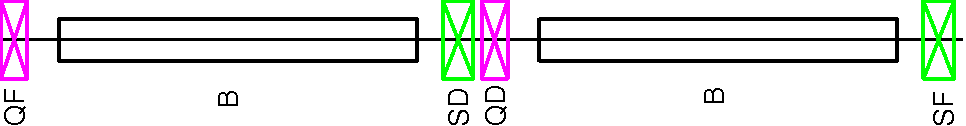
\includegraphics[width=0.95\columnwidth]{figures/fodoaf.pdf}
    \caption{Forward arc FODO cell.} 
    \label{f:fodoaf}
  \end{subfigure}
  \vskip\baselineskip
  \begin{subfigure}[b]{\textwidth}
    \centering
    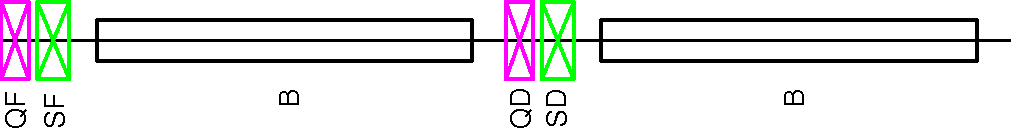
\includegraphics[width=0.95\columnwidth]{figures/fodoar.pdf}
    \caption{Reverse arc FODO cell.} 
    \label{f:fodoar}
  \end{subfigure}
  \caption{
QF, QD: Focusing and defocusing quadrupoles respectively. SF, SD: Sextupoles near focusing and defocusing quadrupoles respectively.
  }
  \label{f:fodofr}
\end{figure}

\begin{figure}[!h]
  \centering
  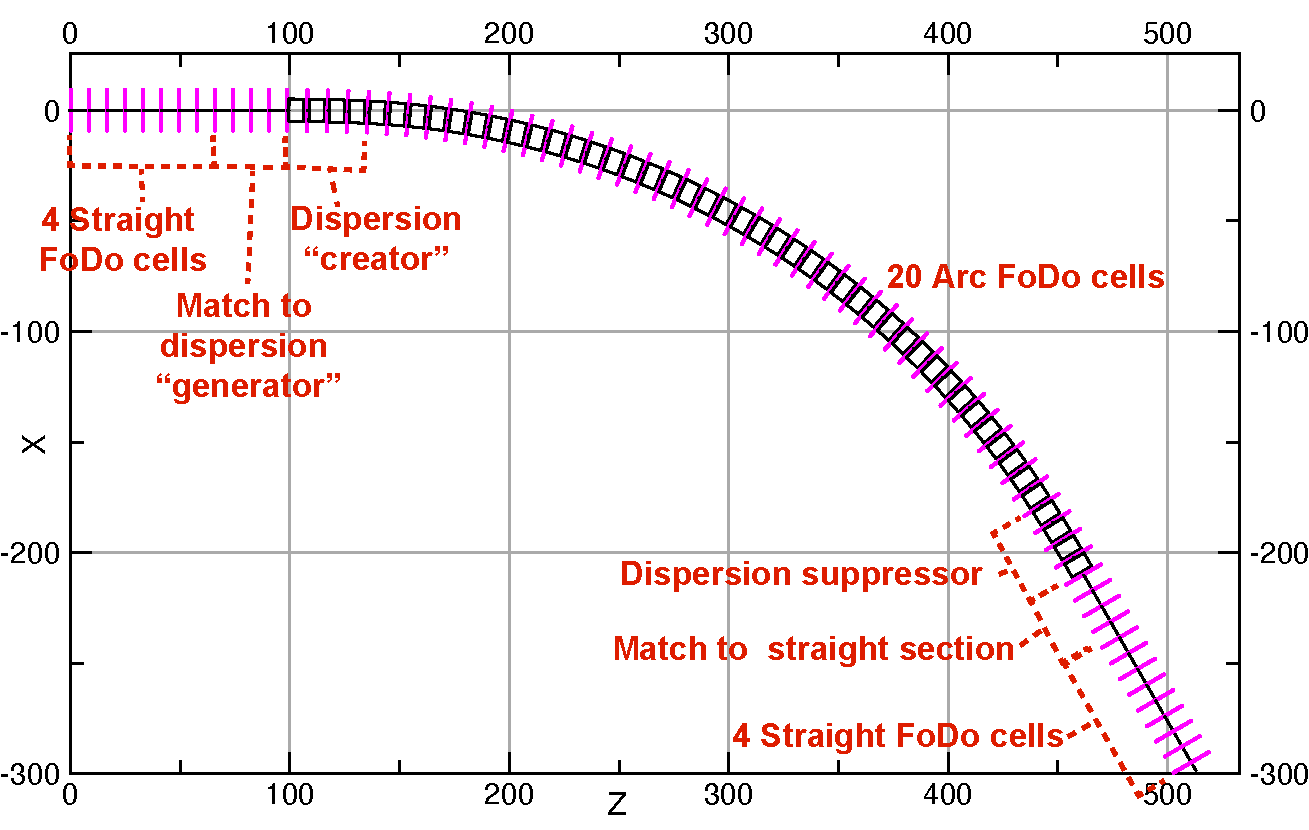
\includegraphics[width=0.8\linewidth]{figures/sextant.pdf}
  \caption{A sextant of the ring.}
  \label{f:sextant0}
\end{figure}

%------------------------------------------------------------------------------
\subsection{Introduction}

In the arc FODO cells of the Electron Storage Ring (ESR), a sextupole, a bend, and a corrector coil all need to fit in between each quadrupole. To accommodate the sextupoles, the quadrupoles cannot be centered between the bends. As a result, there are two types of FODO cells in the ESR: one which has the sextupoles placed before the quadrupoles and one which has the sextupoles placed after the quadrupoles. 
We'll call these the ``forward'' and ``reverse'' cells respectively and are shown in Figs.~\ref{f:fodoaf} and \ref{f:fodoar}. 
This tutorial will use the convention that all FODO cells start with a full-length horizontally-focusing ($K_1 >0$) quadrupole.

The ring is made up 6 sextants as discussed in chapter~\sref{s:ring}.
There are two types of sextants: forward sextants with forward FODO cells and reverse sextants
with reverse FODO cells. The two types of sextants have mirror symmetry with respect to one another.
Each sextant consists of two half-length straight sections with an arc section in between as shown in
Fig.~\ref{f:sextant0}.

The first straight section, in which the dispersion is zero, is followed by a dispersion
``creator'' to match to the periodic dispersion in the arc. After the arc, there is a
dispersion ``suppressor'' to match the dispersion free second straight section. 

%------------------------------------------------------------------------------
\subsection{Example: Forward Arc FODO Cell}

\marginnote{\footnotesize\hspace*{-0.6in}\parbox{1.0in}{
Later in the tutorial the sextupoles and corrector coils will be added in.
}}[0.3in]
%
The phase advance per FODO cell for the lattice to be designed is chosen to be 90$\degree$ to achieve the emittance requirements. Construction of the forward arc FODO cell without sextupoles will be
demonstrated below. Left as an exercise will be the construction of the reverse arc FODO cell without sextupoles along with the forward and reverse straight section FODO cells. Example files can be found in the \vn{/lattices/1_FoDoA/a_Arc/} directory.

\begin{figure}[h!]
  \includegraphics*[width=0.95\columnwidth]{figures/FODOaf-dim.pdf}
  \caption{\label{f:FODOaf}Forward arc FODO cell with lengths specified.}
\end{figure}

\marginnote{\footnotesize\hspace*{-0.6in}\parbox{1.0in}{
See the Bmad manual for details on the different types of elements.
}}[0.15in]
%
Figure \ref{f:FODOaf} shows the lengths of each element in the forward arc FODO cell. The ESR uses rectangular bends (rbends) in the arcs. 
Note: In \bmad, following the MAD convention, the length \vn{L} of an rbend in the lattice file specifies the 
\vn{chord} length, whereas for sector bends (sbends) it specifies the arc length.
See the \vn{Bends: Rbend and Sbend} section in the \bmad manual for more details. 
When \vn{rbend}s are read in, \bmad will convert them to \vn{sbend}s, will set \vn{L_chord}
equal to the input \vn{L}, and will set \vn{L} equal to the true arc length.

Our collider ring with have 132 arc FODO cells, and so each bend must precess the orbit by an angle $2\pi/(2 * 132)$. Choosing initially arbitrary quadrupole strengths \vn{K1}, the \bmad file for this lattice is:
\begin{code}
! Lattice file: fodoAF0.bmad
parameter[p0c]      = 1.7846262612447E10 ! Reference momentum in eV
parameter[particle] = Electron 
parameter[geometry] = closed ! Calculates the periodic Twiss parameters

QF: Quadrupole, L = 0.5, K1 =  0.4
QD: Quadrupole, L = 0.5, K1 = -0.4
B: Rbend, L = 6.86, angle = pi/132
D1: Drift, L = 0.609
D2: Drift, L = 1.241

FODOAF: line = (QF, D1, B, D2, QD, D1, B, D2)
use, FODOAF
\end{code}

Make sure you are in the directory \vn{/lattices/1_FoDoA}.
On the command line, the lattice can be opened in \tao using the command 
\begin{code}
tao -lat fodoAF0.bmad
\end{code} 
where the ``\vn{-lat}'' flag is short for \textbf{-lattice} and the argument following this flag 
needs to be the name of the Bmad lattice file being analyzed. 
Specifying a lattice on the command line will override any default lattice specified in the \vn{tao.init}
file. 
In this case, the \vn{tao.init} file does not specify a lattice so the \vn{-lat} flag is needed on the command line.

When \tao is started, a plot window will open showing the beta functions, dispersion, orbit, and lattice layout. If the plot window is too large for the screen, the \vn{-geom} flag followed by a width and height in the format \vn{<width>x<height>} can be used to adjust the window size. For example:
\begin{code}
tao -lat fodoAF0.bmad -geom 400x400
\end{code}
To view a summary of all the flags, use the command: 
\begin{code}
tao -help
\end{code}
After opening the above lattice in \tao, the \vn{show lattice} command can be used to view the lattice:
\begin{code}
Tao> sho lat     ! Abbreviations are acceptable so "sho lat" works.
# Values shown are for the Exit End of each Element:
# Index  name      key                       s       l    beta   phi_a ...
#                                                            a   [2pi] ...
      0  BEGINNING Beginning_Ele         0.000     ---   43.90   0.000 ... 
      1  QF        Quadrupole            0.500   0.500   43.90   0.002 ...
      2  D1        Drift                 1.109   0.609   38.69   0.004 ...
      3  B         Sbend                 7.969   6.860    3.97   0.098 ...
      4  D2        Drift                 9.210   1.241    2.39   0.164 ...
      5  QD        Quadrupole            9.710   0.500    2.39   0.198 ...
      6  D1        Drift                10.319   0.609    2.98   0.234 ...
      7  B         Sbend                17.179   6.860   33.65   0.354 ...
      8  D2        Drift                18.420   1.241   43.90   0.359 ...
      9  END       Marker               18.420   0.000   43.90   0.359 ...
\end{code}
%
\marginnote{\footnotesize\hspace*{-0.6in}\parbox{1.1in}{
\bmad always includes a BEGINNING element at the beginning.
}}[-1.7in]
%
\marginnote{\footnotesize\hspace*{-0.6in}\parbox{1.0in}{
By default, \bmad puts an END marker element at the end
}}[-0.5in]
%
By default, \tao, will print values evaluated at the downstream \textbf{end} of elements (the end where particles exit the element).
To print information evaluated at the middle or beginning of each element, include the \vn{-middle} or \vn{-beginning} flags in the \vn{show lat} command respectively.

To see the phase advance at the end of the lattice, use the\vn{show element end} command:
%
\marginnote{\footnotesize\hspace*{-0.6in}\parbox{1.0in}{
``show ele 9'' also works.
}}[0.2in]
%
\begin{code}
Tao> show element end
Element # 9
Element Name: END
Key: Marker
S_start, S:     18.420324,     18.420324
Ref_time_start, Ref_time:  6.144359E-08,  6.144359E-08

Attribute values [Only non-zero values shown]:
    1  L                           =  0.0000000E+00 m
                            ...
Twiss at end of element:
                          A              B       ...
  Beta (m)        43.89736699     2.38487039  |   0.00000000   0.00000000  ...
  Alpha           -4.42108656     0.34433533  |   0.00000000   0.00000000  ...
  Gamma (1/m)      0.46804644     0.46902625  |   Gamma_c =   1.00000000   ...
  Phi (rad)        0.00000000     0.00000000            X              Y    
  Eta (m)          0.38412123     0.00000000     0.38412123     0.00000000 ...
  Etap             0.03789803     0.00000000     0.03789803     0.00000000 ...
  dEta/ds          0.03789803     0.00000000     0.03789803     0.00000000 ...
  Sigma            0.00066663     0.00000011     0.00000000     0.00000000

Orbit:  Electron   State: Alive
         Position[mm] Momentum[mrad]        Spin   | ...
  X:       0.00000000     0.00000000               | ...
  Y:       0.00000000     0.00000000               | ...
  Z:       0.00000000     0.00000000               | ...
\end{code} 
%
\marginnote{\footnotesize\hspace*{-0.6in}\parbox{1.0in}{
\vn{Phi} is the betatron phase.
}}[-1.6in]
%
\tao calculates the Twiss parameters of the eigenmodes of the 1-turn matrix. For an uncoupled ring, the \vn{A} mode corresponds to what other programs label the horizontal (x) Twiss, and the \vn{B} mode corresponds to the vertical (y) Twiss.

%------------------------------------------------------------------------------
\subsubsection{Tao.init File}

\marginnote{\footnotesize\hspace*{-0.6in}\parbox{1.0in}{
Additionally, \tao has an interface with Python allowing use of Python based optimizers. 
}}[0.2in]
%
Given our arbitrary choice of quadrupole strengths, the phase advance at the end of our FODO cell is not 90$\degree$. In order to determine what strengths will produce the desired phase advance, the optimizers built into \tao can be used. To perform an optimization, \vn{data} and \vn{variables} must be defined in a \vn{tao.init} file. A \vn{tao.init} file is also useful if you'd like \tao to run with special settings, e.g. a 400x400 plot page size (so the \vn{-geom} flag does not need to be included when running \tao), or even custom plots. In order to determine the correct quadrupoles strengths, for a 90$\degree$ phase advance, the \vn{tao.init} file might look like:

\begin{code}
! tao.init file
&tao_plot_page                    
  plot_page%size = 400, 400    ! Sets the plot page size 
  plot_page%text_height = 8    ! Makes the plot page text size smaller
  plot_page%n_curve_pts = 5000 ! Adds more sampled points to the plots
/

&tao_d2_data                      
  d2_data%name = "phase"
  n_d1_data = 1
/

&tao_d1_data
  ix_d1_data = 1
  datum(1) = "phase.a" "" "" "end" "target" 1.570796326794897 10.0
  datum(2) = "phase.b" "" "" "end" "target" 1.570796326794897 10.0
/

&tao_var
  v1_var%name = "quads"
  var(1:2)%ele_name = "QF", "QD"
  default_step = 1e-6
  default_attribute = "k1"
/
\end{code}

There's a lot going on here, so let's decompose each ``\textbf{namelist}'' in this file.

%------------------------------------------------------------------------------
\subsubsection{Plotting}

The first namelist, \vn{tao_plot_page}, tells \tao to open with a plot window with a size of 400x400, a text height of 8pt, and include 5,000 points for each plot. The last setting will be useful when looking at the betas for the entire ring, as aliasing may be present with the default settings causing plotting artifacts. 

%------------------------------------------------------------------------------
\subsubsection{Optimization Data Setup}

\begin{figure}[h!]
  \centering
  \includegraphics*[width=0.5\columnwidth]{figures/data-tree.pdf}
  \caption{\label{f:datatree} \tao's tree structure for datums.
  A \vn{d2_data} structure holds an array of \vn{d1_data} structures and
a \vn{d1_data} structure holds an array of datums.}
\end{figure}

\vn{Data:} The next two namelists, \vn{tao_d2_data} and \vn{tao_d1_data}, define the \textbf{data} of the optimization. ``\vn{Data}" are the conditions that we wish to satisfy via optimization. 
In this case, wanted is to make the horizontal and vertical phase advances 90$\degree$ from start to end. 
A quick look at the ``\vn{Tao Data Types}" section in the ``\vn{Data}" chapter of the \tao manual shows that 
the desired data types are called \vn{phase.a} and \vn{phase.b}. 

Fig.~\ref{f:datatree} shows how data is organized in a three level tree-structure which
serves as an aid to the user in keeping the data organized. 
At the top level, \vn{d2_data} structures are defined.
A \vn{d2_data} structure is defined with a \vn{tao_d2_data} namelist.
In this case, there is a single \vn{d2_data} structure named ``\vn{phase}''.
Every \vn{d2} structure has an array of \vn{d1_data} structures under it. In this example there is only one
(\vn{n_d1_data} = 1) and this \vn{d1} structure is defined in the \vn{tao_d1_data} namelist below the \vn{tao_d2_data}
namelist. Every \vn{d1_data} structure has an array of \vn{data} structures with each \vn{data} structure representing
a single datum. In this example there are two datums, the first for \vn{phase.a} and the second for \vn{phase.b}.

While this example used a single \vn{d2_data} and a single \vn{d1_data} structure, a differing organization could
have been used and each datum could have been assigned its own separate \vn{d2_data} and a single \vn{d1_data} structures.
Ultimately, the tree organization has no impact on the outcome of the optimization. 

The datums for the optimization are defined on the lines
\begin{code}
datum(1) = "phase.a" "" "" "end" "target" 1.570796326794897 10.0
datum(2) = "phase.b" "" "" "end" "target" 1.570796326794897 10.0
\end{code}
The syntax for setting datums is discussed in the ``Data and Constraint Initialization" section of the ``Initialization" chapter of the \tao manual. 
Basically, the datums will be assigned  ``\vn{model}'' values which are the horizontal and vertical mode phase advances at the \vn{END} element of the FODO cell, and the optimizer will adjust variable settings to try to get these \vn{model} values equal to what is called the ``\vn{measured}'' values which are set to $\pi/2$ as shown above. 

Optimization involves minimization of a merit function  $\cal M$ which is evaluated
using the formula
\begin{equation}
  {\cal M} \equiv 
    \sum_{i} w_i \, \bigl[ \delta D_i \bigr]^2 + 
    \sum_{j} w_j \, \bigl[ \delta V_j \bigr]^2
  \label{m1}
\end{equation}
where the first sum is a sum over the \vn{data} and the second sum is a sum over the \vn{variables}. 
The $w_i$ and $w_j$ are weights specified by the user and the $\delta D_i$ and
$\delta V_j$ are functions of the data and variables. The merit function is discussed in depth in
the ``Optimization" chapter in the \tao manual.

The datums defined above both have weights of 10.0. Datum weights can have a large effect on optimizations. Often times, the best
way to choose the correct weight is trial and error (is the optimization converging well or not?). 

The datums defined above both use a \vn{merit_type} that is set to "\vn{target}". 
In this case, $\delta D$ in \Eq{m1} is evaluated using the equation
\begin{code}[mathescape]
$\delta D$ = model - meas
\end{code}
where \vn{model} is the value as calculated from the lattice and \vn{meas} is the
``\vn{measured}'' value as set on the datum line.
In this case, the \vn{meas} value is $\pi/2$ for both datums.

Datum names are in the form
\begin{code}
<d2-data-name>.<d1-data-name>[datum-index]
\end{code}
In this case, the \vn{d2_data} structure has the name (set by \vn{d2_data%name} in the file) of "\vn{phase}".
The name of the \vn{d1_data} structure is not specified in the file and so gets the default name of ``\vn{1}"
(if there were other \vn{d1_data} structs associated with this \vn{d2_data} structure, the default names
would be ``\vn{2}", ``\vn{3}", etc.). The datums have names
\begin{code}
phase.a datum: phase.1[1]     ! Can be shortened to phase[1]
phase.b datum: phase.1[2]     ! Can be shortened to phase[2]
\end{code}
Since there is only one \vn{d1_datum} here the ``\vn{.1}'' specifier can be omitted. The \vn{show data}
command will display a list of defined \vn{d2_data}:
\begin{code}
Tao> show data
  Name                                 Using for Optimization
  phase[1:2]                                     Using: 1:2
\end{code}

To see information on a particular \vn{d2_data} structure, use the command \vn{show data <d2>} where \vn{<d2>}
is the name of the structure. In this case:
\begin{code}
Tao> show data phase
Data name: phase.1
                                                                   |   Useit
                     ... Ele        Meas        Model       Design | Opt  Plot
 1  phase.a <target> ... END  1.57079E+0   2.25845E+0   2.25845E+0     T     F
 2  phase.b <target> ... END  1.57079E+0   2.260399+0   2.26039E+0     T     F
\end{code}
The \vn{design} value is the value of the ``\vn{design}" lattice which is a lattice \tao creates representing the
lattice that was read in (discussed in depth in chapter~\sref{s:three.lat}). 
The parameters in the design lattice are fixed and cannot change. 
This is in contrast to the ``\vn{model}" lattice where the parameters are changeable and it is the quadrupole
strengths of the model lattice which will be varied in the optimization. 
In this case, the merit function is calculated using the difference \vn{model - meas} (see above), the design lattice does not influence the present optimization.

To see information on a particular datum, use the \vn{show data <datum>} where \vn{<datum>} is the name
of the datum. For example:
\begin{code}
Tao> show data phase[1]

%ele_name          = "END"
... etc...
%data_type         = "phase.a"
... etc...
%model             =   2.25845820E+00
%design            =   2.25845820E+00
... etc...
%weight            =   1.00000000E+01
%exists            = T
%good_model        = T
%good_design       = T
%good_base         = T
%good_meas         = T
... etc...
%useit_plot        = F
%useit_opt         = T
\end{code}
The \vn{useit_opt} logical indicates whether the datum will be used when the merit function is
evaluated. For example, if the \vn{meas} value has not been set, \tao will set \vn{good_meas} to
False and this will cause \tao to set \vn{useit_opt} to False.

%------------------------------------------------------------------------------
\subsubsection{Optimization Variable Setup}

The last namelist, \vn{tao_var}, in the above \vn{tao.init} file defines the \textbf{variables} of the optimization
\begin{code}
&tao_var
  v1_var%name = "quads"
  var(1:2)%ele_name = "QF", "QD"
  default_step = 1e-6
  default_attribute = "k1"
/
\end{code}
\textbf{variables are the things to vary in the optimization to satisfy the conditions defined by the data}. Variables are grouped
in a tree structure just like data except for variables there are only two layers instead of the three for data.
The top layer is a set of \vn{v1_var} structures. In this case there is a single \vn{v1_var} structure called
"\vn{quads}". Every \vn{v1_var} structure has an array of \vn{variables}. In this case, the \vn{quads} \vn{v1_var} structure has a two variable array with the variables controlling the \vn{k1} attribute of the \vn{QF}, and \vn{QD} quadrupoles respectively. 
To calculate derivatives for the optimization, \tao uses finite differences and so a step size must be specified.
The step size can be different for different variables but here a default value of \vn{1e-6} is used that will
be applied to all the variables. 
Variables can have weights which affects the merit function.
Weights for variables are useful when there are ``degeneracies" or near-degeneracies where, without variable weights, the optimizer can find solutions with small merit function values with variables having unphysically large values. The weights can
constrain variables to have reasonable values. In this case there are no degeneracies and variable weights are not needed.

To refer to an individual variable use the syntax:
\begin{code}
v1-var-name[var-index]
\end{code}
where \vn{var-index} is the index of the variable. For example, the first variable in the \vn{quad}
structure is \vn{quad[1]}, etc.

When running \tao, the \vn{show variable} command can be used to view a list of the \vn{v1_vars} defined
\begin{code}
Tao> show var
       Name                                      Using for Optimization
    quads[1:2]                                   1:2
\end{code}
The \vn{show variable <v1>} can be used to show information on a particular \vn{v1_var} named \vn{<v1>}
\begin{code}
Tao> show var quads
  Variable      Slave Parameters   Meas         Model        Design  Useit_opt
  quads[1]      QF[K1]         0.0000E+00    4.0000E-01    4.0000E-01       T
  quads[2]      QD[K1]         0.0000E+00   -4.0000E-01   -4.0000E-01       T
\end{code}
And the \vn{show variable <var>} can be used to show information on a particular variable named \vn{<var>}
\begin{code}
Tao> show var quads[2]
%ele_name         = "QD"
%attrib_name      = "K1"
... etc...
%model            =  -4.00000000E-01
... etc...
%exists           = T
%good_var         = T
%good_user        = T
%good_opt         = T
%useit_opt        = T
\end{code}

%------------------------------------------------------------------------------
\subsubsection{Running an Optimization}

To see what data and what variables are being used in the optimization, use the \vn{show data} and
\vn{show variables} commands as discussed above. To see optimizer parameters, use the \vn{show optimizer} command:
\begin{code}
Tao> show opti
Data Used:
  phase[1:2]                                     Using: 1:2
Variables Used:
  quads[1:2]                                     Using: 1:2

optimizer:        "lm"
Global optimization parameters (use "set global" to change):
  %de_lm_step_ratio              =   1.00000000E+00
  %de_var_to_population_factor   =   5.00000000E+00
  %lm_opt_deriv_reinit           =  -1.00000000E+00
  ...
\end{code}
There are many parameters associated with optimization and it is important to carefully consider
what values these parameters have in order to be able to have a successful optimization.

To see how the merit function is being evaluated, use the \vn{show constraints} command:
\begin{code}
Tao> show cons

Constraints                 ...  Ele/S    Meas-or-Lim    Model       Merit      
phase[1]   phase.a <target> ...  END      1.5708E+00   2.2585E+00  4.729E+00
phase[2]   phase.b <target> ...  END      1.5708E+00   2.2604E+00  4.756E+00
quads[1]   QF[K1]           ...  0.50    -1.0000E+30   4.0000E-01  0.000E+00
quads[2]   QD[K1]           ...  9.71    -1.0000E+30  -4.0000E-01  0.000E+00    

 figure of merit: 9.484309E+00

! Top 10
Constraints                 ...  Ele/S    Meas-or-Lim    Model       Merit     
phase[2]   phase.b <target> ...  END      1.5708E+00   2.2604E+00  4.756E+00
phase[1]   phase.a <target> ...  END      1.5708E+00   2.2585E+00  4.729E+00
quads[2]   QD[K1]           ...  9.71    -1.0000E+30  -4.0000E-01  0.000E+00
quads[1]   QF[K1]           ...  0.50    -1.0000E+30   4.0000E-01  0.000E+00 
\end{code}
This shows, among other things, that the value of the merit function is 9.48 and that the largest
contributor to the merit function by a hair is \vn{phase[2]} which has a contribution of 4.756 which is about
50\% of the total merit function.
In this optimization, the variables do not contribute to the merit function.

There are several optimizers that can be used as detailed in the \tao manual. For global optimization use
the \vn{de} (Differential Evolution) optimizer. All other optimizers will only converge to the local optimum
but will converge faster than \vn{de}.
In this case, the optimum is local so the lm (Levenburg-Marquardt) optimizer will be used which is the default:
\begin{code}
Tao> run
Optimizing with: lm
Type ``.'' to stop the optimizer before it's finished.
[INFO] tao_dmodel_dvar_calc:
    Remaking dModel_dVar derivative matrix.
    This may take a while...

  Cycle      Merit    A_lambda
    1    4.3831E-01   1.00E-04
    2    5.7875E-02   1.00E-05
    3    8.5664E-03   1.00E-06
    ... etc...
   20    1.7768E-16   1.00E-23
Written: var1.out
   21    1.7768E-16   0.00E+00
\end{code}
The Merit value is now about $10^{-16}$ showing good convergence which can be seen by examining the data:
\begin{code}
Tao> show data phase
Data name: phase.1
                                                                     |  Useit
                     ... Ele        Meas         Model        Design | Opt Plot
 1  phase.a <target> ... END  1.570796E+0   1.570796E+0   2.258458E+0    T    F
 2  phase.b <target> ... END  1.570796E+0   1.570796E+0   2.260399E+0    T    F
\end{code}
And the model lattice has the correct phase advance.

Use \vn{write bmad fodoAF.bmad} after optimizing to create a new lattice file with name \vn{fodoAF.bmad} having the optimized quadrupole strengths. 
Note that \vn{fodoAF.bmad} will contain the beginning periodic Twiss, dispersion, and
orbit (only non-zero values are put in the file so the orbit does not explicitly appear in this instance). This is very useful if the
\vn{geometry} is switched from \vn{closed} to \vn{open} as will be discussed in the following chapter.

%----------------------------------------------------------
\subsection{Exercises}
\label{s:fodo.ex}

\begin{enumerate}[leftmargin=*]
\item {\bf Reverse arc FODO:} Construct the reverse arc FODO cell without sextupoles, and determine the quadrupole strengths for a 90$\degree$ phase advance. Let the optimized lattice file name be \vn{fodoAR.bmad}.
%
\item {\bf Forward straight section FODO:} Replace the dipoles in the forward cell by a drift (empty space) of length 5.855m and name the drifts \vn{DB}. This length is chosen to produce the same straight section length as in the RHIC tunnel. Additionally, rename the horizontally-focusing and defocusing quadrupoles \vn{QFSS} and \vn{QDSS} respectively. Which quadrupole strengths lead to 90 degrees phase advance in both planes? 
Use the name \vn{fodoSSF.bmad} for the optimized lattice file. Note: files are in \vn{1_FODO/b_SS/F}
%
\item {\bf Reverse straight section FODO:}  Replace the dipoles in the reverse cell by a drift of length 5.855m and name the drifts \vn{DB}. Rename the horizontally-focusing and defocusing quadrupoles \vn{QFSS} and \vn{QDSS} respectively. Which quadrupole strengths lead to 90 degrees phase advance in both planes? 
Use the name \vn{fodoSSR.bmad} for the optimized lattice file. 
These quadrupole strengths should be exactly the same as in \vn{fodoSSF.bmad}
%
\item {\bf Analytical FODO cell:} Using a FODO model with the same total length as constructed above but
with zero length quadrupoles, and no bends. Calculate by hand the appropriate quad strengths that lead to a 90 degrees phase advance in x and y. What are the beta functions at the thin quads? How do the quad strengths and beta functions compare to above?
%
\item {\bf Forward and Reversed Cells:} Check that your forward and reverse arc FODO cells that both start with focusing quads have different periodic beta and alpha functions. Check also that both cells, for the same phase advance of 90 degrees have exactly the same quadrupole strength. Explain why this is so
%
\item {\bf L, L_arc, and L_chord:} For \vn{rbend} elements, to be consistent with the MAD program, 
the input ``\vn{l}" length in the lattice file is used as the chord length. On input, the \vn{rbends} 
are converted to \vn{sbends} and after the conversion \vn{l} will be set to
the true arc length. For the \vn{rbends} in the above lattice, what is the
difference of the values between these two lengths? 
[Hint: Use the ``show ele" command.]
%
\item {\bf show lattice command:} The \vn{show lattice} command is very powerful (and has a lot of options). 
Can you figure out what the following command shows?
\begin{code}
Tao> show lat -attrib k1 quadrupole::*
\end{code}
%
\item {\bf show data <datum> command:} An individual datum is a complicated beast and the output of the \vn{show data <datum>} command reflects this. Look at the full (not abridged output above) output and by reading the
\tao manual see if you can make sense of the individual components.
%
\item {\bf The \vn{good_user} logical:} One component of a datum or variable is \vn{good_user} which is set by
the user and controls whether the datum or variable will be used in the optimization. Commands to control \vn{good_user}
are \vn{use}, \vn{veto} and \vn{restore}. Play around with these commands to see how changing this affects
the optimization.
\end{enumerate}

\newpage

%------------------------------------------------------------------------------
%------------------------------------------------------------------------------
\section{Dispersion Suppressor}
\label{s:dispersion}

%------------------------------------------------------------------------------
\subsection{Introduction}
To connect an arc to the following straight section in a sextant, the dispersion 
in the straight section must be suppressed to zero while minimally changing the betas. 
For a 90$\degree$ lattice, this can be approximately achieved by using two equivalent arc FODO cells with the bends at half-strength.
To get the dispersion and dispersion derivative at the end of the dispersion suppressor exactly
zero, the last two quadrupoles can be minimally varied.

\begin{figure}[!h]
  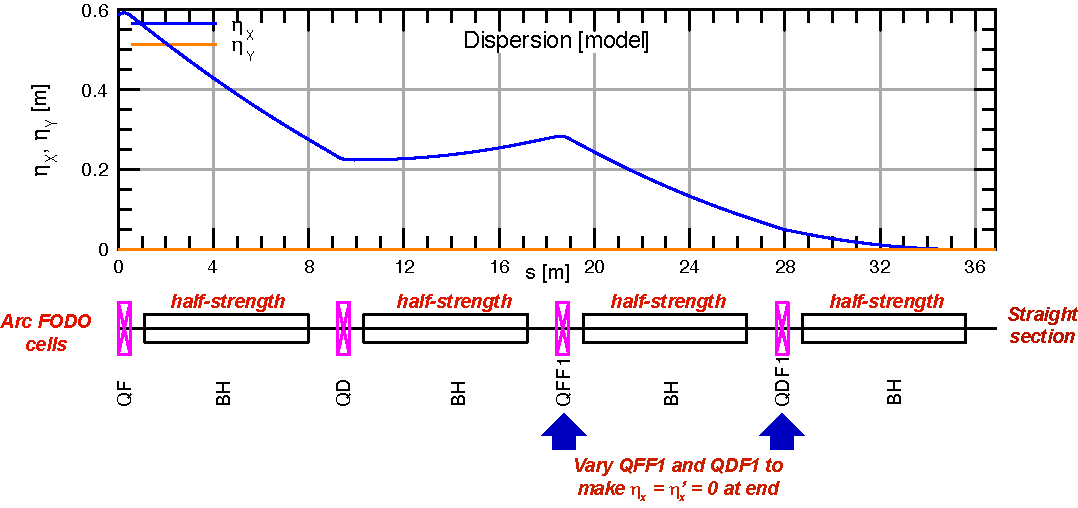
\includegraphics[width=0.95\columnwidth]{figures/dispsup.pdf}
    \caption{Dispersion suppressor.}
    \label{f:dispsup}
\end{figure}

%------------------------------------------------------------------------------
\subsection{Example: Forward Dispersion Suppressor Creation}

The procedure for creating the forward dispersion suppressor is outlined below. 
The reverse dispersion suppressor construction is left as an exercise. 
The example files can be found in the \vn{/lattices/2_DispSuppress/F/} directory.

To create the forward dispersion suppressor:
\begin{enumerate}[leftmargin=*]
\item Create a copy of the \vn{fodoAF.bmad} file, which contains the optimized quadrupole strengths for the 90$\degree$ phase advance FODO cell.
%
\item In this new copy, set \vn{parameter[geometry]} equal to \vn{open}. This tells \bmad to \textit{not} calculate the periodic betas, instead propagating the initial betas specified in the lattice file (which in this case, are the beginning periodic betas in the arc cells) through the lattice.

\begin{code}
parameter[geometry] = open     ! (2): Set geometry to open  
\end{code}
%
\item Define a new half-strength bend element and the two special quadrupoles to vary to make $\eta_x=\eta_x'=0$. The strengths will be calculated via optimization. Because these special quadrupoles are in the forward sextant (F), and are the first ``special'' quadrupoles (1), use the names \vn{QFF1} and \vn{QDF1} (that is, add an \vn{F1} suffix to the original quadrupole names).
%
\begin{code}
! (3): Define half bend and quads for dispersion suppression 
BH: rbend, L = 6.86, angle=pi/132/2
QFF1: Quadrupole, L = 0.5, K1 = 0.3
QDF1: Quadrupole, L = 0.5, K1 = -0.3
\end{code}
%
\item Define and use the new line as in Fig.~\ref{f:dispsup} containing the half bends and special quads. Since this is the forward dispersion suppressor, use the name \vn{DISPSUPF} for the line. 
\begin{code} 
! (4): Define the new line for half bends
DISPSUPF: line = (QF, D1, BH, D2, QD, D1, BH, D2,
                  QFF1, D1, BH, D2, QDF1, D1, BH, D2)
use, DISPSUPF
\end{code}
The completed initial lattice file containing these changes is provided in the example file named \vn{dispsupF0.bmad}. 
%
\item
A \vn{tao.init} file is needed to define the optimization parameters. This might look like:
\marginnote{\footnotesize\hspace*{-0.6in}\parbox{0.8in}{
Use the "show opt" to see opt params.
}}[1.9in]
%
\begin{code}
&tao_plot_page
  plot_page%size = 400, 400
  plot_page%text_height = 8
  plot_page%n_curve_pts = 5000
/

! Set the number of cycles to 1000 to avoid having to type "run" less
&tao_params
  global%n_opti_cycles = 100
  global%n_opti_loops = 100
/

&tao_d2_data
    d2_data%name = "disp"
    n_d1_data = 1
/

&tao_d1_data
  ix_d1_data = 1
  datum(1) = "eta.x" "" "" "end" "target" 0 10
  datum(2) = "deta_ds.x" "" "" "end" "target" 0 10
/

&tao_var
  v1_var%name = "quads"
  var(1:2)%ele_name = "QFF1", "QDF1"
  default_step = 1e-6
  default_attribute = "k1"
/
\end{code}

This \vn{tao.init} file has a namelist \vn{tao_params} in which \vn{n_opti_cycles}, the number of optimization cycles, is set equal to 100 (the default is 20). 
When the optimizer goes through \vn{n_opti_cycles}, this
is called a \vn{loop}. Before each loop, the derivatives of how much the \vn{data} changes with change in
\vn{variable} is computed. Periodic recomputation is needed since lattices are never linear and so the derivatives change as variables are varied. Also in the \vn{tao_params} namelist the number of loops,
which is set by \vn{n_opti_loops}, is set to 100 (the default is one).
These are two of many parameters that can be set to customize the \tao experience. See the \tao manual for more options.

The \vn{tao.init} file has two datums, one for the horizontal dispersion \vn{eta.x} and one for its slope \vn{deta_ds.x}. 
Both are desired to be exactly zero at the end of the lattice and they have equal weight. 
Additionally, the variables are the k1 strength of the two special quadrupoles \vn{QFF1} and \vn{QDF1}. 
%
\item
Starting \tao with the new \vn{tao.init} file, the \vn{show constraints} command can be used to
verify that the optimization is set up correctly:
\begin{code}
Tao> show cons

Constraints                  ...   Ele/S  Meas-or-Lim    Model       Merit 
disp[1]   eta.x <target>     ...   END      0.0000E+00   5.1814E-02  2.685E-02
disp[2]   deta_ds.x <target> ...   END      0.0000E+00   3.9512E-03  1.561E-04
quads[1]  QFF1[K1]           ...   18.92   -1.0000E+30   3.0000E-01  0.000E+00
quads[2]  QDF1[K1]           ...   28.13   -1.0000E+30  -3.0000E-01  0.000E+00
Constraints                  ...   Ele/S  Meas-or-Lim    Model       Merit 

 figure of merit: 2.700305E-02

! Top 10

Constraints                  ...   Ele/S   Meas-or-Lim    Model       Merit
disp[1]   eta.x <target>     ...   END       0.0000E+00   5.1814E-02  2.685E-02
disp[2]   deta_ds.x <target> ...   END       0.0000E+00   3.9512E-03  1.561E-04
quads[2]  QDF1[K1]           ...   28.13    -1.0000E+30  -3.0000E-01  0.000E+00
quads[1]  QFF1[K1]           ...   18.92    -1.0000E+30   3.0000E-01  0.000E+00
Constraints                  ...   Ele/S   Meas-or-Lim    Model       Merit 

 figure of merit: 2.700305E-02

\end{code}
%
\item
The optimizer can now be run:
\begin{code}
Tao> run
Optimizing with: lm
Type ``.'' to stop the optimizer before it's finished.
[INFO] tao_dmodel_dvar_calc:
    Remaking dModel_dVar derivative matrix.
    This may take a while...

  Cycle      Merit    A_lambda
    1    7.0232E-05   1.00E-04
    2    4.0222E-05   1.00E-05
    3    1.2014E-05   1.00E-06
    ... etc...
  156    1.9259E-33   1.36E+10
Optimizer at minimum or derivatives need to be recalculated.
Written: var1.out
  157    1.9259E-33   0.00E+00
\end{code}
%
\item
The \vn{show data} and \vn{show var} commands can be used to inspect the data and variables:
\begin{code}
Tao> show data disp
Data name: disp.1
                                                                   |   Useit
                      ... Ele       Meas        Model       Design | Opt  Plot
1  eta.x <target>     ... END  0.0000E+00   1.3877E-17   5.1814E-02    T     F
2  deta_ds.x <target> ... END  0.0000E+00   0.0000E+00   3.9511E-03    T     F

Tao> show var quads
Variable   Slave Parameters   Meas         Model        Design   Useit_opt
quads[1]   QFF1[K1]       0.0000E+00    3.1279E-01    3.0000E-01         T
quads[2]   QDF1[K1]       0.0000E+00   -3.1244E-01   -3.0000E-01         T
\end{code}
The dispersion and its slope are 0 or negligibly small so the optimization has been sucessful.
%
\item
Use \vn{write bmad dispsupF.bmad} to create a new lattice file named \vn{dispsupF.bmad} with the optimized quadrupole strengths. This will be the dispersion suppressor for the forward sextants.
\end{enumerate}
%-----------------------------------------------------------------------
\subsection{Exercises}

\begin{enumerate}[leftmargin=*]
\item {\bf Reverse dispersion suppressor:} Construct the reverse dispersion suppressor, optimizing the last two quadrupole strengths for $\eta_x=\eta_x'=0$ exactly at the end for a 90$\degree$ phase advance. How do the two quadrupole values for the reverse dispersion suppressor compare to those obtained in class for the forward suppressor? Name the optimized lattice file name \vn{dispsupR.bmad}.
%
\item {\bf Forward and Reversed Cells:} Check that your forward and reverse cells that both start with focusing quads have different periodic beta and alpha functions. Check also that both cell, for the same phase advance of 90 degrees have exactly the same quadrupole strength. Explain how this can be the correct solution.
%
\item {\bf Dispersion derivative:} \tao calculates a ``dispersion derivative" and a ``momentum dispersion"
which for the $x$ plane are \vn{deta_ds.x} and \vn{etap.x} respectively. What is the difference between the
two? Show that with the lattice being designed they are the same. Hint: See the \bmad manual.
%
\item {\bf Normal mode dispersion:} What is the difference between the horizontal $\eta_x$ and vertical
$\eta_y$ dispersions and the normal mode dispersions $\eta_a$ and $\eta_b$ in the lattice being constructed? 
Verify your answer by checking the
difference for one lattice element (Use the ``show ele" command).
%
\item{\bf Setting optimization parameters:} The \vn{tao.init} file for this chapter sets 
the global parameter 
\vn{global%n_opti_cycles} to 100 and this setting happens when Tao is started.
Besides being able to set this parameter in the initialization file, 
this, and all other parameters, may be set from Tao's
command line. What is the command to set \vn{global%n_opti_cycles}
from the command line?
%
\item {\bf Strength of bends:} [Warning! This is a difficult problem!] 
To a good approximation, a dispersion suppressor between from an arc FODO line to a straight FODO line (where the
straight FODO cells have the same layout as the arc FODO cells except that the bends are replaced by drifts) can be
constructed using two arc FODO cells with the first cell having the bend strengths reduced by a factor $\alpha$
and the second cell with the bend strengths reduced by a factor $1 - \alpha$. In the case of $90^\circ$ FODO
cells, $\alpha$ is 0.5. Note: The approximation is only valid in the case of weak bends. Problem: Prove that this is the case and show that for $60^\circ$ FODO cells the
value of $\alpha$ is zero. 
\end{enumerate}
\newpage

%------------------------------------------------------------------------------
%------------------------------------------------------------------------------
\section{Dispersion Suppressor to Straight Section Twiss Parameter Matching}

%------------------------------------------------------------------------------
\subsection{Introduction}

The periodic betas in the arcs are different from the periodic betas in the straight sections. After suppressing the dispersion to zero, four quadrupoles after the dispersion suppressor are needed to match $\alpha_a$, $\alpha_b$, $\beta_a$, and $\beta_b$ to the periodic betas in the following straight section.
\begin{figure}[!h]
    \centering
    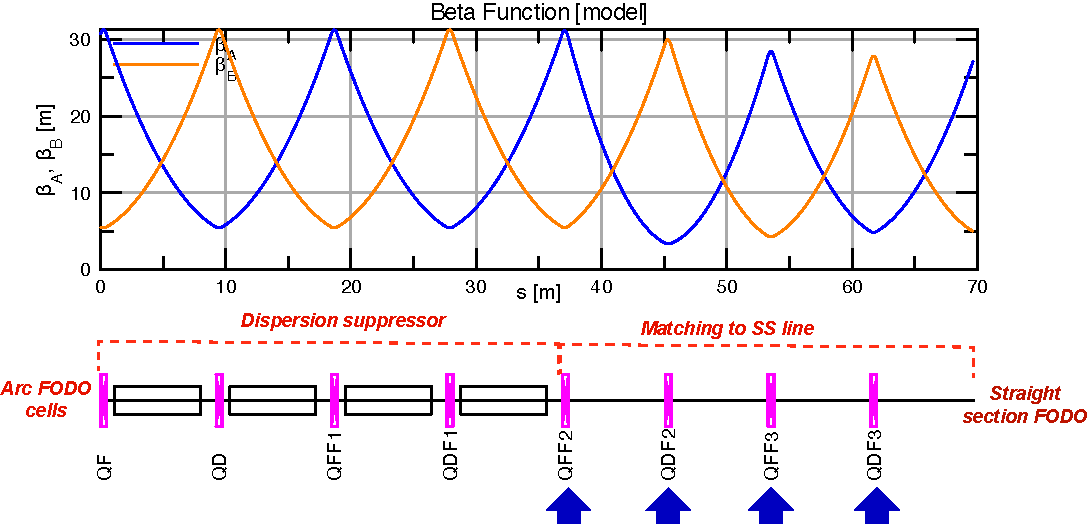
\includegraphics[width=1\linewidth]{figures/match.pdf}
    \caption{Dispersion suppressor match section.}
    \label{f:match}
\end{figure}

%------------------------------------------------------------------------------
\subsection{Example: Forward Matching Section Creation}

The procedure for creating the forward matching section is shown below.
Matching the reverse matching section is left as an exercise. 
The example files can be found in the \vn{/lattices/3_MatchToSS/F/} directory.

To create the forward matching section:
\begin{enumerate}[leftmargin=*]
%
\item Create a copy of the \vn{dispsupF.bmad} file, which contains the optimized dispersion suppressor.
%
\item In this new copy, add the straight section drift \vn{DB}, which was defined previously in Exercises 2 and 3 of section~\ref{s:fodo.ex}.
\begin{code}
! (2): Add straight section (SS) drift DB
DB: Drift, L = 5.855
\end{code}    
%
\item Define four quads for matching to the straight section. Because this is the forward matching section (F), and these are the 2nd and 3rd special QF and QDs, use the names \vn{QFF2}, \vn{QDF2}, \vn{QFF3}, and \vn{QDF3}.
%
\begin{code}
! (3): Define quads for matching to SS (two per plane, 
!      use SS strengths as starting point)
QFF2: Quadrupole, L = 0.5, K1 = 0.351957452649287
QDF2: Quadrupole, L = 0.5, K1 = -0.351957452649287
QFF3: Quadrupole, L = 0.5, K1 = 0.351957452649287
QDF3: Quadrupole, L = 0.5, K1 = -0.351957452649287
\end{code}
%
\item Define the matching to the straight section (SS) line in Fig.~\ref{f:match} containing the matching quads. Because this is the forward matching to SS, Use the name \vn{MSSF}. 
\begin{code} 
! (4): Define the matching to SS line (MSSF)
MSSF: line = ( QFF2, D1, DB, D2, QDF2, D1, DB, D2,  
               QFF3, D1, DB, D2, QDF3, D1, DB, D2)
\end{code}
%
\item 
\marginnote{\footnotesize\hspace*{-0.5in}\parbox{0.8in}{
``F'' stands for Forward.
}}[0.05in]
%
Use the name \vn{ARC_TO_SSF} as the line containing
the combined dispersion suppression and matching to SS line:
\begin{code}
! (5): Define the dispersion suppression and
!       matching to SS line (ARC_TO_SSF)
ARC_TO_SSF: line = (DISPSUPF, MSSF)

use, ARC_TO_SSF
\end{code}
The completed initial lattice file containing these changes is provided in the example files, named \vn{mSSF0.bmad}. 
%
\item
The last four quads need to be optimized so that at the end of the \vn{ARC_TO_SSF} line the betas are equal to the periodic betas in the straight section FODO cells. 
Four datums, one for each of $\alpha_a$, $\alpha_b$, $\beta_a$, and $\beta_b$ at the end of the line, 
need to be defined in the \vn{tao.init} file.  
The ``measure'' (target) values of these datums can be found from the solution lattice \vn{fodoSSF.bmad} obtained in Exercise 2 of Section~\ref{s:fodo.ex}. The variables will be the quadrupole strengths of \vn{QFF2}, \vn{QDF2}, \vn{QFF3}, and \vn{QDF3}. The completed \vn{tao.init} file is provided in the example files.
%
\item
Run the optimizer in \tao a couple times until the merit is extremely small. The merit will be of order $10^{-28}$. The data should look like:
\begin{code}
Tao> show data betas
Data name: betas.1
                                                                    |  Useit
                    ... Ele          Meas        Model       Design | Opt Plot
1  beta.a <target>  ... END   2.7205E+01   2.7205E+01   3.0610E+01     T    F
2  alpha.a <target> ... END  -2.4024E+00  -2.4024E+00  -2.4011E+00     T    F
3  beta.b <target>  ... END   4.9609E+00   4.9609E+00   5.5667E+00     T    F
4  alpha.b <target> ... END   4.8460E-01   4.8460E-01   4.7804E-01     T    F

\end{code}

You can also verify the Twiss parameters are indeed what you need them to be at the \vn{END} element using command \vn{show element END}.
\begin{code}
Tao> show ele END
Element # 33
Element Name: END
......
Twiss at end of element:
                          A              B  
  Beta (m)        27.20598820     4.96091411  ...
  Alpha           -2.40249037     0.48460556  ...
  Gamma (1/m)      0.24891432     0.24891432  ...
......
\end{code}
%
\item
Save the optimized quadrupoles strength by writing a new lattice file \vn{mSSF.bmad}. This will be the matching section in the forward sextants.
\end{enumerate}

%------------------------------------------------------------------------------
\subsection{Exercises}

\begin{enumerate}[leftmargin=*]
\item {\bf Reversed matching section:} Construct the reverse matching section, following the same steps as shown in the example but for the reverse cells. How do your quad values compare to those obtained in class for the forward matching cells? Let the optimized lattice file name be \vn{mSSR.bmad}.
%
\item {\bf Merit Weight:} 
Optimization success or failure can depend heavily on the relative weights used for the data and the variables.
As an example of this, start again with the unoptimized lattice and this time set the weight for the datum 
\vn{beta[1]} to 1E10. This can be done in the lattice file or on the Tao command line with:
\begin{code}
set data betas[1]|weight = 1e10
\end{code}
With this, how well does the optimization do?
\end{enumerate}

\newpage

%------------------------------------------------------------------------------
%------------------------------------------------------------------------------
\section{Machine Coordinates}
\label{s:coords}

\begin{figure}[tb]
  \centering
  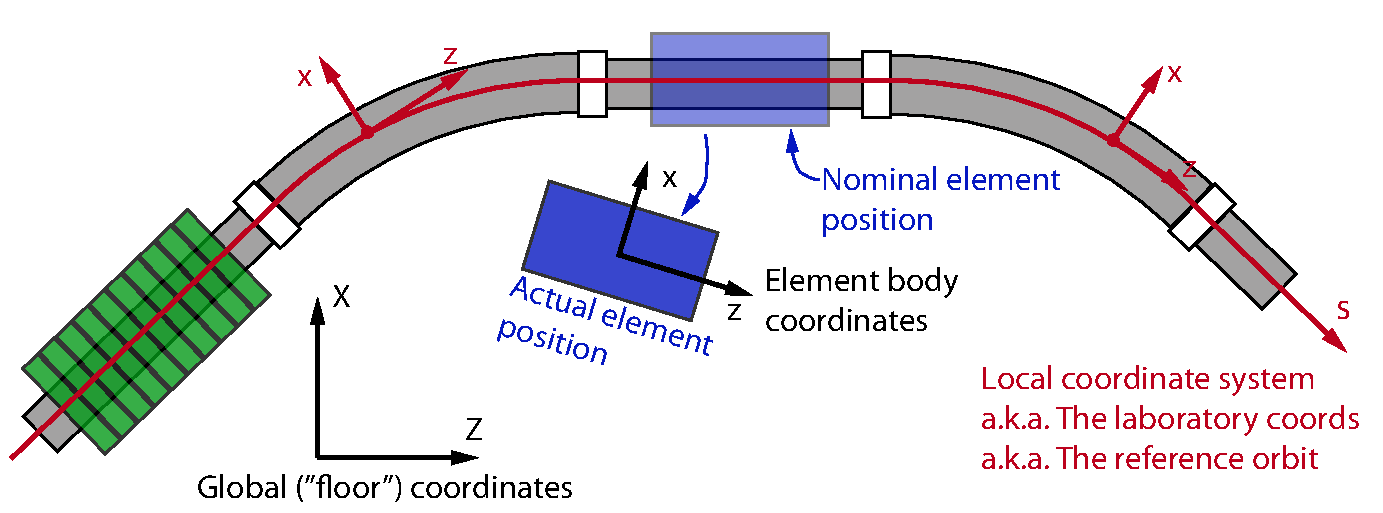
\includegraphics[width=0.9\textwidth]{figures/coordinates.pdf}
  \caption{The three coordinate systems used to describe lattice element positioning:
\vn{Global}, \vn{reference}, and \vn{element body} coordinates.}
  \label{f:coordinates}
\end{figure}

%----------------------------------------------------------
\subsection{Coordinate Systems}
\label{s:coord.sys}

As explained in the \vn{Coordinates} chapter of the \bmad manual, bmad uses three coordinate
systems to describe the positioning of lattice elements as shown in Figure~\ref{f:coordinates}:
\begin{description}
\item[Global Coordinates] \Newline
The \vn{(X, Y, Z)} \vn{global} (also called \vn{floor}) coordinate system (notice that capital
letters are used for the coordinate axes) is independent of the accelerator machine and is "attached" to the building the
accelerator is in. Typically, the \vn{Y}-axis is taken to be pointing vertically up and \vn{(X, Z)}
defines the horizontal plane.
%
\item[Local Coordinates] \Newline
The \vn{global} coordinate system is not convenient for describing where particles are as they move
through the lattice. For this, shown in red, there is the \vn{local} (also called \vn{laboratory},
also called \vn{reference}) curvilinear coordinate system. Laboratory coordinates are also used to
describe the nominal (that is, without any ``misalignments'') position of the lattice elements. The
laboratory coordinates start with a curved line often called the ``\vn{reference trajectory}''. The
distance along the reference trajectory is denoted by $s$. At each point along the reference
trajectory, there is a Cartesian \vn{(x, y, z)} coordinate system with the origin at the reference
trajectory point. The $z$-axis is always tangent to, and the $x$ and
$y$-axes always transverse to the reference trajectory.
%
\item[Element Body Coordinates] \Newline
Elements can be shifted ("misaligned") from their nominal position. To describe things like electric
and magnetic fields or apertures (which can depend upon an element's actual position), \vn{element body}
coordinates are used.  The \vn{element body} coordinates are the coordinates attached to the
physical element. Without any "misalignments", the \vn{element} coordinates correspond to the
\vn{laboratory} coordinates.
\end{description}

\begin{figure}[tb]
  \centering
  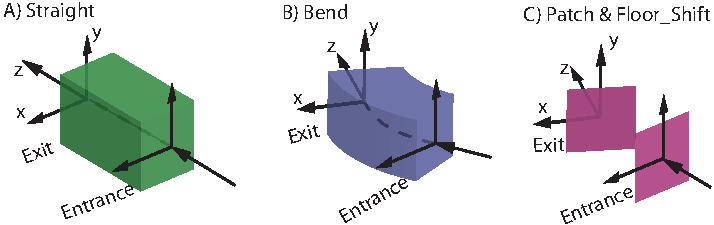
\includegraphics[width=0.9\textwidth]{figures/element-coord-frame.pdf}
  \caption{Lattice element geometry types: \vn{Straight}, \vn{bend}, and \vn{patch}. All elements have an 
\vn{entrance} coordinate system and an \vn{exit} coordinate system.}
  \label{f:body.types}
\end{figure}

%----------------------------------------------------------
\subsection{Element Geometry Types}

All lattice elements have an ``\vn{entrance}'' end and an ``\vn{exit}'' end. Normally a particle
will enter the element at the \vn{entrance} end and exit at the \vn{exit} end but it is possible to
simulate particles going backwards or have lattice elements that are reversed longitudinally.

Lattice elements in \bmad have one of four geometry types. Three of them will be discussed here and
are shown in Figure~\ref{f:body.types}. [The fourth geometry type, used for X-ray simulations, is
used with \vn{mirror}, \vn{multilayer_mirror}, and \vn{crystal} elements.] These three types are
called \vn{straight}, \vn{bend} and \vn{patch} based upon how the $(x, y, z)$ laboratory coordinates
transform as a function of the longitudinal \vn{s} position from the \vn{entrance} end of the
element to the \vn{exit} end.
\begin{description}
\item[Straight Geometry] \Newline
The straight geometry, shown in Figure~\ref{f:body.types}A, is used with elements like \vn{drifts} and
\vn{quadrupoles}. Within any one given element, the orientation of the $(x, y, z)$ coordinates is independent of $s$ and the
reference trajectory is a straight line so that the \vn{z}-axis at the \vn{exit} end is co-linear
with the \vn{entrance} \vn{z}-axis.
\item[Bend Geometry] \Newline
The bend geometry shown in Figure~\ref{f:body.types}B is used with \vn{sbend} and \vn{rbend} dipole
elements. With this geometry, the reference trajectory is a semi-circle. The $(x, y, z)$ coordinates
rotate about an axis which is perpendicular to the $z$-axis. The default is to have the rotation
axis parallel to the $y$-axis which keeps the orientation of the $y$-axis independent of $s$.
\item[Patch Geometry] \Newline 
The patch geometry shown in Figure~\ref{f:body.types}C is used with \vn{patch} and \vn{floor_shift}
elements. With the \vn{patch} geometry, the exit coordinates can be arbitrarily positioned with
respect to the entrance coordinates. See section~\sref{s:patch}. The reference trajectory within the patch
region is undefined since there is no good way to define it.
\end{description}

%----------------------------------------------------------
\subsection{Local Coordinate System Construction}

\begin{figure}[tb]
  \centering
  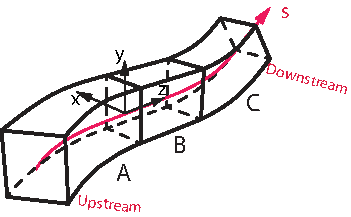
\includegraphics[width=0.6\textwidth]{figures/element-stream.pdf}
  \caption{The \vn{local} coordinate system is constructed by taking the ordered list of lattice elements and
connecting the \vn{exit} frame of one element to the \vn{entrance} frame of the next.}
  \label{f:leggo}
\end{figure}

The \vn{local} coordinate system is constructed by taking the ordered list of lattice elements and
connecting the \vn{(x, y, z)} \vn{exit} frame of one element to the \vn{(x, y, z)} \vn{entrance}
frame of the next (just like LEGO blocks). Given a line constructed as:
\begin{code}
    lat: line = (A, B, C)
\end{code}
The result could look as shown in Figure~\ref{f:leggo}. The reference trajectory is shown in
red.

%----------------------------------------------------------
\subsection{Laboratory Coordinates Relative to Global Coordinates}
\label{s:lab.rel.glob}

\begin{figure}[tb]
  \centering
  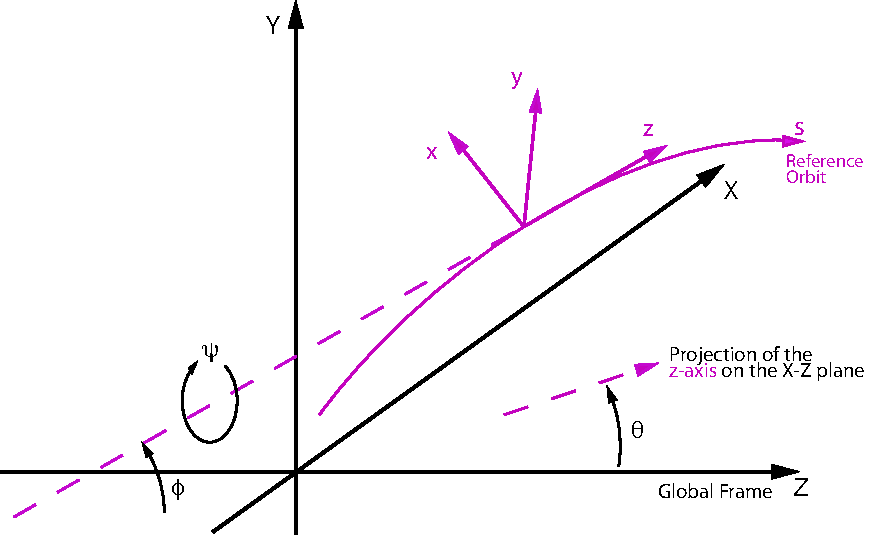
\includegraphics[width=0.9\textwidth]{figures/global-coords.pdf}
  \caption{The global coordinate system.}
  \label{f:global}
\end{figure}

For any given \vn{s}-position on the reference orbit, the \vn{local} coordinate system is described with
respect to the \vn{global} coordinate system by 6 parameters as shown in Figure~\ref{f:global}:
\vspace{-5 pt}
\begin{itemize}
\item (\vn{X}, \vn{Y}, \vn{Z}) global position
\item \vn{$\theta$} azimuth angle in the (X, Z) plane.
\item \vn{$\phi$} elevation angle
\item \vn{$\psi$} roll angle.
\end{itemize}

Notes:
\vspace{-5 pt}
\begin{itemize}
\item 
The default is for the beginning of the lattice (\vn{s} = 0) is to have the local \vn{(x, y, z)}
coordinate system aligned with the global \vn{(X, Y, Z)} coordinate system with $\theta$, $\phi$ and
$\psi$ all being zero.
\item 
For a machine that lies in the horizontal plane, the $\phi(s)$ and $\psi(s)$ angles are zero for all
\vn{s}.
\end{itemize}

%----------------------------------------------------------
\subsection{Patch Elements}
\label{s:patch}

\begin{figure}[tb]
  \centering
  \begin{subfigure}[t]{0.48\textwidth}
    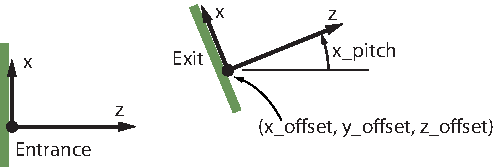
\includegraphics[width=\textwidth]{figures/patch.pdf}
    \vspace*{5pt}
    \caption{The body coordinates at the exit end of a \vn{patch} is set by the element attributes
\vn{x_offset}, \vn{y_offset}, \vn{z_offset}, \vn{x_pitch}, \vn{y_pitch}, and \vn{tilt}.}
    \label{f:patch}
  \end{subfigure}
  \hfil
  \begin{subfigure}[t]{0.48\textwidth}
    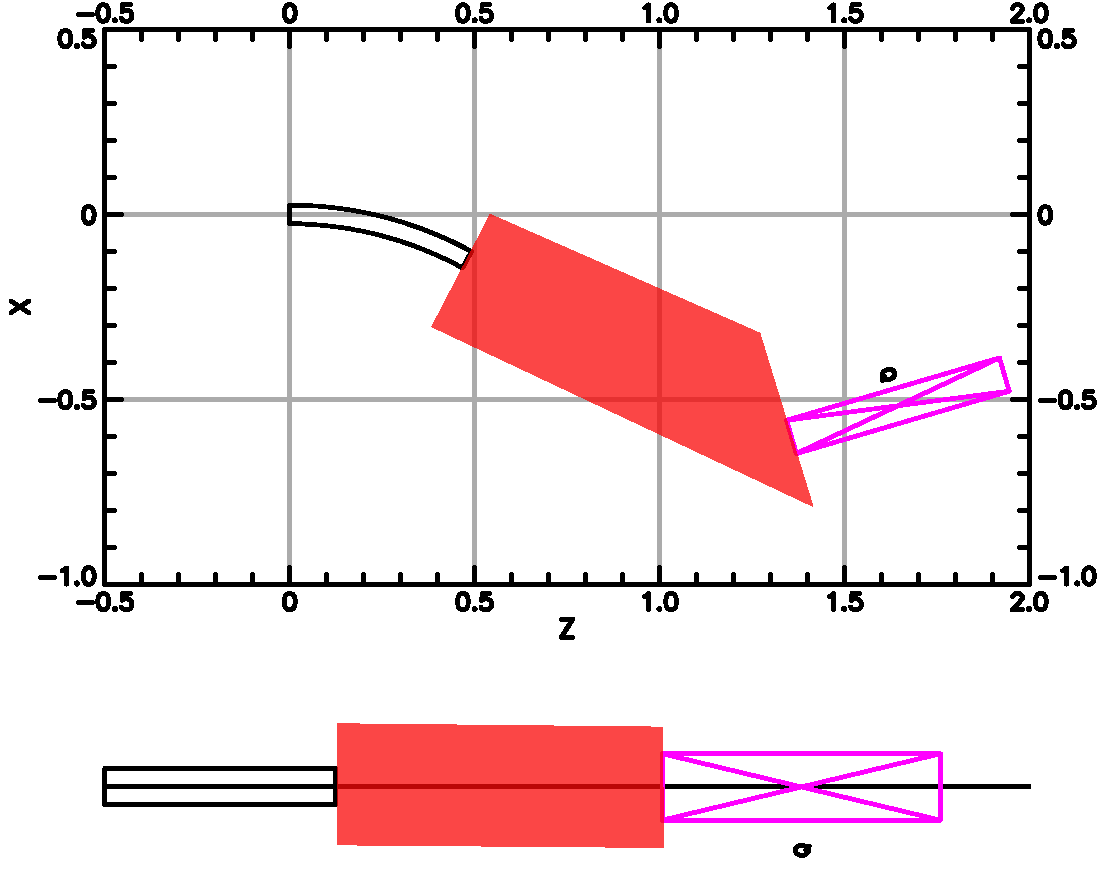
\includegraphics[width=\textwidth]{figures/patch-example.pdf}
    \caption{Lattice with a patch element.
The patch element is the coordinates patch element in a lattice. [Note: The default is not to
draw \vn{patch} elements in a \vn{floor_plan} plot.]}
    \label{f:patch.example}
  \end{subfigure}
  \caption{}
\end{figure}

\vn{Patch} elements are used to shift the reference orbit. As a consequence, the nominal placements
of all elements downstream of the patch are affected. This is useful in simulating things like injection
or extraction lines where the patch is used to reorient the reference orbit so that it follows the 
injection or extraction line.

For \vn{patch} elements the same six parameters that are used to misalign straight line elements
are, for a \vn{patch}, used to set the placement of the \vn{exit} frame relative to the \vn{entrance}
frame. The transformation from entrance coordinates to exit coordinate is:
\vspace{-5 pt}
\begin{enumerate}
\item Initially the exit coordinates coincide with the entrance coordinates.
\item The origin of the exit coordinates is translated by (\vn{x_offset}, \vn{y_offset}, \vn{z_offset})
\item The \vn{x_pitch} and \vn{y_pitch} rotations (in radians) are applied. 
The \vn{x_pitch} rotation rotates the \vn{+z} axis
towards the \vn{+x} axis (rotation around the +y axis). The \vn{y_pitch} rotation rotates the \vn{+z} axis
towards the \vn{+y} axis (rotation around the -x axis).
\item The \vn{tilt} rotation (in radians) rotates the exit coordinates around the exit coordinate's +z
axis.
\end{enumerate}
This transformation is illustrated in Figure~\ref{f:patch}. The transformation from \vn{patch}
\vn{entrance} to \vn{exit} coordinates is the same transformation from laboratory coordinates at the
center of a straight element to the element body coordinates at the center of the misaligned
element.

\subsection{Example:}
\begin{code}
! Lattice File: patch.bmad
beginning[beta_a] = 10.   ! m  a-mode beta function
beginning[beta_b] = 10.   ! m  b-mode beta function
beginning[e_tot] = 10e6   ! eV
parameter[geometry] = open  ! or closed

b: sbend, L = 0.5, g = 1    ! g = 1 / bending_radius
p: patch, z_offset = 1, x_pitch = pi/4
q: quadrupole, L = 0.6, k1 = 0.23

lat: line = (b, p, q)   ! List of lattice elements
use, lat                ! Line used to construct the lattice
\end{code}

Start \tao with the lattice file \vn{patch.bmad}. Create a
\vn{floor_plan} with the command \vn{place r11 floor}. The result is shown in
Figure~\ref{f:patch.example} except that, by default, \tao does not draw a patch element so, in the
figure, the patch has been drawn in by hand. The global coordinates of the nominal positions of the
elements can be seen by using the \vn{show lat -floor} command:
\begin{code}
Tao> show lat -floor

      Values at End of Element:
Ix  name      key               s          X         Y         Z     Theta ...
 0  BEGINNING Beginning_Ele  0.000    0.0000    0.0000    0.0000    0.0000 ...
 1  B         Sbend          0.500   -0.1224    0.0000    0.4794   -0.5000 ...
 2  P         Patch          1.207   -0.6018    0.0000    1.3570    0.2854 ...
 3  Q         Quadrupole     1.807   -0.4329    0.0000    1.9327    0.2854 ...
 4  END       Marker         1.807   -0.4329    0.0000    1.9327    0.2854 ...
\end{code}

A \vn{patch} represents a field free space so a particle traveling through a patch propagate as in a
drift. The difference is that in a \vn{patch} there is a coordinate transformation from entrance
coordinates to exit coordinates.

\subsection{Exercises:}

\begin{enumerate}[leftmargin=*]
\item
Modify the lattice file \vn{simple.bmad} to include a \vn{girder} element supporting elements \vn{B}
and \vn{Q}. Misalign the \vn{girder} and verify that a supported element will have \vn{_tot}
attributes different from the misalignment attributes.
%
\item
The \vn{show ele -floor} command will show the global coordinates of both the nominal (non-misaligned) position
as well as the misaligned (actual) position of an element. For example
\begin{code}
show ele Q -floor
\end{code}
On the \tao command line, misalign any element using the \vn{set ele} command and observe what the differences are between  the nominal and misaligned positions. Can you predict what the difference will be between the nominal and misaligned positions when you change the \vn{tilt} of \vn{Q}?
%
\item
Using lattice \vn{simple.bmad}, calculate by hand the floor coordinates at the exit end of element Q and compare this with the coordinates as calculated by Bmad.
\end{enumerate}

\newpage

%------------------------------------------------------------------------------
%------------------------------------------------------------------------------
\section{Constructing the Ring}
\label{s:ring}

%------------------------------------------------------------------------------
\subsection{Ring Construction}

\begin{figure}[h!]
  \includegraphics*[width=\columnwidth]{figures/ring}
  \caption{\label{f:ring}Mirror symmetry about the centers of each straight.}
\end{figure}

In the previous chapters, 
forward and reverse arc lines, forward and reverse straight section lines, 
and forward and reverse lines to connect the arcs to the straight sections 
(with dispersion suppression and matching the betas) were constructed. 
In this chapter, the entire ring is created based on Fig.~\ref{f:ring}. 
All that's left is a section to match the straight section to the arc, including dispersion "creation" and betas matching, as shown in Fig.~\ref{f:sextant}.
\begin{figure}[!h]
  \centering
  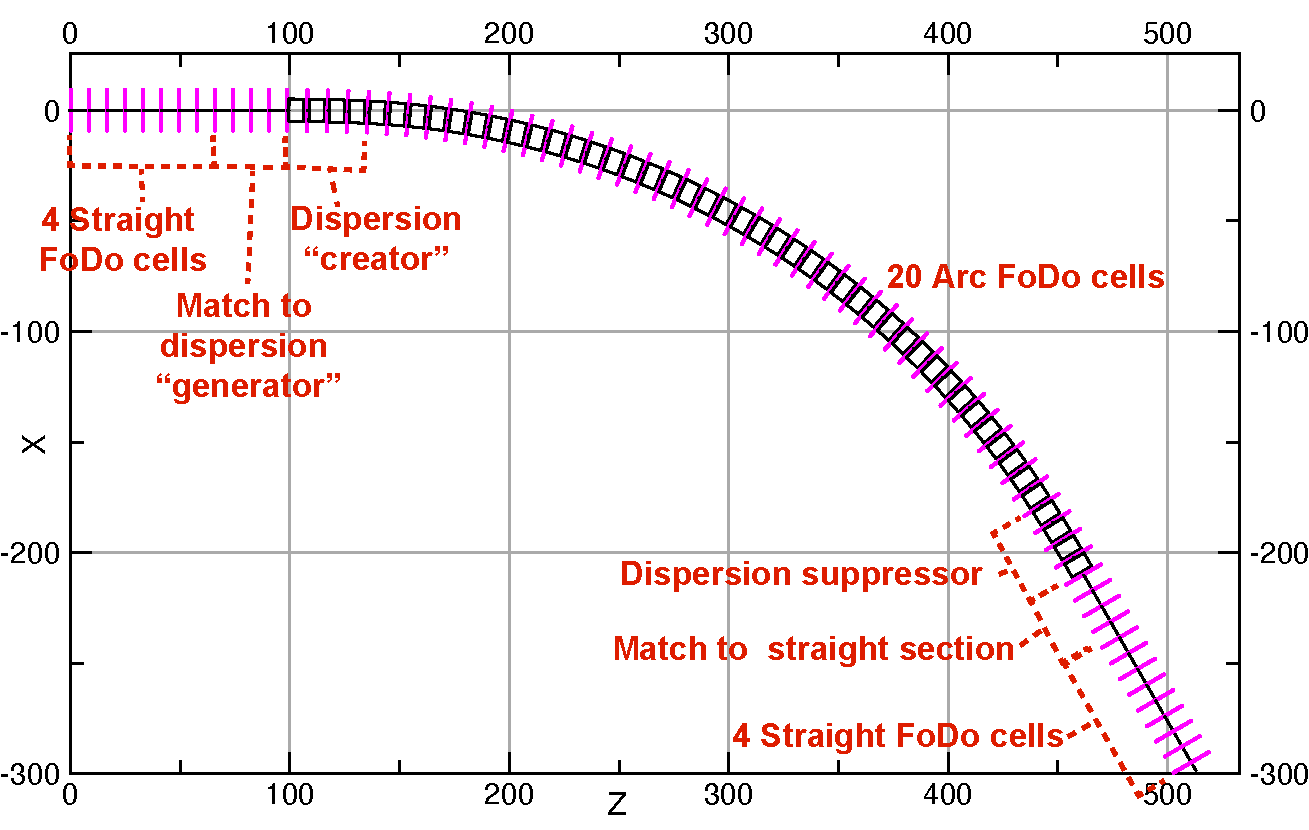
\includegraphics[width=0.8\linewidth]{figures/sextant.pdf}
  \caption{A sextant of the ring.}
  \label{f:sextant}
\end{figure}

Does this mean a dispersion "creator" for both the forward and reverse sextants needs to be created? Fortunately, no! Considering the mirror symmetry shown in Fig.~\ref{f:ring}, the quadrupole settings for the forward sextant dispersion suppression and matching are equal to the quadrupole settings for the reverse dispersion \textit{creation} and matching. Likewise, the reverse dispersion suppression and matching quadrupole settings are equal to the forward dispersion creation and matching section quadrupoles. Therefore, no optimization is necessary here. All that is needed is to 
connect the lines together.

%------------------------------------------------------------------------------
\subsection{Example: Forward Straight Section to Arc}

As an example, the forward line to connect the straight section to the arc, \vn{SS_TO_ARCF}, will be constructed. 
The example lattice file can be found in \vn{/lattices/5_Ring/}. 
Construction of \vn{SS_TO_ARCR} and the entire ring will be left as an exercise.

Following Fig.~\ref{f:sextant}, both the matching to dispersion creator line (which we'll call \vn{MDCF}), and the dispersion creator line itself (which we'll call \vn{DISPCREF}) need to be construted. Using the mirror symmetry as shown in Fig.~\ref{f:ring}, it is seen that \vn{SS_TO_ARCF} will use the same quadrupole settings as in \vn{ARC_TO_SSR}. Keeping with our convention of starting each line with a full horizontally-focusing quadrupole, this is 

\begin{code}
! Match forward straight section to dispersion "creator" (use QFR)
MDCF: line = (QFSS, D1, DB, D2, QDR3, D1, DB, D2,
              QFR3, D1, DB, D2, QDR2, D1, DB, D2) 

! Forward dispersion "creator" (use QFR)
DISPCREF: line = (QFR2, D1, BH, D2, QDR1, D1, BH, D2, 
                  QFR1, D1, BH, D2, QD, D1, BH, D2)

SS_TO_ARCF: line = (MDCF, DISPCREF)
\end{code}

After matching the straight sections to the arc, it is now time to contruct the full ring.

%------------------------------------------------------------------------------
\subsection{Exercises} 

\begin{enumerate}[leftmargin=*]
\item \textbf{Construct the reverse straight section to arc lines:} Construct \vn{SS_TO_ARCR} using the example shown above and Figs.~\ref{f:ring} and \ref{f:sextant}.
%
\item \textbf{Construct the ring}
%
\begin{enumerate}[label*=\arabic*.]
\item Gather all elements from each \textit{optimized} file
\item Gather the arc and SS FODO cells
\begin{code}
! (2): Gather arc and SS FoDo cells

! Straight section forward FoDo:
FODOSSF: line = ( QFSS, D1, DB, D2, QDSS, D1, DB, D2)

! Arc forward FoDo:
FODOAF: line = (QF, D1, B, D2, QD, D1, B, D2)

! Arc reverse FoDo:
FODOAR: line = (QF, D2, B, D1, QD, D2, B, D1)

! Straight section reverse FoDo:
FODOSSR: line = ( QFSS, D2, DB, D1, QDSS, D2, DB, D1)
\end{code}
%
\item Gather dispersion suppression and matching to SS lines (ARC\_TO\_SSF, ARC\_TO\_SSR)
\begin{code}
! (3): Gather dispersion suppression 
!      and matching to SS lines (ARC_TO_SSF, ARC_TO_SSR)

! Forward dispersion suppressor:
DISPSUPF: line = (QF, D1, BH, D2, QD, D1, BH, D2, 
                  QFF1, D1, BH, D2, QDF1, D1, BH, D2)

! Match forward dispersion suppressor to SS:
MSSF: line = ( QFF2, D1, DB, D2, QDF2, D1, DB, D2,  
               QFF3, D1, DB, D2, QDF3, D1, DB, D2)

ARC_TO_SSF: line = (DISPSUPF, MSSF)

! Reverse dispersion suppressor:
DISPSUPR: line = ( QF, D2, BH, D1, QD, D2, BH, D1, 
                   QFR1, D2, BH, D1, QDR1, D2, BH, D1)

! Match reverse dispersion suppressor to SS:
MSSR: line = ( QFR2, D2, DB, D1, QDR2, D2, DB, D1,  
               QFR3, D2, DB, D1, QDR3, D2, DB, D1)

ARC_TO_SSR: line = (DISPSUPR, MSSR)
    \end{code}
        \item Gather matching to dispersion creation and dispersion creation lines (\vn{SS_TO_ARCF}, \vn{SS_TO_ARCR}) from the Example and first exercise in this section
        \item Build the ring!
  \end{enumerate}

\end{enumerate}
\begin{code}
! (5): Build the ring!

SEXTANT1:  line = (4*FODOSSF, SS_TO_ARCF, 20*FODOAF, ARC_TO_SSF, 4*FODOSSF)
SEXTANT3:  line = (4*FODOSSR, SS_TO_ARCR, 20*FODOAR, ARC_TO_SSR, 4*FODOSSR)
SEXTANT5:  line = (4*FODOSSF, SS_TO_ARCF, 20*FODOAF, ARC_TO_SSF, 4*FODOSSF)
SEXTANT7:  line = (4*FODOSSR, SS_TO_ARCR, 20*FODOAR, ARC_TO_SSR, 4*FODOSSR)
SEXTANT9:  line = (4*FODOSSF, SS_TO_ARCF, 20*FODOAF, ARC_TO_SSF, 4*FODOSSF)
SEXTANT11: line = (4*FODOSSR, SS_TO_ARCR, 20*FODOAR, ARC_TO_SSR, 4*FODOSSR)

RING: line = (SEXTANT1, SEXTANT3, SEXTANT5, SEXTANT7, SEXTANT9, SEXTANT11)
use, RING
\end{code}

\begin{enumerate}[leftmargin=*]
\setcounter{enumi}{2}
\item \textbf{Check that the ring closes geometrically} using either \vn{show element end -floor} or \vn{show element end -all}. What is the circumference of the ring?
%
\item \textbf{Use Tao's place command} to display a \vn{floor_plan} drawing (Figs~\ref{f:ring} and \ref{f:sextant}
are \vn{floor_plan} drawings). First, use \vn{place r11 floor_plan} to place the floor template in the plot region (use \vn{show plot} to display the region). Then, try to adjust the drawing boundaries using \vn{scale}, \vn{scale all}, and \vn{x_scale all} commands.
%
\end{enumerate}

\newpage

%------------------------------------------------------------------------------
%------------------------------------------------------------------------------
\section{Low-Beta Interaction Region Insertion}

%------------------------------------------------------------------------------
\subsection{Introduction}

\marginnote{\footnotesize\hspace*{-0.6in}\parbox{1.1in}{
For IR simulations \bmad has a \vn{BeamBeam} lattice element for simulating the fully-nonlinear weak-strong beam-beam effect. \bmad also has a \vn{crab_cavity} element to simulate crabbing
with a non-zero crossing angle. Discussion of this is beyond the scope of this tutorial.
}}[-0.1in]
%
In this chapter an Interaction Region (IR) with a low beta
Interaction Point (IP)  will be constructed by modifying the 6 o'clock straight section quadrupoles
as shown in Figs.~\ref{f:sstoir}A and \ref{f:sstoir}B. 
\begin{figure}[bt]
   \centering
  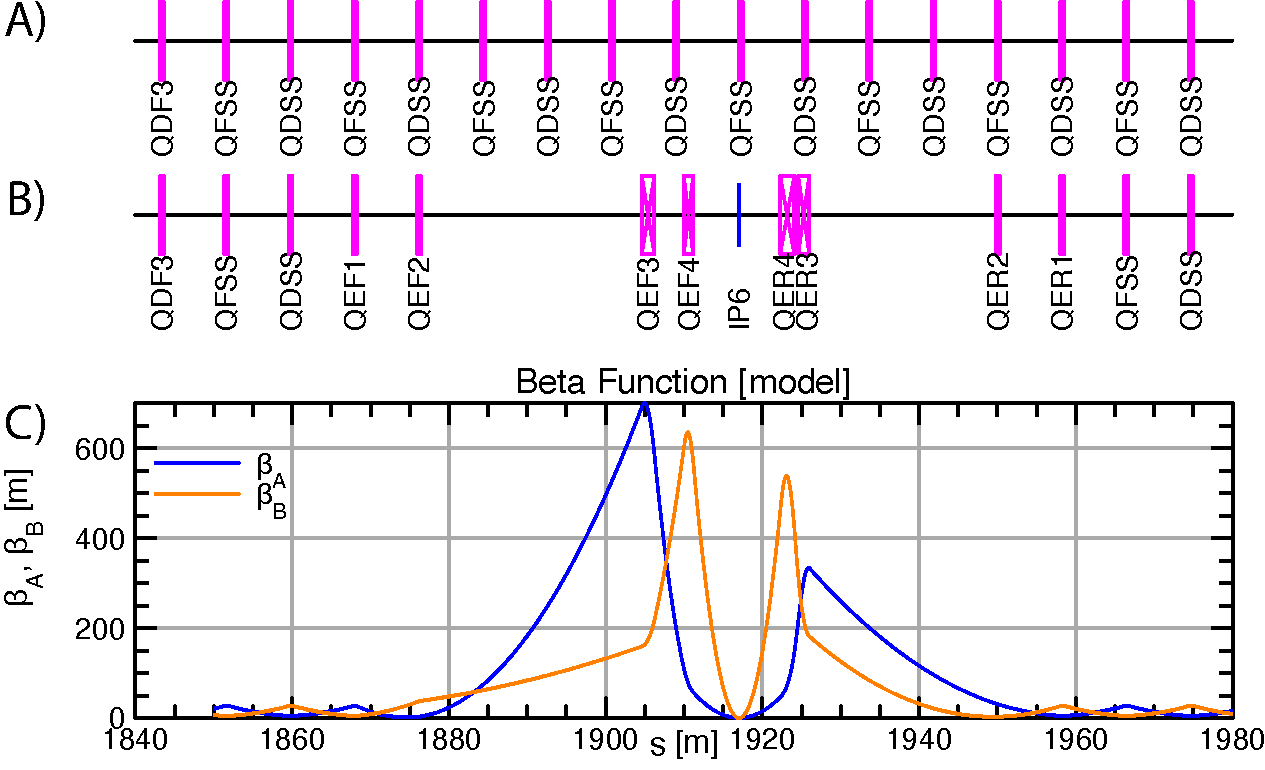
\includegraphics[width=0.9\linewidth]{figures/ip6-layout.pdf}
  \caption{A) Layout before modification. B) Layout with IR constructed. C) IR Beta functions.}
  \label{f:sstoir}
\end{figure}

\begin{figure}[bt]
  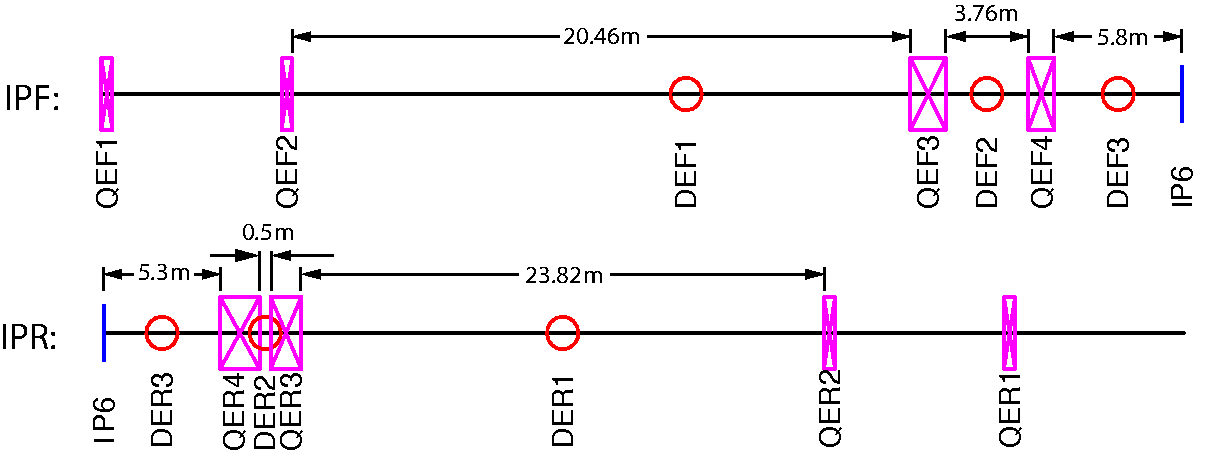
\includegraphics[width=0.9\linewidth]{figures/irspecs.PDF}
  \caption{Interaction region dimensions. Red circles mark drifts with non-standard lengths. 
  IPF: Forward section before the IP. IPR: Reverse section after the IP.}
  \label{f:ir}
\end{figure}
The IR is divided into two parts which are constructed separately as shown in Fig.~\ref{f:ir}. 
IPF is the upstream ``forward'' section before the IP (labeled IP6) and  IPR is the downstream ``reverse'' section after IP6.
At the IP, the betas are to be optimized to the values $\beta_a^*=0.6$ and $\beta_b^*=0.06$, and,
as standard for many IPs, the alpha values $\alpha_a^*$, and $\alpha_b^*$ will be optimized to zero. 
The surrounding quadrupoles will be adjusted to match these IP parameters while still matching to the periodic solution at the ends of the sections furthest from the IP. 
Because this region is particularly sensitive, this match is achieved with the following steps:
\begin{enumerate}[leftmargin=*]
\item Match the forward line from SS to IP
%
\item Match \textit{backwards} the reverse line from SS to IP
%
\item Connect the two and match the full line to the periodic solution once more to ensure a perfect match
\end{enumerate}

%------------------------------------------------------------------------------
\subsection{Example: Constructing the Upstream and Downstream IR Lines}
The example lattice file can be found in \vn{/lattices/6_IP/a_IP0/}.

Construct the upstream and downstream IR lines, shown on the top and bottom of Fig.~\ref{f:ir} respectively, and leave the upstream, downstream, and full IR matching described in the introduction as exercises.

To construct the IR lines:

\begin{enumerate}[leftmargin=*]
    \item Start with \vn{fodoSSF.bmad}, the optimized forward straight-section lattice file
    \item Set geometry to open
    \begin{code}
parameter[geometry] = open   ! (2): Set geometry to open  
    \end{code}
    \item Define forward (upstream) interaction region drifts and quads (strengths TBD, start with SS quadrupole strengths)
    \begin{code}
! (3): Define forward (upstream) interaction region drifts and 
!       quads (strengths TBD, start with SS)
QEF1: Quadrupole, L = 0.5, K1 = 0.351957452649287
QEF2: Quadrupole, L = 0.5, K1 = -0.351957452649287
DEF1: Drift, L = 20.46
QEF3: Quadrupole, L = 1.6, K1 = 0.351957452649287
DEF2: Drift, L = 3.76
QEF4: Quadrupole, L = 1.2, K1 = -0.351957452649287
DEF3: Drift, L = 5.8 
    \end{code}
    \item Define the interaction point element. Use a \vn{Marker} element for this. \vn{Markers} have zero length and have no impact on the orbit or spin transport.

    \begin{code}
! (4): Define IP
IP6: marker

    \end{code}
    \item Define reverse (downstream) interaction region drifts and quads (strengths TBD, start with SS quadrupole strengths)
    \begin{code}
! (5): Define reverse (downstream) interaction region drifts and 
!       quads (strengths TBD, start with SS)
DER3: Drift, L = 5.3
QER4: Quadrupole, L = 1.8, K1=-0.351957452649287
DER2: Drift, L = 0.5
QER3: Quadrupole, L = 1.4, K1=0.351957452649287
DER1: Drift, L = 23.82
QER2: Quadrupole, L = 0.5, K1 = 0.351957452649287
QER1: Quadrupole, L = 0.5, K1 =-0.351957452649287
    \end{code}
    \item Define the upstream and downstream lines
        \begin{code}
! (6): Define the upstream and downstream lines
IPF: line = ( QEF1, D1, DB, D2, QEF2, D1, DB, 
              D2, DEF1, QEF3, DEF2, QEF4, DEF3, IP6)
IPR: line = (IP6, DER3, QER4, DER2, QER3, DER1,
             QER2, D2, DB, D1, QER1, D2, DB, D1)
    \end{code}
\end{enumerate}

After defining the two IP lines, the exercises will focus on region matching and optimization of our updated ring. 
%------------------------------------------------------------------------------
\subsection{Exercises}

\begin{enumerate}[leftmargin=*]
%
\item {\bf Forward (upstream) interaction region matching:} Using the \vn{IPF} line defined above, vary \vn{QEF1}, \vn{QEF2}, \vn{QEF3}, and \vn{QEF4} so that at \vn{IP6} $\beta_a=0.6$, $\beta_b=0.06$, $\alpha_a=\alpha_b=0$. After optimizing, instead of \vn{write}-ing the lattice, make a copy of the \vn{var1.out} file and rename it to something like \vn{IPF.out}. This output file is a Bmad lattice file that sets the quadrupoles to their correct strengths.
%
\item {\bf Reverse (downstream) interaction region matching:} Match \textit{backwards} the downstream interaction region line \vn{IPR} defined above, starting from the end of the line and ending at the interaction point, varying \vn{QER1}, \vn{QER2}, \vn{QER3}, and \vn{QER4} that $\beta_a=0.6$, $\beta_b=0.06$, $\alpha_a=\alpha_b=0$ at \vn{IP6}. Once again, save a copy of the final \vn{var1.out} file containing the optimized quadrupole strengths and rename it to something like \vn{IPR.out}. Hint: the line can be reflected using a negative sign:
\begin{code}
IPR_reflected: line = (-IPR)
\end{code}
%
\item {\bf Call command:} The optimized quadrupole settings in the \vn{.out} files obtained above can be called directly in the lattice file using the \vn{call} command at the end of the lattice file. \bmad will read in the entire lattice file, and then set the quadrupole strengths accordingly. E.g., at the end of the lattice file:
\begin{code}
! Define and use IP line
IP: line = (IPF,IPR)
use, IP

! Call the quadrupole settings in IPF.out and IPR.out
call, file = "IPF.out"
call, file = "IPR.out"
\end{code}
This should give a very good match, however to ensure a perfect solution, the full line to the periodic solution is matched once more. Using the full IR line (\vn{(IPF, IPR)}) now, vary the downstream quadrupoles \vn{QER1}, \vn{QER2}, \vn{QER3}, and \vn{QER4} to match perfectly to the periodic betas in the straight section at the end of the line. Now you can use \vn{write bmad IP.bmad} with the fully optimized IR quadrupole settings
%
\item {\bf Add the IR into the ring:} Copy the optimized lattice elements from \vn{IP.bmad} into the ring lattice file, copy the \vn{IPF} and \vn{IPR} lines into the ring lattice file, and finally add the IP into the ring by modifying \vn{SEXTANT5} and \vn{SEXTANT7}:
\begin{code}
SEXTANT5: line = (4*FODOSSF, SS_TO_ARCF, 20*FODOAF, ARC_TO_SSF, FODOSSF, IPF)
SEXTANT7: line = (IPR, FODOSSR, SS_TO_ARCR, 20*FODOAR, ARC_TO_SSR, 4*FODOSSR)
\end{code}
%
\item \textbf{Alpha and Beta Functions:} How should you change the initial betas and alphas for a proper match using the reflected line?
Hint: the betas and alphas are the same as calculated in earlier chapters.
%
\item \textbf{Importance of variable step size:}
In Exercise 1, you optimized the match the IP Twiss using a 
\vn{step} size for varying the quadrupole \vn{k1} values of $10^{-6}$.
How is this step size used with the Levenberg-Marquardt optimization?
Verify that if, instead, a step size of $10^{-4}$ is used the optimization does not
converge to a usable solution. Why is this?
%
\end{enumerate}

\newpage

%------------------------------------------------------------------------------
%------------------------------------------------------------------------------
\section{Tune Cell}

%------------------------------------------------------------------------------
\subsection{Introduction}

In order to adjust the tune of the ring, the phase advance per FODO cell in one of the straight sections can be adjusted, while ensuring it is still matching to the periodic solution in each of the surrounding arcs. We'll put this ``tune cell'' in the 2 o'clock straight section, and modify the lines/lattice elements by simply appending a \vn{_2} to the names.

Required for the optimization is:
\begin{enumerate}[leftmargin=*]
    \item Setting the phase advances in the FODOSSF/FODOSSR straight section for desired tunes $Q_x=54.08$ and $Q_y=54.14$ (2 constraints)
    \item Matching from the dispersion suppressor to the new periodic betas and alphas in the center FODOSSF/FODOSSR section (4 constraints)
    \item Matching the center FODOSSF/FODOSSR section to the dispersion creator (would be 4 constraints but these are defined already by the mirror symmetry)
\end{enumerate}

These 6 constraints can be satisfied using the four quadrupoles in the forward matching to SS (\vn{QFF2_2}, \vn{QDF2_2}, \vn{QFF3_2}, and \vn{QDF3_2}), and the two quadrupoles in the straight section (\vn{QFSS_2} and \vn{QDSS_2}). 

\begin{figure}[!h]
    \centering
    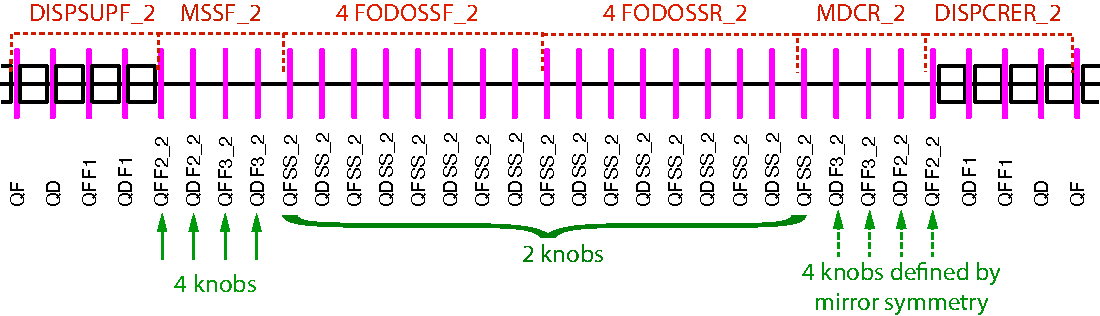
\includegraphics[width=1\linewidth]{figures/tunecell.pdf}
    \caption{Enter Caption}
    \label{f:tunecell}
\end{figure}

%------------------------------------------------------------------------------
\subsection{Example: tao.init for the Tune Cell}

The example file can be found at \vn{/lattices/7_TuneCell/tao.init}.

To define datums that constrain the solution to have periodic betas in the straight section,
\vn{expression} datums are used. Expressions are an extremely powerful tool that allows for complex lattice optimizations and matching techniques. 

In this case, required is that the betas at one focusing quadrupole in the center FODO cells are equal to the betas at the next focusing quadrupole. Equivalently, required is that the difference of those two are equal to zero.
The appropriate datums are 
\begin{code}
! Require periodic betas in center FoDo cells of 2 o'clock tune cell
datum(1) = 'expression: lat::beta.a[QFSS_2##4] - lat::beta.a[QFSS_2##5]' 
                                                  '' '0' 'end' 'target' 0 10
datum(2) = 'expression: lat::beta.b[QFSS_2##4] - lat::beta.b[QFSS_2##5]' 
                                                  '' '0' 'end' 'target' 0 10
datum(3) = 'expression: lat::alpha.a[QFSS_2##4] - lat::alpha.a[QFSS_2##5]' 
                                                   '' '0' 'end' 'target' 0 10
datum(4) = 'expression: lat::alpha.b[QFSS_2##4] - lat::alpha.b[QFSS_2##5]' 
                                                   '' '0' 'end' 'target' 0 10
\end{code}

The syntax \vn{lat::beta.a[QFSS_2\#\#4]} evaluates to the value of the \vn{a}-mode beta function at the fourth lattice element named \vn{QFSS_2}.
The above datums have a \vn{measured} (target) value of zero so that the contribution to the merit function
will be zero when the differences of the betas at the fourth \vn{QFSS_2} and at the fifth \vn{QFSS_2} are zero.
Thais in, when they are equal. This ensures periodicity in the optics in the straight section.

Besides the above datums, other datums are need to make sure that the outgoing Twiss from the modified straight section correctly match the Twiss at the start of the dispersion creator \vn{DISPCRER_2} (see Fig.~\ref{f:tunecell}. The needed datums are:
\begin{code}
! Match betas to dispersion creator after tune cell
datum(5) = 'beta.a' '' '' 'QFF2_2##2' 'target' 30.6104309489717465  10
datum(6) = 'beta.b' '' '' 'QFF2_2##2' 'target'  5.56679467017438689 10
datum(7) = 'alpha.a' '' '' 'QFF2_2##2' 'target' 2.40115683012980607 100
datum(8) = 'alpha.b' '' '' 'QFF2_2##2' 'target'   -.47804044385806721 100
\end{code}

Finally, datums are needed to set the optimized tune to the desired values:
\begin{code}
! Set phase advance to nearest desired fractional tunes (54.08, 54.14)
datum(9) = 'phase.a' '' '' 'end' 'target' 339.79466141227203 10
datum(10) = 'phase.b' '' '' 'end' 'target' 340.17165253070283 10
\end{code}

%------------------------------------------------------------------------------
\subsection{Exercises}

\begin{enumerate}[leftmargin=*]
    \item {\bf Implement the tune cell:} Add the new special quadrupoles shown in Fig.~\ref{f:tunecell}, and optimize them using the \vn{tao.init} file created in the example so the lattice has the correct tunes $Q_x=54.08$ and $Q_y=54.14$.
\end{enumerate}

%The syntax \vn{QFSS_2##4} refers to the fourth element in the lattice which has the name \vn{QFSS_2}. Because we are adding 8 special FODO cells into the straight section, this refers to the center-left focusing quadrupole, and \vn{QFSS_2##5} refers to the center-right focusing quadrupole in the straight section. 

\newpage

%------------------------------------------------------------------------------
%----------------------------------------------------------
\section{Particle Phase Space Coordinates}
\label{s:phase.space}

%------------------------------------------------------------------------------
\subsection{Phase Space}

\begin{figure}[tb]
  \centering
  \begin{subfigure}[t]{0.48\textwidth}
    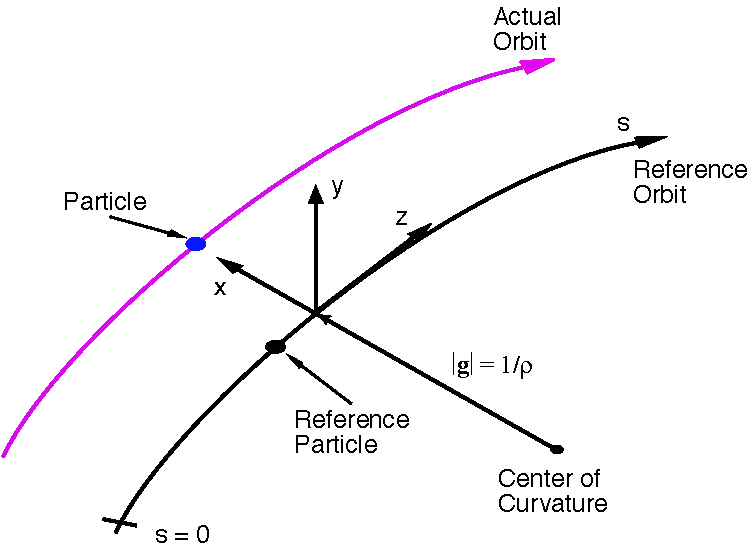
\includegraphics[width=0.9\textwidth]{figures/local-coords.pdf}
    \caption{Particle coordinate positions are relative to the reference orbit.}
    \label{f:part.coords}
  \end{subfigure}
  \hfil
  \begin{subfigure}[t]{0.48\textwidth}
    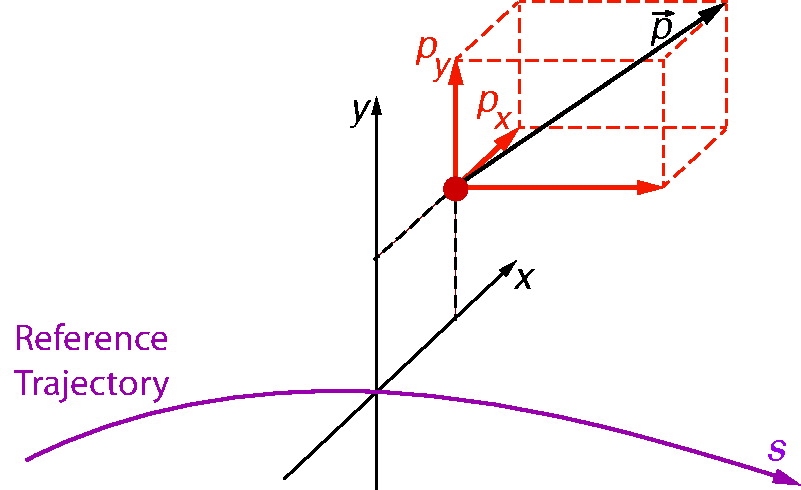
\includegraphics[width=\textwidth]{figures/CoordinateSystem1.pdf}
    \caption{Particle phase space.}
    \label{f:phase.space}
  \end{subfigure}
  \caption{}
\end{figure}

Figure~\ref{f:part.coords} shows the reference orbit (laboratory coordinate system) which was
discussed in chapter~\ref{s:coords}. The
reference coordinates $(x, y, z)$ associated with a given point a distance $s$ along the reference
point has the coordinate origin at the given point and the $z$-axis tangent to the reference orbit.

A particle being simulated has its own trajectory as shown in the figure. Given a particle at some
point on its trajectory (blue dot in Figure~\ref{f:part.coords}), there is a point at position
\vn{s} on the reference orbit such that the $z$ coordinate of the particle is zero in the (\vn{x},
\vn{y}, \vn{z}) coordinate frame associated with the reference orbit point.

With this, the particle's position and momentum \vn{P} can be described using the coordinates:
\begin{code}
    (x(s), y(s), Px(s), Py(s), Pz(s), t(s))
\end{code}
where \vn{t(s)} is the time that the particle is at the given point. From now on, to simplify the
notation, the \vn{s} dependence will be dropped.

For tracking purposes, canonical phase space coordinates are used with the convention that upper
case \vn{P} denotes (unnormalized) momentum (Figure~\ref{f:phase.space}) and lower case \vn{p}
denotes phase space momentum. The phase space coordinates are denoted
\begin{code}
    (x, px, y, py, z, pz)
\end{code}
where
\begin{lstlisting}[mathescape]
    px = Px / P0
    py = Py / P0
    pz = (P - P0) / P0
    z  = c * @!\textbeta!@ * (t_ref - t)
\end{lstlisting}
with
\vspace{-5 pt}
\begin{itemize}
\item \vn{P0} is the reference momentum. See section~\sref{s:ref.energy}.
\item \vn{c * \textbeta} is the velocity of the particle, 
\item \vn{t_ref(s)} is the time the reference particle reaches the point \vn{s}. The reference
particle is a fictitious particle that can be imagined to be traveling on the reference orbit.
Frequently, this reference particle is thought of as describing the center of a bunch of particles.
\end{itemize}
Notes:
\vspace{-5 pt}
\begin{itemize}
\item
Do not confuse the canonical \vn{z} coordinate with the \vn{z} coordinate of the particle in the
(\vn{x},~\vn{y},~\vn{z}) coordinate frame. By construction, the latter is always zero.
\item 
For a bunch of particles at a given \vn{s} position, in general, the particles will have differing
time \vn{t}.
\item 
If the reference particle has the same {\textbeta} value as a particle, canonical \vn{z} will be the
longitudinal distance the particle is with respect to the reference particle. Positive \vn{z}
indicates that the particle is in front of the reference particle and vice versa.
\end{itemize}


\begin{figure}[tb]
  \centering
  \begin{subfigure}[t]{0.49\textwidth}
    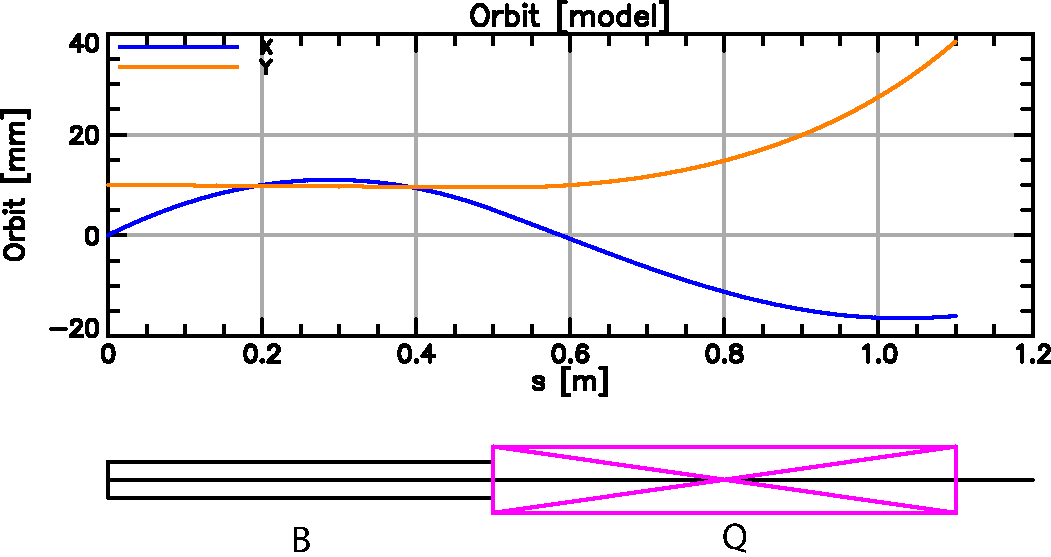
\includegraphics[width=\textwidth]{figures/phase0.pdf}
    \caption{Initial orbit.}
    \label{f:phase0}
  \end{subfigure}
  \hfil
  \begin{subfigure}[t]{0.49\textwidth}
    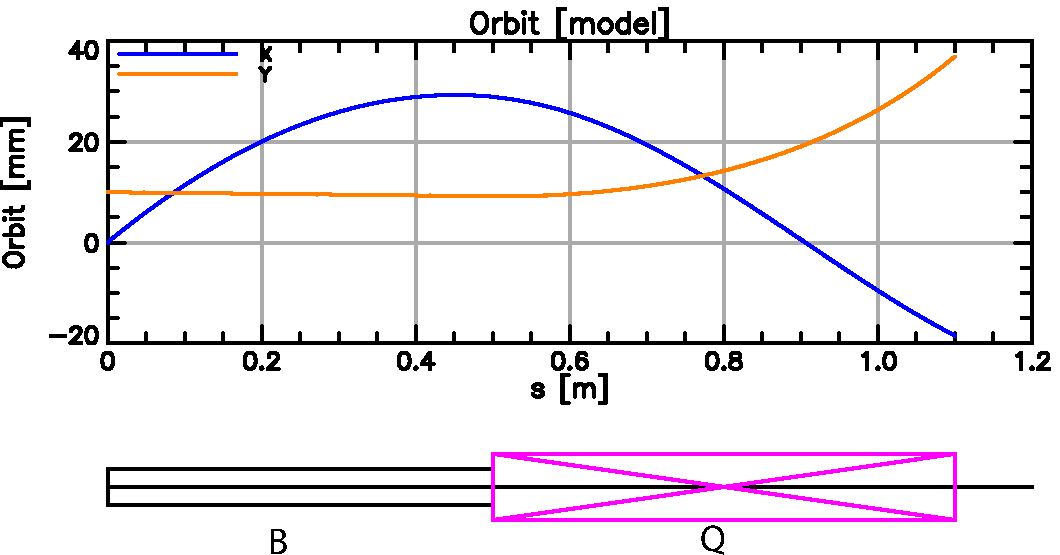
\includegraphics[width=\textwidth]{figures/phase1.pdf}
    \caption{Orbit after adjusting the starting \vn{px} phase space coordinate.}
    \label{f:phase1}
  \end{subfigure}
  \caption{}
\end{figure}

%----------------------------------------------------------
\subsection{Example}

Example lattice:
\begin{code}
! Lattice File: orbit.bmad
beginning[beta_a] = 10.   ! m  a-mode beta function
beginning[beta_b] = 10.   ! m  b-mode beta function
beginning[e_tot] = 10e6   ! eV
parameter[geometry] = open  ! or closed
bmad_com[spin_tracking_on] = T

particle_start[y] = 0.01
particle_start[px] = 0.06
particle_start[pz] = -0.2
particle_start[spin_x] = 1

b: sbend, L = 0.5, g = 1    ! g = 1 / bending_radius
q: quadrupole, L = 0.6, k1 = 10

lat: line = (b, q)      ! List of lattice elements
use, lat                ! Line used to construct the lattice
\end{code}

Start \tao with the lattice file \vn{orbit.bmad}.
Spin tracking is on (\vn{bmad_com[spin_tracking_on]} set to True) and a non-zero initial orbit is set
using \vn{particle_start} parameters. The resulting orbit is shown in Figure~\ref{f:phase0}.

The initial phase space coordinates can now be varied using the \vn{change} or \vn{set}
commands. For example:
\begin{code}
Tao> change particle_start px 0.04
           Old           New    Old-Design    New-Design         Delta
      0.060000      0.100000      0.000000      0.040000      0.040000  
\end{code}

The result is shown in Figure~\ref{f:phase1}. 

View Orbits with \vn{show lattice} command

\begin{code}
Tao> show lat -spin -orbit
      Values at End of Element:
 Index  name      key           ...           orbit  ...          spin 
                                ...               x  ...             x 
     0  BEGINNING Beginning_Ele ...    0.000000E+00  ...  0.000000E+00 
     1  B         Sbend         ...    5.027722E-03  ... -1.414516E-01 
     2  Q         Quadrupole    ...   -1.599068E-02  ... -7.350543E-02 
     3  END       Marker        ...   -1.599068E-02  ... -7.350543E-02 
\end{code}

or the \vn{show element} command

\begin{code}
Tao> show ele 1
 Element #                1
 Element Name: B
... etc...

Orbit:  Positron   State: Alive
         Position[mm] Momentum[mrad]        Spin   |
  X:       5.02772161   -44.34051580  -0.14145163  | Particle [sec]:     ...
  Y:       9.52710654    -1.27804602  -0.00171549  | Part-Ref [sec]:     ...
  Z:      -4.78648430  -200.00000000   0.98994368  | (Ref-Part)*Vel [m]: ...
\end{code}

%Add a conclusion and exercises to this part of the chapter

%------------------------------------------------------------------------------
\subsection{Exercises:}

\begin{enumerate}[leftmargin=*]
\item {\bf Phase Space:} Construct a lattice with a single drift of 2 meters length.
Set the particle species to be protons with a reference energy of $10^12$~eV (so the approximation
that the particle velocity is speed of light can be made), and
Set the initial particle position to have $p_x = 0.2$, $p_z = 1$ with all other coordinates
zero. Calculate from first principles what the phase space coordinates will be at the end of the
lattice and check that your answer agrees with \bmad.
\end{enumerate}

\newpage

%------------------------------------------------------------------------------
%------------------------------------------------------------------------------
\section{RF Cavities}
\label{s:rf}

%------------------------------------------------------------------------------
\subsection{Reference Energy and the Lcavity and RFcavity Elements}
\label{s:ref.energy}

%----------------------------------------------------------

\begin{description}[labelindent=-17pt,leftmargin=0pt]
\item[Reference Energy] \Newline
Every lattice element has a reference particle, a reference energy called \vn{E_tot}, and a
reference momentum named \vn{p0c} (in eV). The three are interrelated so knowing the reference
particle and either the reference momentum or energy, the third quantity can be calculated. The
reference momentum is used for normalization of the phase space momentum
as well as normalized strength parameters. 

For example, for a quadrupole element, the
\vn{b1_gradient} parameter (units: Tesla/m) can be used to specify the linear field gradient and the
\vn{k1} parameter (units: 1/m$^2$) is the normalized field gradient normalized using the value of
the reference momentum as discussed in the ``\vn{Magnetostatic Multipole Fields}'' section of the
``\vn{Electromagnetic Fields}'' chapter of the \bmad manual.
%
\item[Lcavity] \Newline
 \vn{Lcavity} elements are exceptions for lattices with an \vn{open} geometry, where the reference energy/momentum at the beginning of the lattice is what is set in the lattice file. Usually, the reference energy/momentum for a downsteam element inherits the reference energy/momentum of the element just upstream. 

\vn{Lcavity} elements represent an RF cavity where the reference energy/momentum at the exit end of the \vn{lcavity} is set so that a particle entering the cavity with zero phase space coordinates leaves with zero phase space coordinates. In particular, its phase space \vn{pz} will be zero at the exit end.  \vn{Lcavity} elements also have \vn{p0c_start} and \vn{E_tot_start} parameters
that are set to the reference energy of the upstream element. 
%
\item[Rfcavity] \Newline 
\vn{Rfcavity} elements also represent an RF cavity, but their reference energy/momentum is the same as the upstream element.
\end{description}

%----------------------------------------------------------
\subsection{Example: Cavity Element}

\begin{code}
! Lattice File: cavity.bmad
beginning[beta_a] = 10.   ! m  a-mode beta function
beginning[beta_b] = 10.   ! m  b-mode beta function
beginning[p0c] = 1e8   ! eV  

parameter[geometry] = open      ! or closed
parameter[particle] = He+ 

q1: quad, l = 0.1, k1 = 0.14
q2: quad, l = 0.1, b1_gradient = parameter[p0c] * q1[k1] / c_light
lc: lcavity, l = 1, voltage = 10e8, rf_frequency = 1e9
rf: rfcavity, l = 1, voltage = 10e8, phi0 = 0.25

lat: line = (q1, q2, lc, q1, q2, rf)
use, lat
\end{code}

Notes:
\vspace{-5 pt}
\begin{itemize}
\item For a \vn{lcavity} phi0 = 0 corresponds to peak acceleration.
\item For an \vn{rfcavity} phi0 = 0.25 corresponds to peak acceleration.
\end{itemize}

Start \tao as explained in with the lattice file
\vn{cavity.bmad}. Examining the \vn{lcavity} element shows:
\begin{code}
> tao -lat cavity.bmad

Tao> show ele 3
Element #                3
Element Name: LC
Key: Lcavity
... etc...
   51   P0C_START    =  1.000000E+08 eV        BETA_START   =  0.02681151
   52   E_TOT_START  =  3.729740E+09 eV        DELTA_E      =  1.000000E+09 eV
   53   P0C          =  2.910237E+09 eV        BETA         =  0.61530588
   54   E_TOT        =  4.729740E+09 eV        GAMMA        =  1.268571E+00
... etc...    
Orbit:  He+   State: Alive
         Position[mm] Momentum[mrad]        Spin   |
  X:       0.00000000     0.00000000               | Particle [sec]:     ...
  Y:       0.00000000     0.00000000               | Part-Ref [sec]:     ...
  Z:      -0.00000000     0.00000000               | (Ref-Part)*Vel [m]: ...
\end{code}

The reference energy at the start of the element, \vn{E_tot_start}, is not the same as the reference
energy at the end of the element \vn{E_tot}. The particle orbit, which started out with zero phase
space coordinates (there were no \vn{particle_start} statements to give a non-zero starting orbit), still
has zero phase space coordinates at the end of the \vn{lcavity} element.


Compare this to the \vn{rfcavity} element:
\begin{code}
Tao> show ele 6
Element #                6
Element Name: RF
Key: RFcavity
... etc...
   53   P0C         =  2.9102374E+09 eV         BETA      =  0.615305883
   54   E_TOT       =  4.7297409E+09 eV         GAMMA     =  1.2685712E+00
... etc...
 Orbit:  He+   State: Alive
         Position[mm] Momentum[mrad]        Spin   |
  X:       0.00000000     0.00000000               | Particle [sec]:     ...
  Y:       0.00000000     0.00000000               | Part-Ref [sec]:     ...
  Z:     140.37425587   494.97867675               | (Ref-Part)*Vel [m]: ...
\end{code}

Here there is no \vn{E_tot_start} parameter since the ending reference energy is always equal to the
starting one. Here, the \vn{pz} coordinate at the end of the element is nonzero.

%------------------------------------------------------------------------------
\subsection{Adding RF Cavities}

The example files for this section can be found at \vn{/lattices/9_RF/AddingRF/}

In a real machine, electrons emit synchrotron radiation as they bend around the ring, so we need to replenish the energy with an RF system. Let’s put RF cavities in the 10 o’clock straight section of our ring. We will design a special FODO cellwith RF cavities \vn{FODORF} and replace 4 FODO cells in the 10 o’clock straight section. 

In the ESR, there are two RF cavities of length $4.017 \textrm{m}$ between each quadrupole with equal drift spaces between each element. We will follow these dimensions as shown in Fig.~\ref{f:fodorf}.

\begin{figure}[!h]
  \centering
  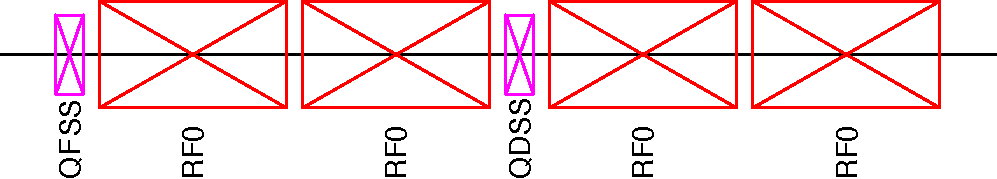
\includegraphics[width=0.9\linewidth]{figures/rf.pdf}
  \caption{FODO cell with RF cavities.}
  \label{f:fodorf}
\end{figure}

%------------------------------------------------------------------------------
\subsection{Example: Consturcting the FODO cell with RF cavities}

\begin{enumerate}[leftmargin=*]
    \item Define RF cavities and drift elements. The appropriate drift length is calculated using an expression.
    \begin{code}
RF0: RFCavity, L = 4.017, harmon = 7560,
        voltage=68.0/18.0 * 1e6 ! Start with ESR voltage
DRF: Drift, L = ((1.241+5.855+0.609)-2*4.017)/3
    \end{code}
    
    \item Define the \vn{FODORF} cell.
    \begin{code}
FODORF: line = (QFSS, DRF, RF0, DRF, RF0, DRF, QDSS, DRF, RF0, DRF, RF0, DRF)
    \end{code}
    
    \item Replace 4 FODO cells in the 10 o'clock section with \vn{FODORF} by modifying \vn{SEXTANT9} and \vn{SEXTANT9}:
    \begin{code}
SEXTANT9:  line = (4*FODOSSF, SS_TO_ARCF, 20*FODOAF, 
                              ARC_TO_SSF, 2*FODOSSF, 2*FODORF)
SEXTANT11: line = (2*FODORF, 2*FODOSSR, SS_TO_ARCR, 
                        20*FODOAR, ARC_TO_SSR, 4*FODOSSR)
    \end{code}
\end{enumerate}

%------------------------------------------------------------------------------
\subsection{Exercises}

\begin{enumerate}[leftmargin=*]
%
\item {\bf Set the synchrotron tune:} The synchrotron tune can be set by using the \vn{set z_tune} command in \tao, which varies the RF cavity voltages. Set the synchrotron tune to 0.05 and write down the new RF voltage. Add it to the end of the lattice file as
\begin{code}
RF0[voltage] = your_voltage
\end{code}
%
\item 
Modify the \vn{lcavity} in the \vn{cavity.bmad} to have a small length (so the transit time is
small), and set the beginning momentum small enough so the relativistic beta is significantly than
one. Starting the particle with a finite $z$, calculate the ending $z$ after the cavity and verity
that the cange in $z$ is consistent with the equation for $z$ given in \sref{s:phase.space.sub}.
%
\item
\vn{Lcavity} elements have an attribute \vn{phi0_err} which varies the RF phase that a particle sees
but does not change the reference energy. Add a finite \vn{phi0_err} to the \vn{cavity} element and
verify that the reference energy does not change but that the phase space \vn{pz} of the particle
(which is the normalized momentum deviation from the reference \sref{s:phase.space.sub}) does
change. With the \vn{cavity.bmad} lattice, there is a range of values for \vn{phi0_err} where the
cavity will decellerate the particle enough so that the particle will turn around and not make
it through the cavity. Approximately what is this range?
%
\end{enumerate}

\newpage

%------------------------------------------------------------------------------
%------------------------------------------------------------------------------
\section{Introduction to Long Term Tracking}

Up to this point, only the \tao program in the Bmad ecosystem has been used and tracking has implicitly been limited to tracking
a single particle once through the lattice (which is needed for computation of the Twiss functions and closed orbit \sref{s:orbit}.).
\bmad also supports multi-particle (beam) tracking and a \bmad based program, if appropriately configured, 
can track beams over an arbitrary number of turns. 
\tao is equipped to do beam tracking but \tao is not designed for tracking beams over many turns in a ring. 
Rather, the \bmad based program \ltt is designed for this. 
The \ltt program can simulate such things as misalignments, wake fields, higher order mode cavity resonances, spin polarization, energy ramping, etc. The \ltt program is also capable of simulating beam injection into and extraction 
out of a storage ring including tracking the beam through the transfer lines.

%------------------------------------------------------------------------------
\subsection{Initializing a Beam}

\bmad has two ways to define an initial beam distribution. One is providing a file containing individual particle positions. The other is using a \vn{beam_init_struct structure} which holds parameters to initialize a beam. This is discused in detail
in the \bmad manual.

\bmad accepts two file formats for beam initialization: \vn{ASCII} and \vn{HDF5}. 
HDF5 is a widely used binary format which is useful when storing beams with a large number of particles.
In this tutorial The ASCII format is used. 
The ASCII beam format describes a single bunch using a \vn{header} section followed by a \vn{table} section. Multiple bunches can be defined using multiple header/table pairs. The header lines start with a “\#” sign and contains global parameters and custom parameters. Any line in the header that does not contain a valid parameter is ignored. The last line in the header starts with “\#!” and defines the table columns. The table section follows the header section. Each row gives the parameters for one particle in the bunch.

Here is a simple beam initialization file \vn{beam.bmad}. It defines 7 electrons with various $z$ and $pz$ values.
\begin{code}
# This is the header section
# You can define parameters for all particles in the bunch
# species = electron
# charge  = 1.6e-19
# state   = alive
# Or custom parameters not used by Bmad like
# version = 1.0.0

#! x   px   y   py   z     pz    
   0   0    0   0    0     0     
   0   0    0   0    0.1   0     
   0   0    0   0    0.15  0     
   0   0    0   0    0     -0.01 
   0   0    0   0    0     0.015 
   0   0    0   0    0     0.02  
   0   0    0   0    0     0.03  
\end{code}

\begin{figure}[t]
    \centering
    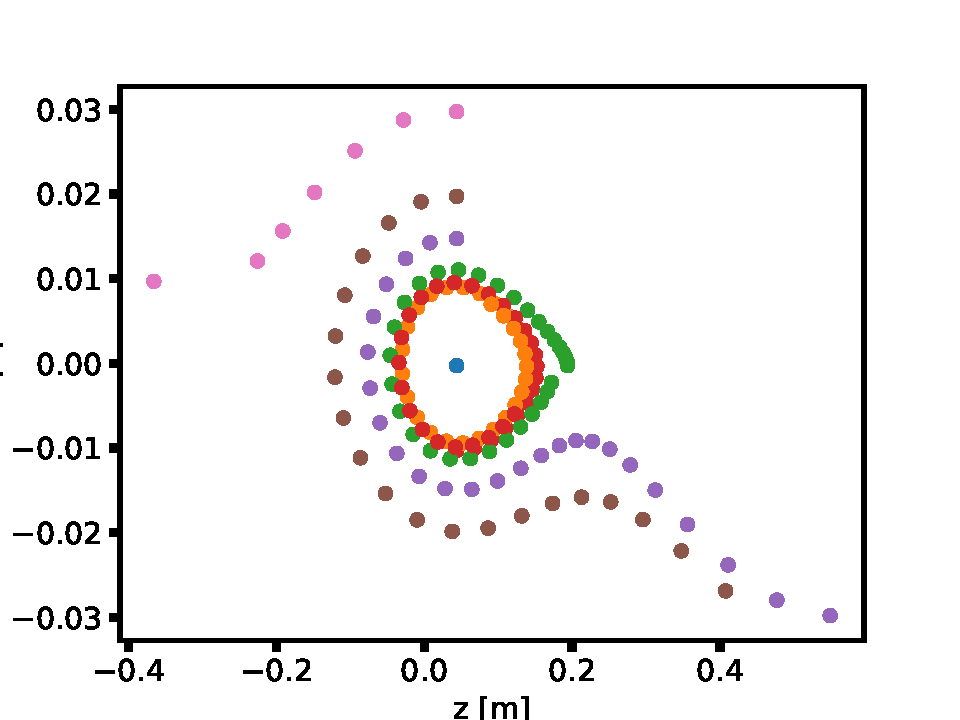
\includegraphics[width=0.8\linewidth]{figures/ltt.pdf}
    \caption{The trajectory of 7 particles in the z-pz plane over 30 turns.}
    \label{f:ltt}
\end{figure}

%------------------------------------------------------------------------------
\subsection{Initializing long term tracking}
\ltt takes an input file that defines parameters in a namelist, similar to how \tao is initialized with a \vn{tao.init} file. 
A full list of parameters and their descriptions can be found in the \ltt manual.
A simple  \vn{long_term_tracking.init} file:
\begin{code}
&params
  ltt%lat_file = "ring.bmad"
  ltt%simulation_mode = "BEAM"
  ltt%tracking_method = "BMAD"
  ltt%n_turns = 30
  ltt%particle_output_every_n_turns = 1
  ltt%phase_space_output_file = "turn"

  beam_init%center = 0, 0, 0, 0, 0, 0
  beam_init%position_file = "beam.bmad"
/
\end{code}

The \vn{long_term_tracking.init} file specifies the lattice file name, tracking method, initial beam positions, and program outputs. In this case, \ltt will track the initial beam for 30 turns and output the particle positions at the end of each turn.

You can run \ltt with this initialization file by the command \vn{long_term_tracking <ini_file>} where \vn{<ini_file>} is the name of the \vn{master} initialization file (as opposed to other input files like the lattice file). If the \vn{ini_file} is not specified, the default file name is \vn{long_term_tracking.init}. 
The output to the terminal will look like:
\begin{code}
> long_term_tracking
Initialization file: long_term_tracking.init
n_particle: 7
 Cumulative number dead at end of turn 6: 1
 Cumulative number dead at end of turn 19: 2
 Cumulative number dead at end of turn 24: 3
# tracking_time = 0.02552
\end{code}

%------------------------------------------------------------------------------
\subsection{Particle Track Output}

The settings init the init file:
\begin{code}
  ltt%phase_space_output_file = "turn"
  ltt%particle_output_every_n_turns = 1  
\end{code}
results in files named \vn{turn\#\#} where \#\# is the turn number being generated every turn. In these files,
particle positions will be recorded with a similar format as the beam initialization file. The files contain a header section with global parameters of the simulation and a table section. The key of each column in the table section is given by the last line of the header section which starts with "\#\#". Each row gives the coordinates and state of one particle.

With some parsing of these files, particle trajectories can be visualized. Python and gnuplot scripts are provided in the \vn{/lattices/10_LongTermTracking/ParticleTrack} directory. Fig.~\ref{f:ltt} shows the results.

%------------------------------------------------------------------------------
\subsection{Averages Output}

\begin{figure}[b]
  \centering
  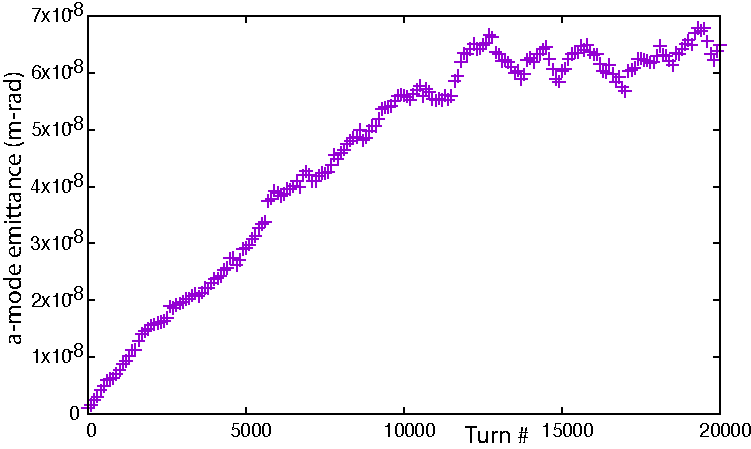
\includegraphics[width=0.8\linewidth]{figures/emit.pdf}
  \caption{The $a$-mode emittance as a function of turn number.}
  \label{f:emit}
\end{figure}

Besides particle output files, the \ltt program can generate several other types of output.
One useful type of output are the averages files. To illustrate these files, run the \ltt program with the input files
in the \vn{/lattices/10_LongTermTracking/AveragesOutput} directory. In this case, the master input file is named
\vn{averages.init}:
\begin{code}
&params
  ltt%lat_file = "simple_ring.bmad"         ! Lattice file

  ltt%averages_output_file = "#.dat"
  ltt%averages_output_every_n_turns = 100

  ltt%simulation_mode = "BEAM"
  ltt%tracking_method = "MAP"   !
  ltt%n_turns = 20000                         ! Number of turns to track
  ltt%map_order = 3

  bmad_com%spin_tracking_on = T         ! See Bmad manual for bmad_com parameters.
  bmad_com%radiation_damping_on = T
  bmad_com%radiation_fluctuations_on = T

  beam_init%n_particle = 100
  beam_init%spin = 1, 1, 0              ! See Bmad manual for beam_init_struct parameters.
  beam_init%a_emit = 1e-9
  beam_init%b_emit = 1e-12
  beam_init%sig_z = 1e-4
  beam_init%sig_pz = 1e-4
/
\end{code}
The \vn{ltt%tracking_method} is set to "\vn{MAP}" which means that tracking is done using a one-turn map.
Using a map makes tracking fast but the construction of the map at the beginning can take some time. In this case,
a very simple lattice is used to speed up the process. If radiation effects are turned on as they are here, the
radiation effects are included in the map. The map is partially inverted to make, in the limit of no radiation, the
application of the map symplectic.

The setting of \vn{ltt%averages_output_file} to "\vn{\#.dat}" means that the averages output files will be produced.
There are three averages output files which in this case will be named \vn{emit.dat}, \vn{ave.dat}, and \vn{sigma.dat}.
Every 100 turns (set by \vn{ltt%averages_output_every_n_turns}), a line is written to each file recording varias
averaged quantities like the beam sigma matrix, emittance, spin polarization, etc. 

In the init file,
the beam is specified by the \vn{beam_init} settings rather than an beam file and the beam is started with transverse
emittances that are smaller than the equilibrium ones. This is illustrated by the 
the graph in Fig.~\ref{f:emit}, which shows the approach to equilibrium of the $a$-mode emittance as
a function of turn number. 
Since the averages files are structured to be easily plotted using \vn{gnuplot}, fig.~\ref{f:emit}
was drawn with the command
\begin{code}
gnuplot> plot "emit.dat" using 1:4
\end{code}

\newpage

%------------------------------------------------------------------------------
\subsection{Exercises}

\begin{enumerate}[leftmargin=*]
%
\item {\bf Initial parameters:} 
Experiment with different initial particle parameters and plot their trajectories. 
How much can you change $pz$ without losing the particle? Track particles and plot their longitudinal phase space. 
Find stable and unstable fixed points, and invariant ellipses in longitudinal phase space.
%
\item {\bf Core Emittance:}
In the \vn{emit.dat} file there are columns for the ``50\% Core'' emittance. What is this? Hint: Consult the \ltt manual.
%
\end{enumerate}

\newpage

%------------------------------------------------------------------------------
%------------------------------------------------------------------------------
\section{Control Elements}
\label{s:control}

%----------------------------------------------------------
\subsection{Overview}

Control elements are elements that control the parameters of other elements. There are four types
of control elements: \vn{groups}, \vn{overlays}, \vn{ramper} and \vn{girders}. \vn{Groups} and
\vn{overlays} are convenient to do such things as simulate control room "knobs". For example a power
supply that powers a chain of magnets. \vn{Girder} elements
are used for simulating lattice element support structures. 
For example, a bend element followed by a quadrupole followed by a sextupole that are all
resting on a common table can be simulated with the three elements supported by a girder element. 
\vn{Ramper} elements are used for simulating machines where parameters can vary turn-by-turn. For example,
ramper elements can simulate such things as energy ramping, beta squeeze to achieve colliding beam conditions, or
third order resonance slow extraction from a ring to an extraction line.

Discussion of \vn{girder} and \vn{ramper} elements is outside the scope of this tutorial and here \vn{group} and
\vn{overlay} elements will be studied.
Note: \vn{Group}, \vn{overlay}, \vn{ramper}, and \vn{girder} elements are known as ``\vn{minor} \vn{lords}'' since they
only control a subset of an element's attributes. The other type of \vn{lord} elements, \vn{multipass} lords
and \vn{superposition} lords are called ``\vn{major lords}''. See the \bmad manual for details.

%----------------------------------------------------------
\subsection{Example Lattice}

The lattice used to illustrate control elements is named \vn{control.bmad}  which is situated in the directory \vn{/lattices/11_ControlElements/}:
\begin{code}
! Lattice File: control.bmad
beginning[beta_a] = 10
beginning[beta_b] = 10

parameter[particle] = muon
parameter[p0c] = 1e9
parameter[geometry] = open

q: quadrupole, l = 1
b: sbend, l = 1
ll: line = (q, b)
use, ll

ov1: overlay = {q[k1]: a+b^2, b[g]: 0.1*a+tan(b)}, var = {a, b}, a = 0.02
ov2: overlay = {q[k1]: 0.7, q[x_offset]: 0.1*hh}, var = {hh}, hh = 0.01
gr1: group = {b[k1]: 0.4*sqrt(z)}, var = {z}
\end{code}

Explanation:
\vspace{-5 pt}
\begin{itemize}[leftmargin=*]
%
\item
The overlay \vn{ov1} controls two parameters: 
The \vn{k1} attribute of element \vn{q} (denoted \vn{q[k1]}) and the \vn{g} attribute of element
\vn{b} (denoted \vn{b[g]}).
\item
Overlay \vn{ov1} has two variables called \vn{a} and \vn{b} that are used to control the two attributes.
\item
The formulas that overlay \vn{ov1} uses to calculate the values of the two controlled
attributes are \vn{a+b$^2$} for \vn{q[k1]} and \vn{0.1*a+tan(b)} for \vn{b[g]}.
\item 
Since overlay \vn{ov2} also controls \vn{q[k1]}, the value of \vn{q[k1]} is the sum of the
contributions of \vn{ov1} and \vn{ov2}.
\item
The given "formula" for the control of \vn{q[k1]} by \vn{ov2} is just a constant: 0.7.  This is a
shorthand notation and the actual formula used is \vn{0.7*hh}.  Note: When this shorthand notation
is used, only one control variable (in this case \vn{hh}) may be used by the overlay.
\item
The initial values for control variables may be set when defining the control element. For example,
\vn{hh} of \vn{ov2} is set to 0.2. Control variables default to a value of zero.
\end{itemize}

%----------------------------------------------------------
\subsection{Control Element Organization in the Lattice}

Start \tao with the lattice file \vn{control.bmad}. To see the elements in the lattice use the \vn{show lattice} command:
\begin{code}
Tao> show lat

      Values at End of Element:
 Index  name      key                       s       l    beta     phi ...
                                                            a       a ...
     0  BEGINNING Beginning_Ele         0.000     ---   10.00   0.000 ...
     1  Q         Quadrupole            1.000   1.000    9.83   0.101 ...
     2  B         Sbend                 2.000   1.000    9.60   0.204 ...
     3  END       Marker                2.000   0.000    9.60   0.204 ...
Lord Elements:
     4  OV1       Overlay               2.000     ---    9.60   0.204 ...
     5  OV2       Overlay               1.000     ---    9.83   0.101 ...
     6  GR1       Group                 2.000     ---    9.60   0.204 ...
 Index  name      key                       s       l    beta     phi ...
                                                            a       a ...
      Values at End of Element:
\end{code}

The list of lattice elements is divided up into two sections:
\vspace{-5 pt}
\begin{itemize}[leftmargin=*]
\item
The \vn{"tracking"} part of the lattice are the elements to be tracked through. Here the tracking
part of the lattice contains elements with index 1 through 3 (the \vn{beginning} element with index
0 is not tracked through and is present to hold Initial parameters like the Twiss parameters).
%
\item
The \vn{"lord"} section of the lattice are where the lord elements reside.  Here the lord section contains
elements with index 4 through 6.
%
\item
\vn{Group} and \vn{overlay} elements get assigned a longitudinal \vn{s}-position based upon the
\vn{s}-position of the last slave element. This does not affect any calculations and is done since it
can be useful information when using the \vn{show lat} and other \vn{show} commands (oftentimes a control
element will only control the parameters of one slave element).
\end{itemize}

\newpage

%----------------------------------------------------------
\subsection{Overlay Control}

To see how things are controlled, the \vn{show element} command may be used. Examining the lord \vn{ov1} element shows:
\begin{code}
Tao> show ele 4    ! Or: show ele ov1

 Element #                4
 Element Name: OV1
 Key: Overlay
... etc...
Slave_status: Free
Lord_status:  Overlay_Lord
Control Variables:
    1   A                                         =  2.0000000E-02
    2   B                                         =  0.0000000E+00
Slaves: [Attrib_Val = Expression_Val summed over all controlling overlays.]
   Index   Ele_Name   Attribute Attrib_Value  Expression_Val    Expression
       1   Q          K1          2.7000E-02      2.0000E-02    a+b^2
       2   B          G           2.0000E-03      2.0000E-03    0.1*a+tan(b)
... etc...
\end{code}

\begin{itemize}[leftmargin=*]
\item
All lattice elements have a \vn{slave_status} which shows what type of slave the element is and a
\vn{lord_status} which shows what type of lord the element is. \vn{overlay} elements automatically
have a \vn{lord_status} of \vn{overlay_lord}. In this case, \vn{ov1} has a \vn{slave_status} of
\vn{free} since there are no other lord elements that control parameters of \vn{ov1}. In general,
\vn{overlay} and \vn{group} lords may control parameters of other lords as well as non-lords.
\item
When an element parameter is controlled by one or more overlays, the value of that element parameter
is the sum of the values for each overlay. Thus in the above example, the contribution to \vn{q[k1]} due
to overlay \vn{ov1} is 0.02 (= $a+b^2$) as shown in the ``\vn{Expression_Val}'' column above. There is 
also a contribution of 0.007 (= $0.7 \cdot hh$) due to overlay \vn{ov2} making the value of \vn{q[k1]}
equal to 0.027 as shown in the ``\vn{Attrib_Value}'' column above. 
\end{itemize}

Examining the \vn{q} slave element shows that indeed the \vn{k1} attribute has a value of 0.027:
\begin{code}
Tao> show ele q
 Element #                1
 Element Name: Q
        ... etc...
    1   L                           =  1.0000000E+00 m
    4   K1                          =  2.7000000E-02 1/m^2
        ... etc...
Slave_status: Minor_Slave
Controller Lord(s):
   Index   Name        Attribute           Lord_Type           Expression
       4   OV1         K1                  Overlay             a+b^2
       5   OV2         K1                  Overlay             0.7*hh
       5   OV2         X_OFFSET            Overlay             0.1*hh

Lord_status:  Not_a_Lord
        ... etc...
\end{code}

The \vn{slave_status} of element \vn{q} is set to \vn{minor_slave} to show that it is controlled by
one or more minor lords. The \vn{lord_status} of \vn{q} is \vn{not_a_lord} indicating that it does
not control anything (``tracking elements'', that is elements in the tracking part of the lattice,
never control other elements).

Since the value of an attribute that is controlled by overlays depends directly on the overlay
variable values, the attribute may not be directly changed. For example, trying to change
\vn{q[k1]} directly will result in an error:
\begin{code}
Tao> set ele q k1 = 0.02
[ERROR | 2017-AUG-26 13:29:26] attribute_free:
    THE ATTRIBUTE: K1
    OF THE ELEMENT: Q
    IS NOT FREE TO VARY SINCE:
    IT IS CONTROLLED BY THE OVERLAY: OV1
\end{code}

%----------------------------------------------------------
\subsection{Group Control}

\vn{Overlay} elements use what is called ``\vn{absolute}'' control since the value of a controlled
parameter is determined directly by the settings of the overlay variables that the controlled
parameter is slaved to.  On the other hand, \vn{group} elements use what is called ``\vn{relative}''
control which is different from absolute control in two respects:
\begin{itemize}
\item
Only changes in group variable values affect controlled parameters.
\item
With group control, a controlled parameter may be varied directly.
\end{itemize}

Looking at an example will make this clear. Starting from the \vn{control.bmad} lattice, consider the effect
of changing the \vn{z} variable of the group \vn{gr1} to 0.01.
\begin{code} 
Tao> set ele gr1 z = 0.01

Tao> show ele gr1
 Element #                6
 Element Name: GR1
 Key: Group

... etc...    

Slave_status: Free
Lord_status:  Group_Lord
Control Variables:
    1   Z  =  1.0000000E-02           OLD_Z  =  1.0000000E-02
Slaves:
   Index   Ele_Name  Attribute   Attrib_Value  Expression_Val    Expression
       2   B         K1            4.0000E-02      4.0000E-02    0.4*sqrt(z)
\end{code}
For \vn{group} elements, \bmad keeps track of what is called the ``old'' value of a variable. The
name of the old value is the variable name with a ``\vn{old_}'' prefix. In this case the old value
of \vn{z} is given the name ``\vn{old_z}''. Before the \vn{set ele gr1} command was executed, the
value of \vn{z} and \vn{old_z} is zero. When the above \vn{set ele gr1} command is executed, the
value of \vn{z} becomes 0.01. \bmad detects that \vn{z} and \vn{old_z} are different and updates
\vn{b[k1]} using the following procedure: \vspace{-5 pt}
\begin{enumerate}
\item
Evaluates the formula for \vn{b[k1]} using \vn{z} and \vn{old_z} and takes the difference.
In this case the difference is \vn{0.4*sqrt(z)} - \vn{0.4*sqrt(old_z)} = 0.04
\item
Changes the value of \vn{b[k1]} by the difference (0.04).
Since the old value of \vn{b[k1]} was zero. The new value of \vn{b[k1]} is 0.04.
\item
Sets the value of \vn{old_z} equal to \vn{z} indicating that the change was made.
\end{enumerate}
A consequence of the last step in the above procedure, the \vn{show ele} command will
always show that \vn{old_z} and \vn{z} are equal.

Now consider the effect of the following commands:
\begin{code}
Tao> reinit tao
Tao> set ele gr1 z = 0.01
Tao> set ele b k1 = 0.02
Tao> set ele gr1 z = 0.04
\end{code}

The result is:

\begin{code}
Tao> show ele gr1
... etc...
Control Variables:
    1   Z  =  4.0000000E-02           OLD_Z  =  4.0000000E-02
Slaves:
   Index   Ele_Name  Attribute   Attrib_Value  Expression_Val    Expression
       2   B         K1            6.0000E-02      8.0000E-02    0.4*sqrt(z)
\end{code}
\vspace{-5 pt}
\begin{enumerate}
\item
The ``\vn{reinit tao}'' command resets \tao to its initial state.
\item
The ``\vn{set ele gr1 z = 0.01}'' command acts as explained above.
\item
The ``\vn{set ele b}'' command sets the value of \vn{b[k1]} to 0.02. This is independent of the state of element \vn{gr1}.
\item
The ``\vn{set ele gr1 z = 0.04}'' command sets the value of \vn{gr1[z]} to 0.04 which causes the
value of \vn{b[k1]} to increase by 0.04 (= 0.08 - 0.04) from 0.02 to a value of 0.06.
\end{enumerate}

\subsection{Example:}
Consider the situation where you want to control the
chromaticity (change in tune with particle energy) of a ring by varying sextupole strengths. To
change the chromaticity by 1 unit you want to change the sextupole strengths by amounts that you
compute. Here you don't care about the value of the sextupole strengths per se, you only want to vary the
sextupole strengths by a certain delta. So the sextupole ``knob'' can be simulated using a \vn{group}
controller which may look like:
\begin{code} 
xqune_1 : group ={SEX_08W:-.6415E-03*k2,...}, var = {k2}
\end{code}
Note: In this case, since the parameter to be controlled for the \vn{sex_08w} element was not specified,
the parameter is taken to be the same as the variable of the controller. \vn{k2} in this case.

Notes:
\vspace{-5 pt}
\begin{itemize}[leftmargin=*]
\item
Group and overlay elements can control other group and overlay elements.
\item
A given element parameter may only be controlled by a set of group elements or a set of overlay
elements but may not be controlled by both group and overlay elements since this would create
an ambiguous situation as to how to evaluate the parameter.
\end{itemize}

%------------------------------------------------------------------------------
\subsection{Exercises:}

\begin{enumerate}[leftmargin=*]
\item 
The function that a controller uses to control a slave attribute may be specified using an
arithmetical expression as in the above examples, or may be specified by a list of ``\vn{knot}''
points with spline interpolation used to evaluate the function in between points.  As an exercise,
setup a controller in \vn{control.bmad} that uses knot points that mimics the action of \vn{ov2} at least over some
limited interval. Hint: Look at the documentation for \vn{overlay} or \vn{group} elements in the
\vn{elements} chapter of the \bmad manual.
%
\item
\vn{Group} controllers are good for varying the longitudinal position of elements. Starting with the
file simple.bmad add a group controller that varies the \vn{s}-position of the upstream edge of
element \vn{B} while keeping the length of the entire lattice constant (hint: The lengths of both
\vn{B} and \vn{D} must change in tandem). This situation occurs frequently enough that there is a
shortcut attribute called \vn{start_edge} that can be used instead of directly varying the lengths
of elements. See the documentation on \vn{group} elements in the \vn{Elements}
chapter of the \bmad manual for more details.
%
\item
Modify the lattice file \vn{simple.bmad} to include a \vn{girder} element supporting elements \vn{B}
and \vn{Q}. Use the \vn{show ele} command to verify that indeed the girder is supporting these two
elements.
\end{enumerate}

\newpage

%------------------------------------------------------------------------------
%------------------------------------------------------------------------------
\section{Dynamic Aperture}
Dynamic aperture (DA) is measure of the stable phase space in an accelerator over a specified number of turns. Particles outside of the DA will be driven to large amplitudes where they will be lost. In the following sections, strategies for increasing a ring's DA will be shown in a sample ring.

\begin{figure}[h!]
  \centering
  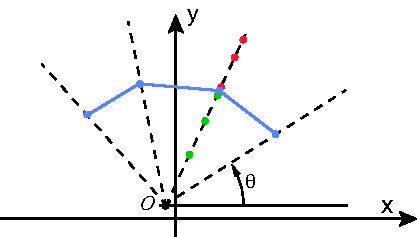
\includegraphics[width=4in]{figures/aperture-rays.pdf}
  \caption{
The calculation of a dynamic aperture curve in the $x$-$y$ plane at a given initial $p_z$ value
involves calculating aperture curve points (blue dots) along a set of ``rays'' (dashed lines). 
The line segments between
points is simply for visualization purposes and does not appear in graphs of real data. 
  }
  \label{f:da-ray}
\end{figure}

%------------------------------------------------------------------------------
\subsection{Calculating Dynamic Aperture}

The DA calculation can be done in Tao or the standalone \textit{dynamic_aperture} program. The calculation is done using the same \bmad based routines in both programs. Example files for both programs are provided. 
Points along rays are tested to determine the DA perimeter as shown in Fig.~\ref{f:da-ray}.
The rays have a common origin point ($\cal O$) which is taken to be the reference orbit. 
The calculation of an aperture curve point along a
given ray involves iteratively tracking particles with different starting $(x, y)$ position values
to find the boundary between stable (green dots) and unstable (red dots) motion.

Files for this example can be found at 
\begin{code}
/lattices/12_DynamicAperture/12.1_CalculatingDA
\end{code}
Using the init file \vn{tao_DA.init}, Tao will calculate the DA of out lattice. The DA calculation is defined in the block:
\begin{code}
&tao_dynamic_aperture
 ix_universe = 1
 ellipse_scale = 10
 pz = 0.00, 0.002, 0.004, 0.006, 0.008, 0.010
 da_param%n_angle = 5
 da_param%n_turn = 1000
 da_param%abs_accuracy = 1e-4
 da_param%min_angle = 0
 da_param%max_angle = 3.14159
 a_emit = 2E-08
 b_emit = 1E-08
/
\end{code}

\begin{figure}[tb]
  \centering
  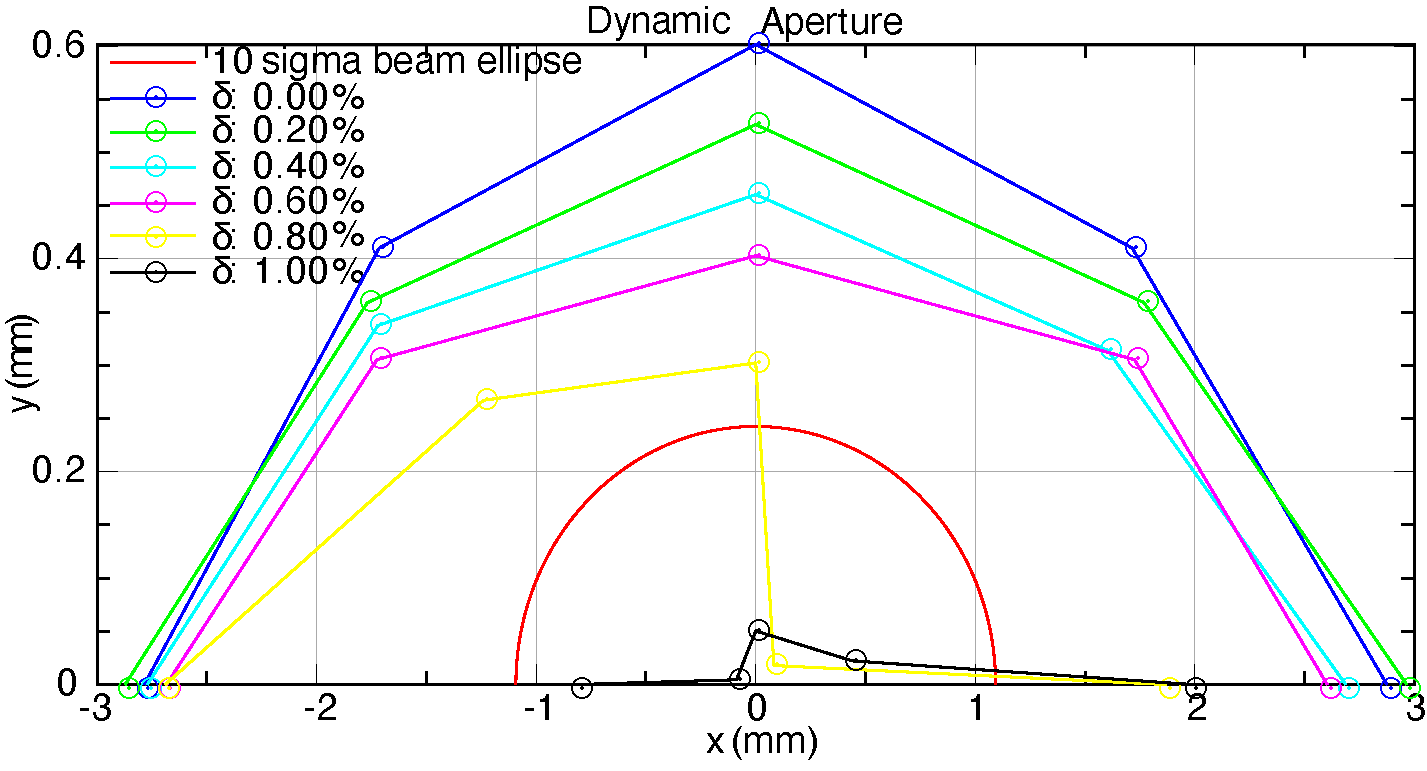
\includegraphics[width=4in]{figures/da0.pdf}
  \caption{
Dynamic aperture results.
  }
  \label{f:da0}
\end{figure}

The \vn{pz} list gives each momentum offset the aperture will be calculated for. The \vn{da_param} struct contains the parameters used for a calculation. In this case it is set up to give 5 points along rays arranged from 0 to $\pi$. Particle stability is checked over 1000 turns. Run \tao with the command
\begin{code}
tao -init tao_DA.init
\end{code}
After the calculation is finished, the results can be plotted using the command 
\begin{code}
place r11 dynamic_aperture
\end{code}
The results are shown in Fig.~\ref{f:da0}

For the standalone program, the file \vn{DA.init} is provided. The parameters are similar to those in the Tao program:
\begin{code}
&params
 dat_file = "ring_DA.dat"
 ltt%lat_file = "ring.bmad"
 ltt%rfcavity_on = T
 dpz = 0.000, 0.002, 0.004, 0.006, 0.008, 0.010
 da_param%n_angle = 5
 da_param%n_turn = 1000
 da_param%abs_accuracy = 1e-5
 da_param%min_angle = 0
 da_param%max_angle = 3.14159
/
\end{code}

The main additions are the output file and lattice file being declared. Using this file, the standalone program can be run by the command:
\begin{code}
dynamic_aperture DA.init
\end{code}
After running, the results will be in the \vn{dat_file} used. The results can the be plotted in \textit{gnuplot} using the command outputted at the end of the DA run or using the plotting software of your choice.

You can run the program using the ring lattice to check the DA. DA calculations can be slow, so it is sometimes advisable to reduce the accuracy, number of turns, or number of angles  to get faster results between optimizations, and then come back with a more accurate run to verify. These example parameters are set to take fewer than 5 minutes with the tutorial ring.

%------------------------------------------------------------------------------
\subsection{Example: Adding Sextupoles}

Files for this example can be found at: 
\begin{code}
/lattices/12_DynamicAperture/12.2_AddingSextupoles
\end{code}
A common element used for DA optimization are sextupoles. ``\vn{Harmonic}'' sextupoles, that is, sextupoles that minimize resonance driving modes, can be used to increase the transverse aperture. Sextupoles can be added to the lattice by following the steps below.

\begin{enumerate}[leftmargin=*]
%
\item Start by defining the chromatic sextupoles (sextupoles that will control the chromaticity and therefore have to be placed in dispersive regions). 
Two families per plane in each arc will be used. A typical sextupole here looks like:
\begin{code}
SF1_1: Sextupole, L = 0.584, k2 = 2
\end{code}
The sextupole strength will be optimized later. The \vn{ring.bmad} file defines a ring with sextupoles.
\item Harmonic sextupoles should also be defined for the straight sections. We will use one family in each plane
\begin{code}
SFSS: Sextupole, L = 0.584, k2 = 0.
SDSS: Sextupole, L = 0.584, k2 = -0.   
\end{code}
\item We need to make room for the sextupoles, so we will split the drift \vn{D2} into two smaller drifts
\begin{code}
D2S1: Drift, L = 0.501
D2S2: Drift, L = 0.156
\end{code}
\item The FODO cells must be altered to include the new sextupoles and drifts. In the straight sections this is simply done:
\begin{code}
! Straight section forward FoDo:
FODOSSF: line = (QFSS, D1, DB, D2S1, SDSS, D2S2, 
                 QDSS, D1, DB, D2S1, SFSS, D2S2)
\end{code}
This also must be done for the reverse line.
The arc FODOs are more  complicated as we want to families per plane. In order to do this, we will define two FODO cells. For arc 1 this will look like:
\begin{code}
! 1 o'clock arc forward 2*FoDo:
FODOAF_1: line = (QF, D1, B, D2S1, SD1_1, D2S2, 
                  QD, D1, B, D2S1, SF1_1, D2S2,
                  QF, D1, B, D2S1, SD2_1, D2S2, 
                  QD, D1, B, D2S1, SF2_1, D2S2)

\end{code}
The sample file contains similar FODO declarations for all arcs.
\item Finally the lines that define the ring must be to include the altered FODO cells
\begin{code}
SEXTANT1:  line = (4*FODOSSF, SS_TO_ARCF, 
                   10*FODOAF_1, ARC_TO_SSF_2, 4*FODOSSF_2)
SEXTANT3:  line = (4*FODOSSR_2, SS_TO_ARCR_2, 
                   10*FODOAR_3, ARC_TO_SSR, 4*FODOSSR)
SEXTANT5:  line = (4*FODOSSF, SS_TO_ARCF, 
                   10*FODOAF_5, ARC_TO_SSF, 1*FODOSSF, IPF)
SEXTANT7:  line = (IPR, 1*FODOSSR, SS_TO_ARCR, 
                   10*FODOAR_7, ARC_TO_SSR, 4*FODOSSR)
SEXTANT9:  line = (4*FODOSSF, SS_TO_ARCF, 
                   10*FODOAF_9, ARC_TO_SSF, 2*FODOSSF, 2*FODORF)
SEXTANT11: line = (2*FODORF, 2*FODOSSR, SS_TO_ARCR, 
                   10*FODOAR_11, ARC_TO_SSR, 4*FODOSSR)
\end{code}
\end{enumerate}

%------------------------------------------------------------------------------
\subsection{Example: Chromaticity Correction}

Files for this example can be found at: 
\begin{code}
/lattices/12_DynamicAperture/12.3_ChromaticityCorrection
\end{code}
The first step in chromatic correction is to use the newly placed chromatic sextupoles to correct the linear chromaticity. As there is a chromaticity associated with each plane, we have two things to correct. For optimization, sextupoles can be combined using an \vn{Overlay} element. This allows all sextupoles in the same plane to be optimized together. With one overlay for each plane, this gives two variables for the correction. This optimization can be done with the following steps:

\begin{enumerate}[leftmargin=*]
\item First the overlays must be defined
\begin{code}
OSF: overlay = {SF%_*[k2]: x}, var = {x}
OSD: overlay = {SD%_*[k2]: x}, var = {x}
\end{code}

The overlays define an attribute \vn{x} that controls the \vn{k2} attribute of every sextupole that fits a name of the form in each overlay. 
\item In the \vn{tao.init} file, a variable block can be used to control the overlays in an optimization
\begin{code}
&tao_var
    v1_var%name = 'OS'
    var(1:2)%ele_name = "OSF", "OSD"
    default_step = 1e-6
    default_attribute = 'x'
/
\end{code}
\item We must also define the data for chromaticity in the \vn{tao.init} file. Instead of correcting setting the chromaticity to zero, it is usually set to a small positive number when above transition or a small negative number when below. This is done to avoid the head-tail instability. In our case we can set it to 1 in both planes.
\begin{code}
&tao_d2_data
    d2_data%name = 'chrom'
    n_d1_data = 1
/

&tao_d1_data
    ix_d1_data = 1
    datum(1) = 'chrom.a' '' '' '' 'target' 1 100
    datum(2) = 'chrom.b' '' '' '' 'target' 1 100
/
\end{code}
\item The optimization can be done using the command \vn{run lmdif}. After the optimizer is finished, the results will be in a output file named \vn{var1.out} by default.
\item After optimizing, make a copy of the \vn{var1.out} file and rename it to something like \vn{correction.out}. Then, call the output file for the sextupole values in your lattice using \vn{call, file = correction.out}.
\item You can then rerun a DA calculation to see how this correction has altered the results.
\end{enumerate}


%------------------------------------------------------------------------------
\subsection{Advanced Dynamic Aperture Correction}

In addition to linear chromaticity, several other optimizations to improve DA are also available in Bmad. One of these is the W-function:

\begin{equation}
    W=\sqrt{A^2+B^2}
\end{equation}

where

\begin{equation}
    A=\frac{\partial\alpha}{\partial p_z}-\frac{\alpha}{\beta}\frac{\partial\beta}{\partial p_z}, \;\;\;\;\;\;\;    B=\frac{1}{\beta}\frac{\partial\beta}{\partial p_z}
\end{equation}

This is a chromatic function that is the amplitude of the linear energy dependent $\beta$-beat. similar to the linear chromaticity, this can be corrected with the use of sextupoles. This correction is more complex than before as the phase advance between sextupoles and the quadrupoles creating the W-function is important. Since $\beta$-beating goes as twice the betatron phase advance, sextupoles that are 90\degree apart will work against each other. The solution is to split the sextupoles in each arc into two families per plane. This way we can correct the chromaticity while making sure the sextupoles do not entirely cancel each other for the W-function correction. 

\subsubsection{Example}

Files for this example can be found at: \\ \vn{/lattices/12_DynamicAperture/12.4_AdvancedDA}

The sextupole families can again be set up using an overlay, although this time we will center the sextupole strengths around the value for chromaticity correction. This will ensure each arc corrects an equal amount of the total chromaticity. 

\begin{enumerate}[leftmargin=*]
    \item We will begin by altering the overlays. Assume the sextupole setting you found in the last example are SX and SY, then an overlay for sextupoles centered at these values will be
    \begin{code}
    OF_1: overlay = {SF1_1[k2]:  SX + x, SF2_1[k2]:  SX - x}, var = {x}
    OD_1: overlay = {SD1_1[k2]:  SY + x, SD2_1[k2]:  SY - x}, var = {x}
    \end{code}
    This must be done for all arcs.
    \item With these overlays, the W-function can be optimized, however, without proper phasing between arcs, sextupoles may not be efficient in the correction. In order to fix phases between sextupoles for the optimization, it is often useful to use a phase trombone. Phase trombones are artificial elements that are used to set a phase advance without altering optics.
    We will need three phase trombones, two surrounding the IP and one to fix the tune. We will fix the tune in the 2 o'clock tune cell.
    \begin{code}
    TR_F: match, dphi_a = 0, dphi_b = 0, matrix = phase_trombone
    TR_R: match, dphi_a = 0, dphi_b = 0, matrix = phase_trombone
    TR_M: match, dphi_a = 0, dphi_b = 0, matrix = phase_trombone
    \end{code}
    \item In order to make sure the tune remains fixed, we can use an overlay to control the trombones
    \begin{code}
    TROMBONES: overlay = {TR_F[dphi_a]: x1, 
        TR_R[dphi_a]: x2, TR_2[dphi_a]: -x1-x2,
        TR_F[dphi_b]: y1, TR_R[dphi_b]: y2, TR_2[dphi_b]: -y1-y2},
           var = {x1, x2, y1, y2}

    \end{code}
    \item W-function optimization is often done by setting it to zero in specific location in the ring. We will set it to zero at the IP and at the end of arc 7. We will add a marker for the use in the optimization
    \begin{code}
    END_7: marker
    \end{code}
    \item The trombones and marker can now be placed in the ring
    \begin{code}
    SEXTANT1:  line = (TR_M, 4*FODOSSF, SS_TO_ARCF, 
        10*FODOAF_1, ARC_TO_SSF_2, 4*FODOSSF_2)
    SEXTANT3:  line = (4*FODOSSR_2, SS_TO_ARCR_2, 
        10*FODOAR_3, ARC_TO_SSR, 4*FODOSSR)
    SEXTANT5:  line = (4*FODOSSF, SS_TO_ARCF, 
        10*FODOAF_5, ARC_TO_SSF, 1*FODOSSF, TR_F, IPF)
    SEXTANT7:  line = (IPR, TR_R, 1*FODOSSR, SS_TO_ARCR,
        10*FODOAR_7, END_7 ,ARC_TO_SSR, 4*FODOSSR)
    SEXTANT9:  line = (4*FODOSSF, SS_TO_ARCF, 
        10*FODOAF_9, ARC_TO_SSF, 2*FODOSSF, 2*FODORF)
    SEXTANT11: line = (2*FODORF, 2*FODOSSR, SS_TO_ARCR, 
        10*FODOAR_11, ARC_TO_SSR, 4*FODOSSR)

    \end{code}
    \item We must now set up the init file. Define the W-function to be zero at the \vn{IP6} and \vn{END_7} markers
    \begin{code}
    &tao_d2_data
        d2_data%name = 'w'
        n_d1_data = 1
    /
    &tao_d1_data
        ix_d1_data = 1
        datum(1) = 'chrom.w.a' '' '' 'END_7' 'target' 0 100
        datum(2) = 'chrom.w.b' '' '' 'END_7' 'target' 0 100
        datum(3) = 'chrom.w.a' '' '' 'IP6##1'   'target' 0 100
        datum(4) = 'chrom.w.b' '' '' 'IP6##1'   'target' 0 100
    /
    \end{code}
    \item The variables can be set up to control the sextupoles in arcs 5 and 7 and the phase trombones
    \begin{code}
 &tao_var
     v1_var%name = 'sextupoles'
     var(1:4)%ele_name = "OF_5", "OD_5", "OF_7", "OD_7"
     default_step = 1e-6
     default_attribute = 'x'
/


&tao_var
    v1_var%name = 'phases'
    var(1:4)%ele_name="TROMBONES", "TROMBONES", "TROMBONES", "TROMBONES"
    default_step = 1e-6
    var(1:4)%attribute = 'x1', 'x2', 'y1', 'y2'
/

    \end{code}  
    \item Run the optimizer in Tao to find the correct sextupole and phase trombone settings.
    \item Make a copy of the \vn{var1.out} file and call it in your lattice to use the updated values.
\end{enumerate}

After these steps, you should have a W-function like in Figure~\ref{f:W-function}.


\begin{figure}[tb]
  \centering
  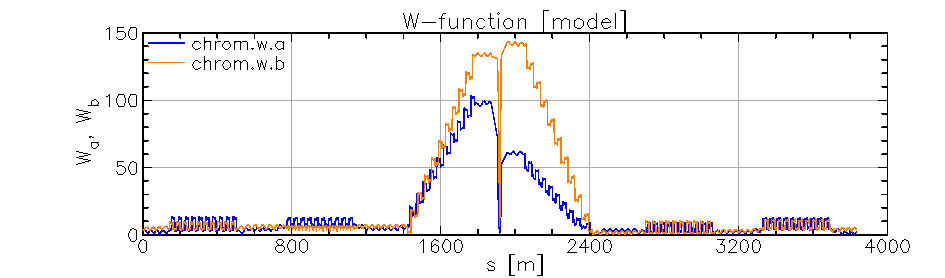
\includegraphics[width=\textwidth]{figures/W_correction.png}
  \caption{The W-function receives a large contribution form the IP which is corrected over one arc.}
  \label{f:W-function}
\end{figure}


%Dynamic aperture optimization strategies can vary between rings, and only a few of those available in Bmad were shown here. In addition to what was shown in this chapter, the following features are also available in Bmad:

%\begin{enumerate}
%    \item {W-function}
%    \item {Linear and higher order chromaticity}
%    \item {Phase trombones}
%    \item {Second order dispersion}
%    \item {Tune maps}
%    \item {Frequency maps}
%    \item {Calculation of resonance driving terms}
%    \item {Coupling matrix}
%    \item {DA calculation with ramping elements}
%    \item {DA calculation with beam-beam}
%\end{enumerate}

%------------------------------------------------------------------------------
\subsection{Exercises}

\begin{enumerate}[leftmargin=*]
    \item {\bf IP and 2 o'clock phase trombones:} This can be split into three parts, the phase on both sides of the IP and the phase in the 2 o'clock phase trombone. These parts can be inserted separately into the init file
    \begin{enumerate}
        \item The 2 o'clock phase trombone is the easiest to add the init file, simply copy the data and variables from the previous use of the tune cell.
        \item The upstream phase trombone can be implemented by fixing  $\alpha_{x,y}$ and $\beta_{x,y}$ at the IP. Add a marker at the beginning of arc 5 named \vn{END_5}. Set a datum for \vn{phase_frac.a} and \vn{phase_frac.b} from the marker to the IP. Set the target to get the correct phase. For variables, use the upstream IR quads and the last three quads in the matching section from the dispersion suppressor.
        \item The downstream phase can be matched using the same process as the upstream side. Variables can be chosen to be the downstream IR quads and last three quads in the matching section to the dispersion suppressor. We again must fix $\alpha_{x,y}$ and $\beta_{x,y}$, but this time we will fix it at the marker \vn{END_7}. The phase condition is now set from the IP to \vn{END_7}.
    \end{enumerate}
    After setting up the data and variables, you can run the optimizer. If the lattice may become unstable during the optimization, if this happens, try using the \vn{cut} command (toggles lattice geometry between open and close). Notice that the W-function correction is slightly disrupted by this change. This sometimes requires an iterative process.
\end{enumerate}
\newpage

%------------------------------------------------------------------------------
%------------------------------------------------------------------------------
\section{Model, Design and Base Lattices in Tao}
\label{s:three.lat}

When \tao runs, \tao creates three lattices
(Technically, \tao instantiates three lattices per \vn{universe}. See the discussion on universes in the \tao manual.):
\begin{description}
\item[Design Lattice] \Newline
The \vn{design} lattice corresponds to the lattice read in from the lattice
description file(s). Parameters in this lattice are never varied.
\item[Model Lattice] \Newline
Initially, when \tao is started, The \vn{model} lattice is the same as the \vn{design}
lattice. Parameters in the \vn{model} lattice are allowed to vary. That is, all commands to vary
lattice parameters vary parameters of the \vn{model} lattice.
\item[Base Lattice] \Newline
The \vn{base} lattice is a reference lattice used so that changes in the \vn{Model} lattice may be
easily viewed. The \vn{Design} lattice can also be used as a reference lattice but since the
parameters of the \vn{design} lattice are fixed, this is not always desirable. The parameters of the
\vn{base} lattice are set by setting the parameters of the \vn{base} lattice equal to the present
state of the \vn{model} lattice.
\end{description}

\begin{figure}[tb]
  \centering
  \begin{subfigure}[t]{0.48\textwidth}
    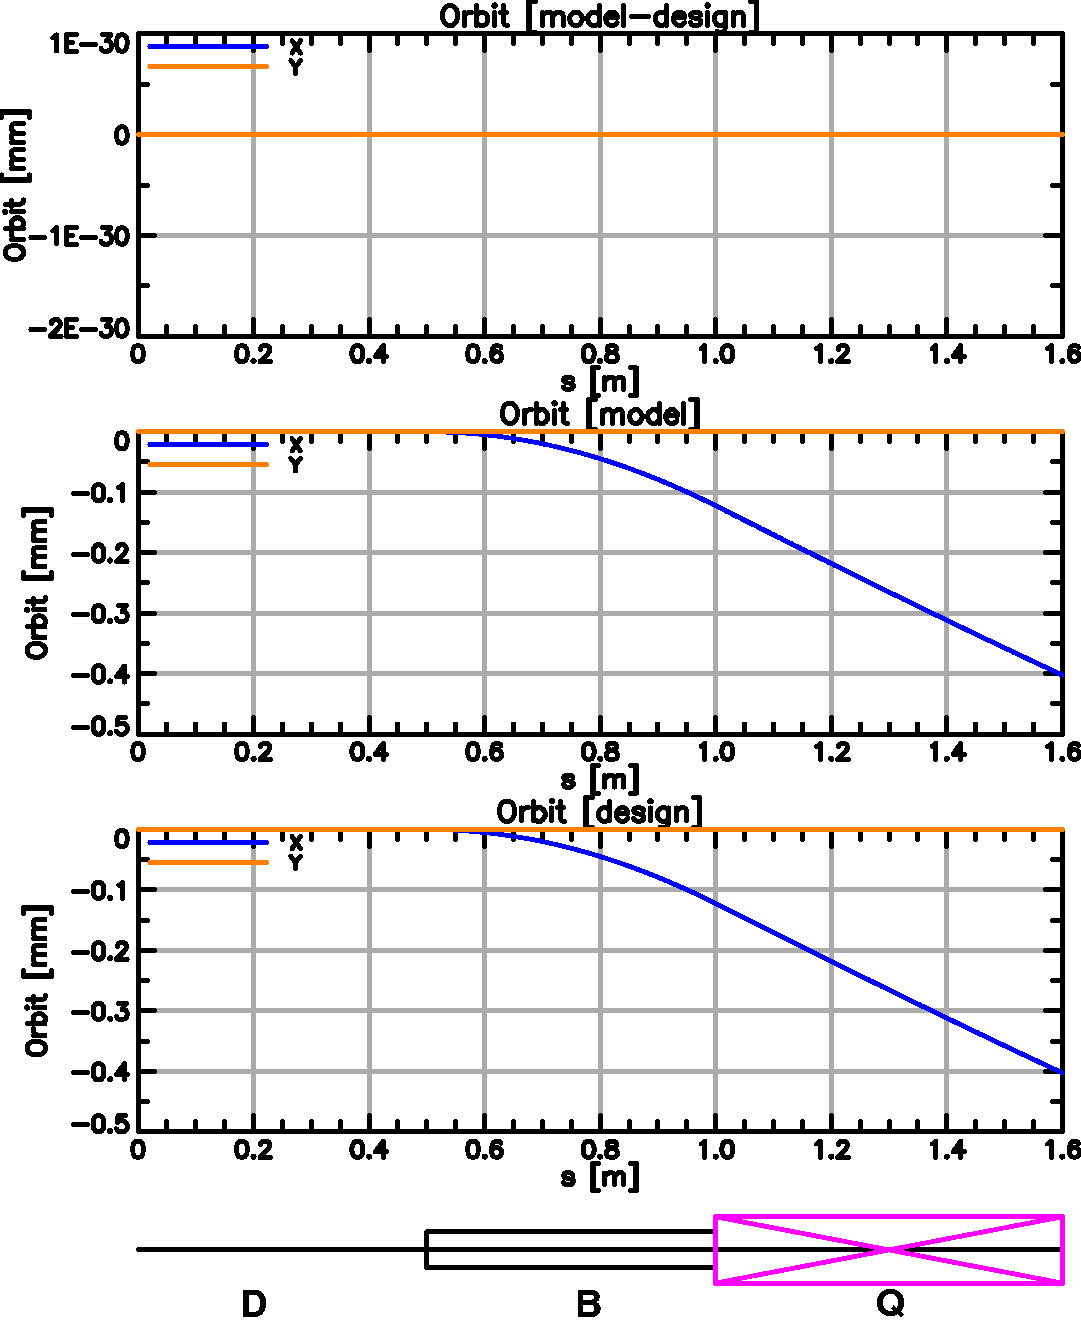
\includegraphics[width=\textwidth]{figures/model-equal-design.pdf}
    \caption{Initially, the \vn{model} lattice and the \vn{design} lattices are the same.}
    \label{f:model.eq.design}
  \end{subfigure}
  \hfil
  \begin{subfigure}[t]{0.48\textwidth}
    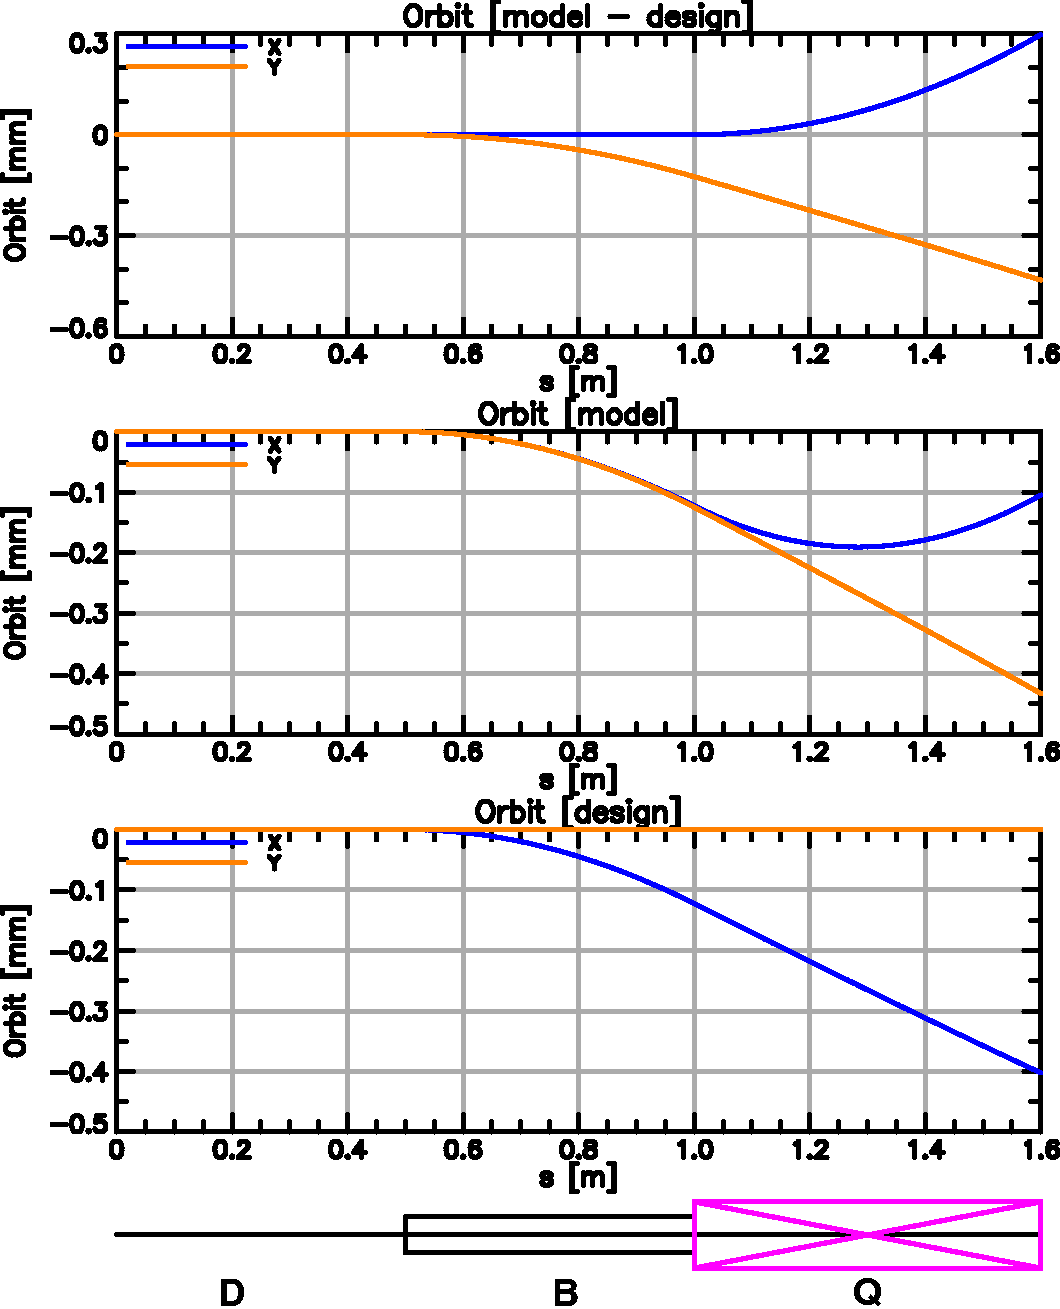
\includegraphics[width=\textwidth]{figures/changed-model.pdf}
    \caption{The \vn{set} and \vn{change} commands will modify \vn{model} lattice parameters.}
    \label{f:changed.model}
  \end{subfigure}
  \caption{}
\end{figure}

%----------------------------------------------------------
\subsection{Changing Model Parameters}
\label{s:change}

To see the difference between the \vn{model} and \vn{design} lattices, start \tao with the lattice file \vn{lattices/13_LatticeTypes/simple.bmad}.

Now issue the following commands:
\begin{code}
Tao> place r23 orbit
Tao> place r13 orbit
Tao> set plot r33 component = design          ! Bottom plot
Tao> set plot r13 component = model - design  ! Plot difference orbit
Tao> scale
\end{code}
The ``\vn{set plot <plot_name> component = ...}'' command sets where the data to be plotted
comes from.  The result is shown in Figure~\ref{f:model.eq.design}. The bottom plot shows the
\vn{design} lattice orbit, the middle plot shows the \vn{model} lattice orbit and the top plot shows
the difference in orbits between \vn{model} and \vn{design}. Since the two lattices are the same
when \tao is started, the difference orbit is zero.

Now change the \vn{model} lattice using the following commands:
\begin{code}
Tao> change element b vkick  -0.0005   ! Changes by a given delta
Tao> set element q hkick = 0.001       ! Another way of changing a parameter.
Tao> scale
\end{code}
The \vn{change} command changes real numbers by a given delta. The \vn{set} command sets a 
parameter to a specific value. Unlike the \vn{change} command, 
the \vn{set} command can also be used with integer, string and logical
parameters.  The result is shown in Figure~\ref{f:changed.model}. Since now
the \vn{model} lattice is not the same as the \vn{design} lattice, the difference orbit is non-zero.

\begin{figure}[tb]
  \centering
  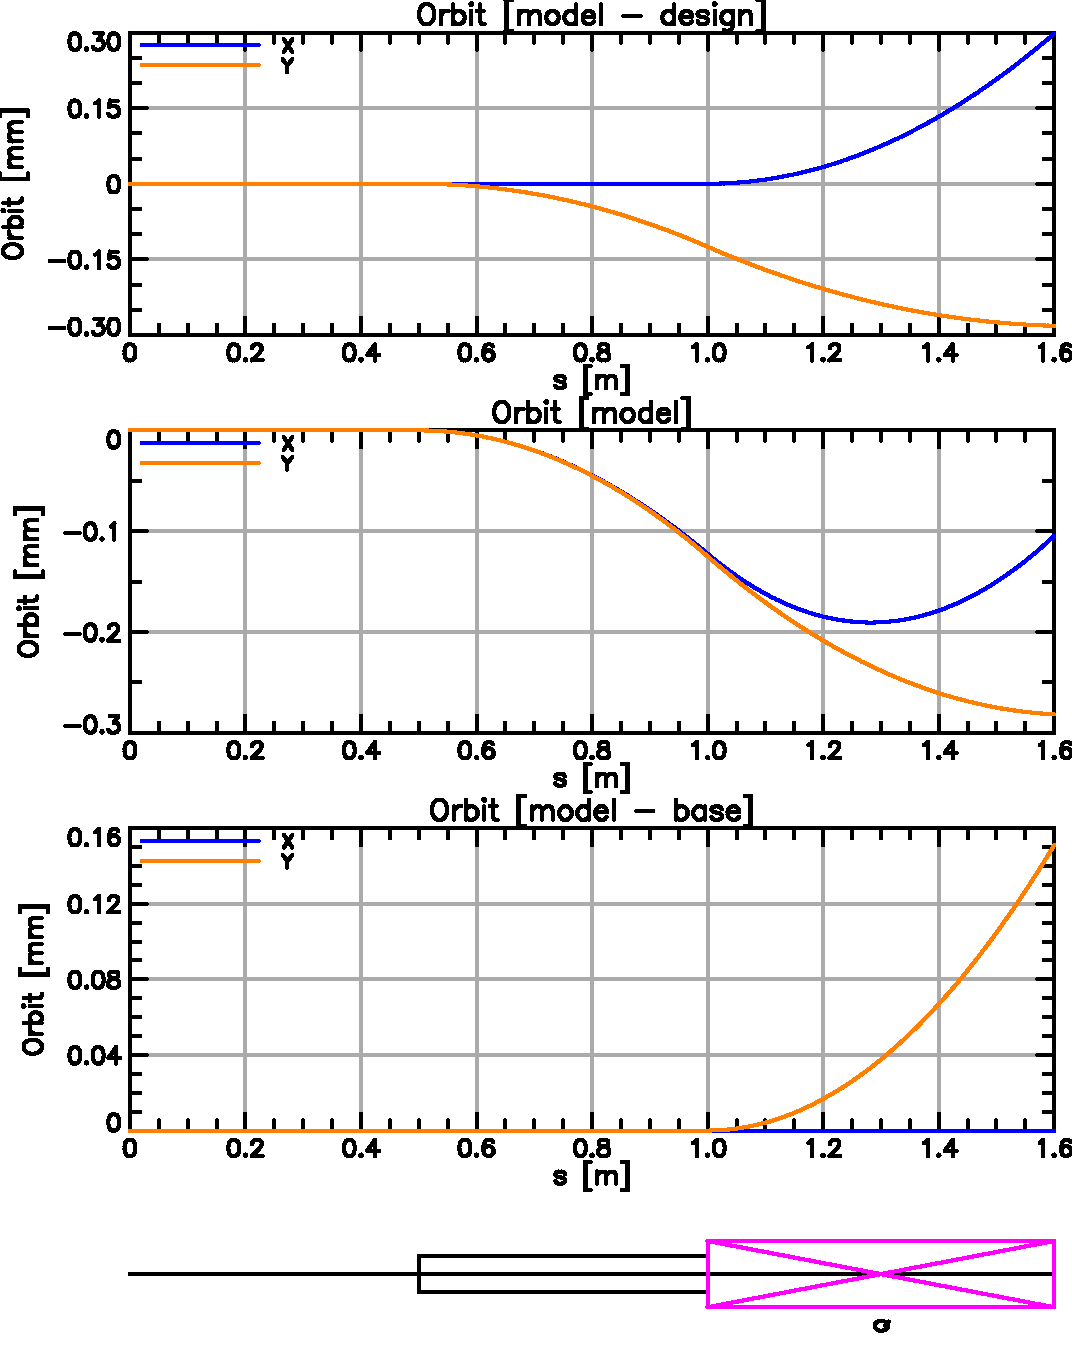
\includegraphics[width=0.6\textwidth]{figures/with-base.pdf}
  \caption{The \vn{base} lattice is used to view changes when the reference lattice configuration
does not correspond to the \vn{design} lattice.}
  \label{f:base}
\end{figure}

%----------------------------------------------------------
\subsection{Using the Base Lattice}

The \vn{base} lattice is used to view changes when the desired reference lattice does not
correspond to the \vn{design} lattice.

Continuing from the previous section, issue the following commands:
\begin{code}
Tao> set lattice base = model  ! Set the Base lattice = Model lattice.
Tao> set plot r33 component = model - base
Tao> set ele q vkick = 5e-4
Tao> scale
\end{code} 
The \vn{set lattice} command sets the \vn{base} lattice equal to the \vn{model}
lattice. The third command varies the \vn{model} lattice.  The result is shown in
Figure~\ref{f:base}. The bottom plot of the orbit difference between \vn{model} and
\vn{base} is not the same as the orbit difference between \vn{model} and \vn{design}.

\vspace{1in}

%----------------- 
\subsection{Exercises}

\begin{enumerate}[leftmargin=*]
%
\item {\bf Orbit plots:} Modify the middle graph in Fig.~\ref{f:base} so that the vertical orbit curve becomes the horizontal orbit of the \vn{design} lattice.
%
\item {\bf Alias command:} To save on typing, alias commands may be defined. Define an alias command called \vn{setit} so that typing ``\vn{setit 1e-6}'' is equivalent to ``\vn{set ele q vkick = 1e-6}''. Hint: Look in the manual or type ``\vn{help alias}'' to get more information on setting and using alias commands.
Note: Do not confuse \tao alias commands with the alias string component of a lattice element.
%
\item {\bf Adjust the tune using \vn{set tune}:} The tune of the lattice can also be set by using the \vn{set tune} command in \tao, which scales together all focusing quadrupoles and all defocusing quadrupoles to set the horizontal and vertical tunes. Using a lattice with the ring you have constrcted, use \vn{set tune -mask *,~QF,~QD 0.08 0.14} to set the tune of the ring. Plot the difference between the model and design lattices to see how much ``beta-beating'' there is around the ring.
%
\end{enumerate}

\newpage

%------------------------------------------------------------------------------
%------------------------------------------------------------------------------
\section{Orbit Correction}
\label{s:orbit}

While operating accelerators, the beam's orbit is measured with Beam Position Monitors (BPMs). The accelerator is designed with ideal BPM readings in mind; often these are 0. And after extended operational experience, operators often learn good readings for all BPMs, often referred to as golden orbits. It then becomes important to change the beam's trajectory to obtain these desired BPM readings.

%------------------------------------------------------------------------------
\subsection{Example: Adding Corrector Coils and BPMs}

\begin{figure}[!h]
  \centering
  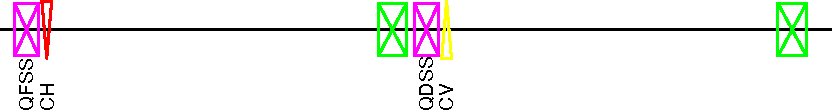
\includegraphics[width=0.9\linewidth]{figures/correctors.pdf}
  \caption{FODO cell with corrector coils.}
  \label{f:corrector}
\end{figure}

\begin{enumerate}[leftmargin=*]
\item Let's start with the \vn{ring0.bmad} lattice. We will place corrector coils in the middle of D1 drifts 6.4 cm away from quadrupoles. This is downstream from the quadrupoles in the forward arcs and upstream in the reverse arcs. Define horizontal and vertical corrector coils and appropriate drift spaces as follows:
\begin{code}
! (1): Define horizontal/vertical corrector coils and 
        split D1 into D1C1 and D1C2 to fit coils
D1C1: Drift, L = 0.064
D1C2: Drift, L = 0.345 !0.609 - 0.064 - 0.2
CH: hkicker, L = 0.2
CV: vkicker, L = 0.2
\end{code}
\item Add corrector coils near quadrupoles. We will add horizontal kickers near focusing quadrupoles and vertical kickers near defocusing quadrupoles. In both forward and reverse geometry, we will add correctors in the D1 drift, which means the correctors are after quadrupoles in the forward geometry and before quadrupoles in the reverse geometry. 

Because we have used D1 drifts repeatedly throughout the ring, adding correctors manually is a tedious task. The easiest approach is to use regular expressions in Find and Replace. The recipe is the following: 
\begin{code}
1. In the forward arcs for drifts after focusing quadrupoles:
    Replace (QF[^,\n]*,[^,\n]*)D1 with \1D1C1, CH, D1C2 for 
2. In the forward arcs for drifts after defocusing quadrupoles:
    Replace (QD[^,\n]*,[^,\n]*)D1 with \1D1C1, CV, D1C2
3. In the reverse arcs for drifts before focusing quadrupoles:
    Replace (D1)([^,\n]*,[^,\n]*QF), with D1C2, CH, D1C1\2 
4. In the reverse arcs for drifts before defocusing quadrupoles:
    Replace (D1)([^,\n]*,[^,\n]*QD), with D1C2, CV, D1C1\2
5. In the reverse arcs for drifts at the end of a cell:
    Replace D1) with D1C2, CH, D1C1) 
\end{code}
In some text editors, you may need to use \$1 and \$2 instead of \textbackslash 1 and \textbackslash 2.
\item Define and add BPMs after dipoles (\vn{B}, \vn{HB}, and \vn{DB} in the straight section). Here we use a 0-length marker to represent the BPMs.
\begin{code}
! (3) Define and add BPMs
BPM: marker
\end{code}
Then insert the BPMs after dipoles by searching and replacing \vn{B,} with \vn{B, BPM,} (including the commas) and repeat for \vn{HB} and \vn{DB}.
\end{enumerate}

%------------------------------------------------------------------------------
\subsection{Example: Radiation-induced Sawtooth Orbit Correction}
\label{s:sawtooth}

\begin{figure}[!h]
  \centering
  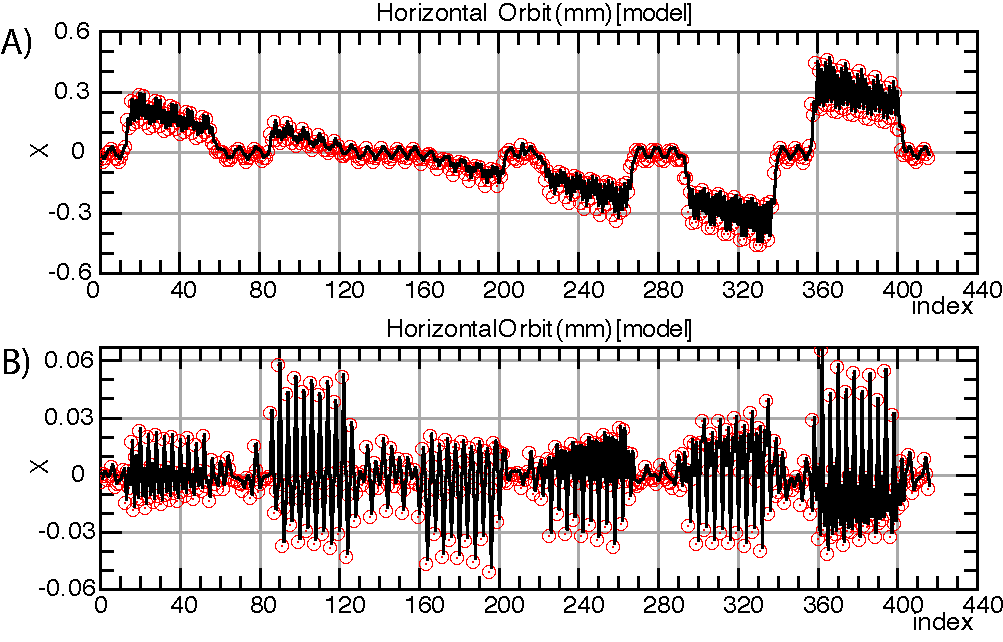
\includegraphics[width=0.9\linewidth]{figures/sawtooth.pdf}
  \caption{A) The sawtooth orbit due to synchrotron radiation. B) The orbit after correction using kickers and BPMs.}
  \label{f:sawtooth}
\end{figure}

\begin{enumerate}[leftmargin=*]
\item Turn on radiation damping with
\begin{code}
bmad_com[radiation_damping_on] = T 
\end{code}
in the lattice file, or equivalently run
\begin{code}
set bmad_com radiation_damping_on = T
\end{code}
in \tao. It turns on the deterministic average synchrotron radiation energy loss in the ring. This energy loss leads to the particle energy variation along the ring. It also causes the horizontal closed orbit to have a sawtooth shape. You should see this sawtooth orbit in \tao. Let's explore two methods to correct the sawtooth orbit.
\item The \vn{taper} command adjusts magnet strengths to eliminate the transverse orbital and Twiss changes due to the radiation damping induced sawtooth effect. The \vn{taper} scales magnet strengths based on local closed orbit momentum deviation and identical elements are changed independently. Tapering is not applied to strengths controlled by an \vn{overlay} element.

Now run \vn{taper} in \tao and check the resulting orbit.
\item Alternatively, we can use kickers to fix the sawtooth orbit. Let's define the orbit readings as data and kicker strengths as variables in \vn{tao.init}. 
\begin{code}
&tao_d2_data
  	d2_data%name = 'orbit'
  	n_d1_data = 2
  	default_merit_type = 'target'
  	default_meas = 0
  	default_weight = 1
/

&tao_d1_data
	ix_d1_data = 1
	d1_data%name = 'x'
	search_for_lat_eles = 'BPM*'
/

&tao_d1_data
	ix_d1_data = 2
	d1_data%name = 'y'
	search_for_lat_eles = 'BPM*'
/

&tao_var
	v1_var%name = 'hkicker'
	search_for_lat_eles = 'hkicker::*'
	default_step = 1e-6
	default_attribute = 'kick'
/

&tao_var
	v1_var%name = 'vkicker'
	search_for_lat_eles = 'vkicker::*'
	default_step = 1e-6
	default_attribute = 'kick'
/
\end{code}
\item Right now all the kickers and BPMs are assumed to be the same, but we want to address them individually. \tao has the option to add a unique suffix after duplicate elements. Simply add to your \vn{tao.init}:
\begin{code}
&tao_design_lattice
	unique_name_suffix = "hkicker::_? vkicker::_? marker::_?"
/
\end{code}
\item While \tao has a native template for orbit plots, here we provide two custom templates to plot orbit data from BPMs. You can add them to your \vn{tao.init} and show them by running \vn{place r13 bpm_orbit_x} and \vn{place r23 bpm_orbit_y}.
\begin{code}
&tao_template_plot
  plot%name = 'bpm_orbit_x'
  default_graph%x%major_div_nominal = 10
  default_graph%x%label = ' '
  plot%x_axis_type = 'index'
  plot%n_graph = 1
/

&tao_template_graph
  graph%name = 'x'
  graph_index = 1
  graph%box = 1, 1, 1, 1
  graph%title = 'Horizontal Orbit (mm)'
  graph%y%label = 'X'
  graph%y%major_div = 4
  curve(1)%data_source = 'data'
  curve(1)%data_type   = 'orbit.x'
  curve(1)%y_axis_scale_factor = 1000
  curve(1)%symbol%color = "red"
/

&tao_template_plot
  plot%name = 'bpm_orbit_y'
  default_graph%x%major_div_nominal = 10
  default_graph%x%label = ' '
  plot%x_axis_type = 'index'
  plot%n_graph = 1
/

&tao_template_graph
  graph%name = 'y'
  graph_index = 1
  graph%box = 1, 1, 1, 1
  graph%title = 'Vertical Orbit (mm)'
  graph%y%label = 'Y'
  graph%y%major_div = 4
  curve(1)%data_source = 'data'
  curve(1)%data_type   = 'orbit.y'
  curve(1)%y_axis_scale_factor = 1000
/
\end{code}
\item Before we run the optimization, we can choose which variables to change and which data to optimize with \vn{run} and \vn{veto} commands. For example, the sawtooth orbit is entirely in the x-direction, so we can ignore vkickers and orbit.y for this orbit correction with:
\begin{code}
veto var vkicker
veto data orbit.y
\end{code}
Run the optimizer and check if the orbit is fixed. Write the lattice with optimized kicker strengths into a new file \vn{ring.bmad}.
\end{enumerate}

%----------------------------------------------------------
\subsection{Element Misalignments}
\label{s:ele.mis}

\begin{figure}[tb]
  \centering
  \begin{subfigure}[t]{0.62\textwidth}
    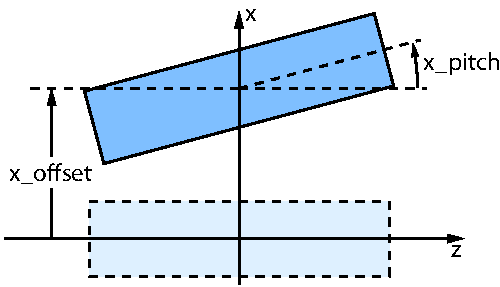
\includegraphics[width=\textwidth]{figures/pitch.pdf}
    \caption{Effect of x_offset and x_pitch on a straight line element}
    \label{f:pitch}
  \end{subfigure}
  \hfil
  \begin{subfigure}[t]{0.33\textwidth}
    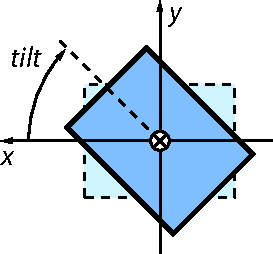
\includegraphics[width=\textwidth]{figures/tilt.pdf}
    \caption{Effect of a tilt on a straight line element.}
    \label{f:tilt}
  \end{subfigure}
  \caption{}
\end{figure}

Once the \vn{reference} coordinate system is established, the position of any physical element
can be shifted (``misaligned''). [Note: \vn{Patch} and \vn{floor_shift} elements cannot be misaligned.]
For straight elements, the element attributes that determine any misalignment are:
\begin{description}
\item[x_offset, y_offset, z_offset] \Newline
The \vn{x_offset}, \vn{y_offset}, and \vn{z_offset} attributes offset the element in the \vn{x}, \vn{y},
and \vn{z} directions respectively. See Figure~\ref{f:pitch}.
%
\item[x_pitch, y_pitch] \Newline
The \vn{x_pitch} and \vn{y_pitch} attributes rotate the element. A \vn{x_pitch} of $\pi/2$ would rotate the
element around the +\vn{y}-axis so that the body +\vn{z}-axis is aligned with the local
+\vn{x}-axis. Similarly, a \vn{y_pitch} of $\pi/2$ would rotate the element around the -\vn{x}-axis so
that the body +\vn{z}-axis is aligned with the local +\vn{y}-axis. See Figure~\ref{f:pitch}.
%
\item[tilt] \Newline
A \vn{tilt} rotates the element around the +\vn{z}-axis as shown in Figure~\ref{f:tilt}
\end{description}

Note: The above only applies to straight elements. Patch like elements are explained below. For a
discussion of misalignments for bend type elements see the \bmad manual.

\subsubsection{Example:}
\begin{code}
! Lattice File: misalign.bmad
beginning[beta_a] = 10.   ! m  a-mode beta function
beginning[beta_b] = 10.   ! m  b-mode beta function
beginning[e_tot] = 10e6   ! eV
parameter[geometry] = open  ! or closed
q: quadrupole, L = 1, x_offset = 0.1, x_pitch = 0.04
lat: line = (q)   ! List of lattice elements
use, lat          ! Line used to construct the lattice
\end{code}

Start \tao with the lattice file \vn{misalign.bmad}. The
misalignment can be viewed using the \vn{-floor} option with the \vn{show element } command:
\begin{code} 
Tao> show ele q -floor

 Element #                1
 Element Name: Q
... etc...

 Attribute values [Only non-zero/non-default values shown]:
    1  L               =  1.0000E+00 m
   13  SPIN_FRINGE_ON  =  T (1)
   31  L_HARD_EDGE     =  1.0000E+00 m
   34  X_PITCH         =  4.0000E-02       55  X_PITCH_TOT   =  4.0000E-02
   36  X_OFFSET        =  1.0000E-01 m     57  X_OFFSET_TOT  =  1.0000E-01 m
... etc...

Global Floor Coords at End of Element:
                X        Y        Z    Theta  
Reference  0.00000  0.00000  1.00000  0.00000 ... ! Without misalignments
Actual     0.11999  0.00000  0.99960  0.04000 ... ! With misalignments
... etc...
\end{code}

In the ``\vn{Global Floor Coords}'' section, the \vn{Reference} row shows the nominal position of
the \vn{exit} end of the element without misalignments. [Due to space constraints the \vn{phi} and
\vn{psi} columns are not shown. They are zero in this case.] The \vn{Actual} row shows the position
of the physical element at the \vn{exit} end.

Associated with each misalignment attribute there is a corresponding attribute with a ``\vn{_tot}''
suffix. The difference is that an attribute like \vn{x_offset} is the misalignment with respect to
any \vn{girder} (\sref{s:girder}) that may be supporting it while the corresponding
\vn{x_offset_tot} is the total misalignment of the lattice element with respect to the element's
nominal position. Another difference is that misalignments attributes are set by the user while the
corresponding \vn{_tot} attributes are calculated by \bmad. If there is no \vn{girder} support, the
\vn{_tot} attributes will be the same as the misalignment attributes as it is in this case so
\vn{x_pitch} is equal to \vn{x_pitch_tot}, etc.

%------------------------------------------------------------------------------
\subsection{Example: Orbit Correction with Quadrupole Misalignments}
\begin{enumerate}[leftmargin=*]
\item Let's start from \vn{ring.bmad} that we created in chapter~\sref{s:sawtooth}. Add random offsets to all quadrupoles in the lattice. We can first assume that x-offsets of quadrupoles follow a Gaussian distribution of $\sigma=10\unit{\mu m}$ with a $3\sigma$ cutoff. You can do this with \tao command "\vn{set ele quadrupole::* x_offset = 1e-5*ran_gauss(3)}". The \vn{ran_gauss(sig_cut)} command returns an array of Gaussian distributed random variables with unit RMS truncated at sig\_cut.

\item Correct the orbit using the same optimization process. You can reuse the \vn{tao.init} we wrote previously.

\item If the misalignment amplitude is large, it is likely that the orbit becomes unstable and the optimizer will have a hard time finding a solution. \vn{unstable.lattice} datum is used to handle these situations, which will be zero if the particle lives and positive if there is particle loss. 
\begin{code}
&tao_d2_data
  	d2_data%name = 'unstable'
  	n_d1_data = 1
/

&tao_d1_data
	ix_d1_data = 1
	d1_data%name = 'lat'
	datum(1) = "unstable.lattice" "" "" "" "target" 0 100
/
\end{code}

\item With the addition of \vn{unstable.lattice} datum, run the optimization to correct the orbit
\end{enumerate}


\subsection{Exercise}
Use 4 horizontal/vertical kickers around the IP (CH/V_104 to CH/V_107) to make the orbit exactly 0 at the IP without affecting the rest of the ring.

\newpage

%------------------------------------------------------------------------------
%------------------------------------------------------------------------------
%\section{Tracking with Ramping and Spin Tracking}

%------------------------------------------------------------------------------
%\subsection{Tracking with Ramping}
%The ESR will not be used to accelerate, however to show what ramping in Bmad might look like we include this section.

%------------------------------------------------------------------------------
%\subsection{Adding Siberian Snakes}
%Taylor element overview



%------------------------------------------------------------------------------
%\subsection{Invariant Spin Field Calculations}
%\sodom $\rightarrow$ \ltt

%\newpage

%------------------------------------------------------------------------------
%------------------------------------------------------------------------------
\appendix

%------------------------------------------------------------------------------
%------------------------------------------------------------------------------
\section{Python/PyTao Interface}

PyTao is a Python wrapper on top of Tao that allows users to access the Tao library via \vn{ctypes} and \vn{pexpect}. More information can be found at \url{https://bmad-sim.github.io/pytao/}.

%------------------------------------------------------------------------------
\subsection{Installation}

The Bmad Distribution must be installed before installing PyTao. If Bmad is installed via a release tarball, the Bmad Distribution must be compiled with the \vn{ACC_ENABLE_SHARED="Y"} flag set in the \vn{bmad_dist/util/dist_prefs} file. 

PyTao can be installed in three different ways:

1) Using setuptools
\begin{code}
python setup.py install
\end{code}

2) Using pip
\begin{code}
# From PyPI distribution
pip install pytao

# or from the source folder
pip install .

\end{code}

3) Using conda
\begin{code}
conda install -c conda-forge pytao
\end{code}

%------------------------------------------------------------------------------
\subsection{Basic Examples}

\subsubsection{Initializing Tao}
While running Python,
To run Tao while running Python, first import the Pytao package:
\begin{code}
>>> from pytao import Tao
\end{code}

Tao is the basic object in PyTao. Anything used to initialize Tao on the command line can be used to initialize a Tao object in Python. For example, a Tao object is created with \vn{-init} to use a specific \vn{tao.init} file or with \vn{-lat} to use a specific lattice file:
\begin{code}
>>> tao = Tao("-init lattices/1_FoDoA/a_Arc/tao.init -noplot")
\end{code}

\subsubsection{Send a Command}
Anything that you would normally type at a \vn{Tao>} prompt on the command line can be sent as a string using the \vn{tao.cmd} command. The return is a list of output strings. To send a command:
\begin{code}
>>> tao.cmd("show lat 1:10")
\end{code}

User can also send a list of commands using \vn{tao.cmds}. This returns the corresponding list of outputs:
\begin{code}
>>> tao.cmds(["set lattice model=design", "set ele Q00W x_offset = 1e-6"])
\end{code}

\subsubsection{Jupyter magic \%\%tao}
There is an alternative way to send commands to Tao directly in a Jupyter notebook, using the \textbf{\%\%tao} command. Multiple lines can be executed in one code block:
\begin{code}
%%tao
show lat 1:10
show ele 4
\end{code}

\subsubsection{Interface Commands}
Output from the \vn{show} command is designed to be human-readable. To get data suitable for parsing in Python, Tao has a set of special commands under \vn{python}. See the \vn{python} section in the \tao manual for more details, or use \vn{help}:
\begin{code}
%%tao
help python
\end{code}

Some commands have \vn{array_out} options. For example, this will return nothing:
\begin{code}
tao.cmd("python lat_list -array_out 1@0>>Q*|model orbit.floor.x")
\end{code}
But calling \vn{tao.cmd_real} on the same command will return the data as an array from an internal pointer:
\begin{code}
tao.cmd_real("python lat_list -array_out 1@0>>Q*|model orbit.floor.x")
\end{code}

For convenience, all of these commands are also available as methods of the Tao class, and the outputs are automatically parsed.

For example, to get the orbit at an \vn{s} position:
\begin{code}
tao.orbit_at_s(s_offset=1.2)
\end{code}

To evaluate and return data values:
\begin{code}
tao.evaluate("data::cbar.11[1:10]|model")
\end{code}

One very useful method to extract array data is \vn{tao.lat_list}. For example, to get the locations and orbits for all elements:
\begin{code}
s = tao.lat_list("*", "ele.s")
x = tao.lat_list("*", "orbit.vec.1")
y = tao.lat_list("*", "orbit.vec.3")
\end{code}

A detailed list of parameters that can be extracted using \vn{tao.lat_list} can be obtained via:
\begin{code}
?tao.lat_list
\end{code}

To see all the available method commands:
\begin{code}
from pytao import interface_commands

all_cmds = [name for name in dir(Tao) if not name.startswith("_")]
for cmd in all_cmds:
    print(cmd)
\end{code}

Each has documentation and an example associated with it:
\begin{code}
?tao.data_d2
\end{code}

Unfortunately there can only be one Tao instance per process, because the internal structures are held in memory and accessed via \vn{ctypes}. So this will replace the current Tao session in memory.

%------------------------------------------------------------------------------
%------------------------------------------------------------------------------
\section{Answers to Selected Exercises}

%------------------------------------------------------------------------------
\subsection{Chapter \ref{s:dispersion}}   % Chapter 2

\begin{itemize}[leftmargin=*]
%
\item[]\hspace*{-24pt}\vn{Exercise 5:} \\
The \vn{set} command:
\begin{code}
set global n_opti_cycles = 100
\end{code}
\end{itemize}

%------------------------------------------------------------------------------
\subsection{Chapter \ref{s:phase.space}}   % Chapter 8

\begin{itemize}[leftmargin=*]
%
\item[]\hspace*{-24pt}\vn{Exercise 1:} \\
The phase space momenta $p_x$, $p_y$ and $p_z$ do not change through a drift and therefore have the same values at the 
end of the lattice as the beginning. Since $p_y$ is zero, $y$ will be zero at the end. The horizontal momentum $P_x$ (not to be confused with the phase space momentum)
\begin{equation}
    P_x = (1 + p_z) \, p_x \, P_0 = 0.4 \, P_0
\end{equation}
where $P_0$ is the reference momentum. The longitudinal momentum $P_s$ is
\begin{equation}
    P_s = (1 + p_z) \, \sqrt{1 - p_x^2 - p_y^2} \, P_0 = 3.97994974842648 \, P0
\end{equation}
Given the initial starting position of $x_0 = 0$,  the $x$ position at the end is
\begin{equation}
    x = x_0 + \frac{P_x}{P_s} \, L = 0.20100756305184242~\text{meters}
\end{equation}
where $L$ is the length of the drift.

To calculate $z$ at the end, the particle time $t$ and reference particle time $t_\text{ref}$ at the end must be computed.
The reference time is
\begin{equation}
  t_\text{ref} = t_\text{ref0} + \frac{L}{\beta_\text{ref} \, c} = \frac{2}{c}
\end{equation}
where $t_\text{ref0}$ is the beginning reference time which is zero and
the reference beta $\beta_\text{ref}$ is approximated to be unity.
The particle time is
\begin{equation}
    t = t_0 + \frac{L \, \sqrt{1 + (P_x/P_s)^2 + (P_y/P_s)^2}}{\beta \, c} = \frac{2.010075630518424}{c}
\end{equation}
where $t_0$ is the beginning particle time which is zero and the particle beta is approximated to be unity.
the z position at the end, given that the initial position $z_0$ is zero, is then
\begin{equation}
    z = z_0 + \beta \, c \, (t_\text{ref} - t) = -0.010075630518424195~\text{meters}
\end{equation}
Comparing the computed $z$ here with what \bmad calculates shows a tiny difference due to the approximation made that
$\beta = \beta_\text{ref} = 1$.
\end{itemize}

%------------------------------------------------------------------------------
\subsection{Chapter \ref{s:rf}}   % Chapter 9

\begin{itemize}[leftmargin=*]
%
\item[]\hspace*{-24pt}\vn{Exercise 2:} \\
In the \vn{cavity.bmad} lattice file replace the appropriate lines with
\begin{code}
beginning[p0c] = 2*mass_of(He)
lc: lcavity, l = 1e-6, voltage = mass_of(He), rf_frequency = 1e9
particle_start[z] = 1e-3
\end{code}
The command \vn{show ele lc} will show that the beginning beta is 0.740 and the ending beta is 0.916
The ratio of the betas is the same ratio as the ratio of the beginning $z$ (1.00~mm) to ending $z$
(1.24~mm).
%
\item[]\hspace*{-24pt}\vn{Exercise 3:} \\
Approximately, for \vn{phi0_err} values above about 0.2502 or below -0.2502 the particle will not
make it through the \vn{lcavity}.
\end{itemize}


%------------------------------------------------------------------------------
\subsection{Chapter \ref{s:control}}   % Chapter 11

\begin{itemize}[leftmargin=*]
\item[]\hspace*{-24pt}\vn{Exercise 1:} \\
A knot based overlay to replace \vn{ov2} would be:
\begin{code}
k2: overlay = {q[k1]:{0, 0.7}, q[x_offset]:{0, 0.1}}, 
                      var = {hh}, hh = 0.01, x_knot = {0, 1}
\end{code}
%
\item[]\hspace*{-24pt}\vn{Exercise 2:} \\
A \vn{group} element to vary the entrance edge of element \vn{B}:
\begin{code}
gedge: group = {B[start_edge]: ds}, var = {ds}
\end{code}
%
\item[]\hspace*{-24pt}\vn{Exercise 3:} \\
In the \vn{simple.bmad} lattice file add:
\begin{code}
gg: girder = {b, q}
\end{code}
\end{itemize}

%------------------------------------------------------------------------------
\subsection{Chapter \ref{s:three.lat}}   % Chapter 13

\begin{itemize}[leftmargin=*]
%
\item[]\hspace*{-24pt}\vn{Exercise 1:} \\
The \vn{show curve r23} command will show that the curves are named \vn{r23.g.x} and
\vn{r23.g.y}. [Note: using the alternative name that begins with ``\vn{orbit}'' will not work here
since there are multiple \vn{orbit} plots.] To use the \vn{r23.g.y} curve to draw the \vn{design}
horizontal orbit use the commands:
\begin{code}
set curve r23.g.y data_type = orbit.x
set curve r23.g.y legend_text = "X"
set curve r23.g.y component = design
\end{code}
Note: By default, orbit plots have a non-blank \vn{legend_text} which is why the \vn{legend_text} needs to be changed.
What happens if, instead of setting to ``X'', the \vn{legend_text} is set to a blank string?
%
\item[]\hspace*{-24pt}\vn{Exercise 2:} \\
Define a \vn{setit} command by:
\begin{code}
alias setit set ele q vkick = [[1]]
\end{code}
%
\end{itemize}

\end{document}
